\documentclass{article}
\usepackage[utf8]{inputenc}
\usepackage[english]{babel}

\usepackage[numbers]{natbib}
\usepackage{notoccite}
\usepackage{graphicx}
\usepackage{color}
%
\usepackage{amsmath}
\usepackage{mathrsfs}

\usepackage{color}
%\usepackage{caption}
%\usepackage{subcaption}
\usepackage{graphicx}
\usepackage{subfig}
% *** ALIGNMENT PACKAGES ***
%
\usepackage{array}
\usepackage{enumitem}
\usepackage{amsthm}
 \newtheorem{remark}{Remark}[section]
 \newtheorem{note}{Note}[section]
 \newtheorem*{principal}{Principal}
 \newtheorem{lemma}{Lemma}[section]
 



\title{Renewable Energy Integration and System Operation Challenge:
 Control and Optimization of Millions of Devices}
\author{Ying Xu, Wei Sun, Zhihua Qu}
\date{August 2019}



\begin{document}

\maketitle

\section{Introduction}

The modern grid is expected to integrate diverse generation, energy-efficient and clean resources. While the existing power grid infrastructure was designed and built on large-scale power plants further away from loads, operating under centralized control through SCADA/EMS/DMS greatly limits the integration of distributed energy resources (DERs). 
In the scenario of a large-scale distribution system with extremely-high penetration of renewables, it is challenging to control thousands to millions of 'smaller' distributed generating devices. To address this challenge, the distributed control and operation with multi-agent implementation are promising approaches, and tremendous efforts have been devoted into the development during the past decade, as reviewed in \cite{molzahn2017survey}.
The distributed algorithms have several advantages over centralized methods. First, in the distributed architecture, each agent requires only local communication and shares limited information with its neighbors; second, the modular design and robust system enable the secure operation against failure of some agents; and third, the privacy of each agent is well protected.

However, from the control perspective, a distributed design is not always better than the centralized approach, e.g. the convergence time is longer especially when the size of system is large. Also due to business practice, the power industry has to move gradually from existing infrastructure mainly relied on centralized control to a modernized grid, which is flexible to integrated large amount of renewables in a cost effective, secure, resilient, and reliable manner. Therefore, the hierarchical design \cite{xia2018fully} that combines the advantage of both centralized and distributed methods is more practical.

In this chapter, we follow the layered and divisional design principle for large-scale power system operation and control.
While the Voltage/VAR control is mainly treated as a local control, the real power control is a system-level control (frequency) and a supplementary control for local voltage, which will only respond if insufficient reactive power control. 

The large-scale distribution system is modelled by algebraic network model and dynamic distributed generation (DG) models. For electrical circuit, both nodal injection and branch power flow models are used to model distribution network. A simplified power control model \cite{xin2011co} of DG is used, which is simple but good enough to illustrate the design of system operation and control. 
It is preferable to design the reactive power control of DGs to respond to voltage events at a local level and in an autonomous way. Nevertheless, as a result of local controls, the reactive power at the feeder head (the slack bus) would change accordingly, hence the power factor at the substation will fluctuate, and sometimes it might not be acceptable to the transmission side. A detailed discussion is presented in this chapter. Morevoer, how the presented control applies to distribution system operated in an islanded mode is also provided.

Considering the limitations of investment and maintenance, in the distribution systems, the ICT system of real-time measurement and control in distribution system is not applicable. Therefore, the observability of distribution network is usually a problem, which is a major obstacle of distribution system state estimation, control and optimization. However, based on the properties observed from many distribution network case studies, it is highly possible to infer the system situation using limited information from the measured buses \cite{xu2019data}. To this end, we present a sensitivity-based grid-edge situational awareness method.  
Following that, a network sensitivity -based dynamic hosting allowance (DHA) method is presented for system operation. At last, to validate and demonstrate the feasibility and scalability of proposed algorithms, a co-simulation architecture of integrated T\&D system is developed.

The main contents of this chapter are listed as follows:
\begin{enumerate}[label=$-$]
    \item Model of distribution system with high penetration renewables 
    \item Distributed cooperative voltage control
    \item Hierarchical multi-agent real and reactive power control
    \item Control of islanded distribution system with high-penetration of renewables
    \item Grid-edge situational awareness: enhanced observability by voltage inference
    \item Control-enabled dynamic hosting allowance: P and Q control capacity and impact analysis
    \item Co-simulation of transmission and distribution 
\end{enumerate}

\newpage

\section{Distribution system model with high penetration of renewables}
This section will focus on the detailed mathematical models of voltage and frequency control in distribution systems with high-penetration of renewables. Both nodal and branch power flows will be applied to model distribution network. A DG model \cite{xin2011co} is used, which is simple but good enough to illustrate the design from the system control perspective.

\subsection{Distribution network model}

A distribution grid can be seen as a tree graph $\mathcal{T} := (\mathcal{N}, \mathcal{B})$ with node set $ \mathcal{N}$ and branch set  $ \mathcal{B}$. The notation of each node in the tree graph corresponds with that of each bus in distribution network. With respect to bus $i$ in a distribution network, as shown in Figure \ref{fig:busI}, it has a unique parent bus $\Gamma_i$ and a set of children buses, denoted by $C_i$. We denote the set of neighbors of node $i$ by $N_i$, which contains its parent $\Gamma_i$, and its children set $C_i$, i.e. $N_i:= \{\Gamma_i\}\cup C_i$. With root (substation) indexed by $0$ , it is assumed that each line points to node $i$ from $\Gamma_i$, and is indexed by a single subscript $i$ for simplicity of denotation,  $\mathcal{B} := \mathcal{N} \backslash \{0\}$. 
\begin{figure}[ht]
    \centering
    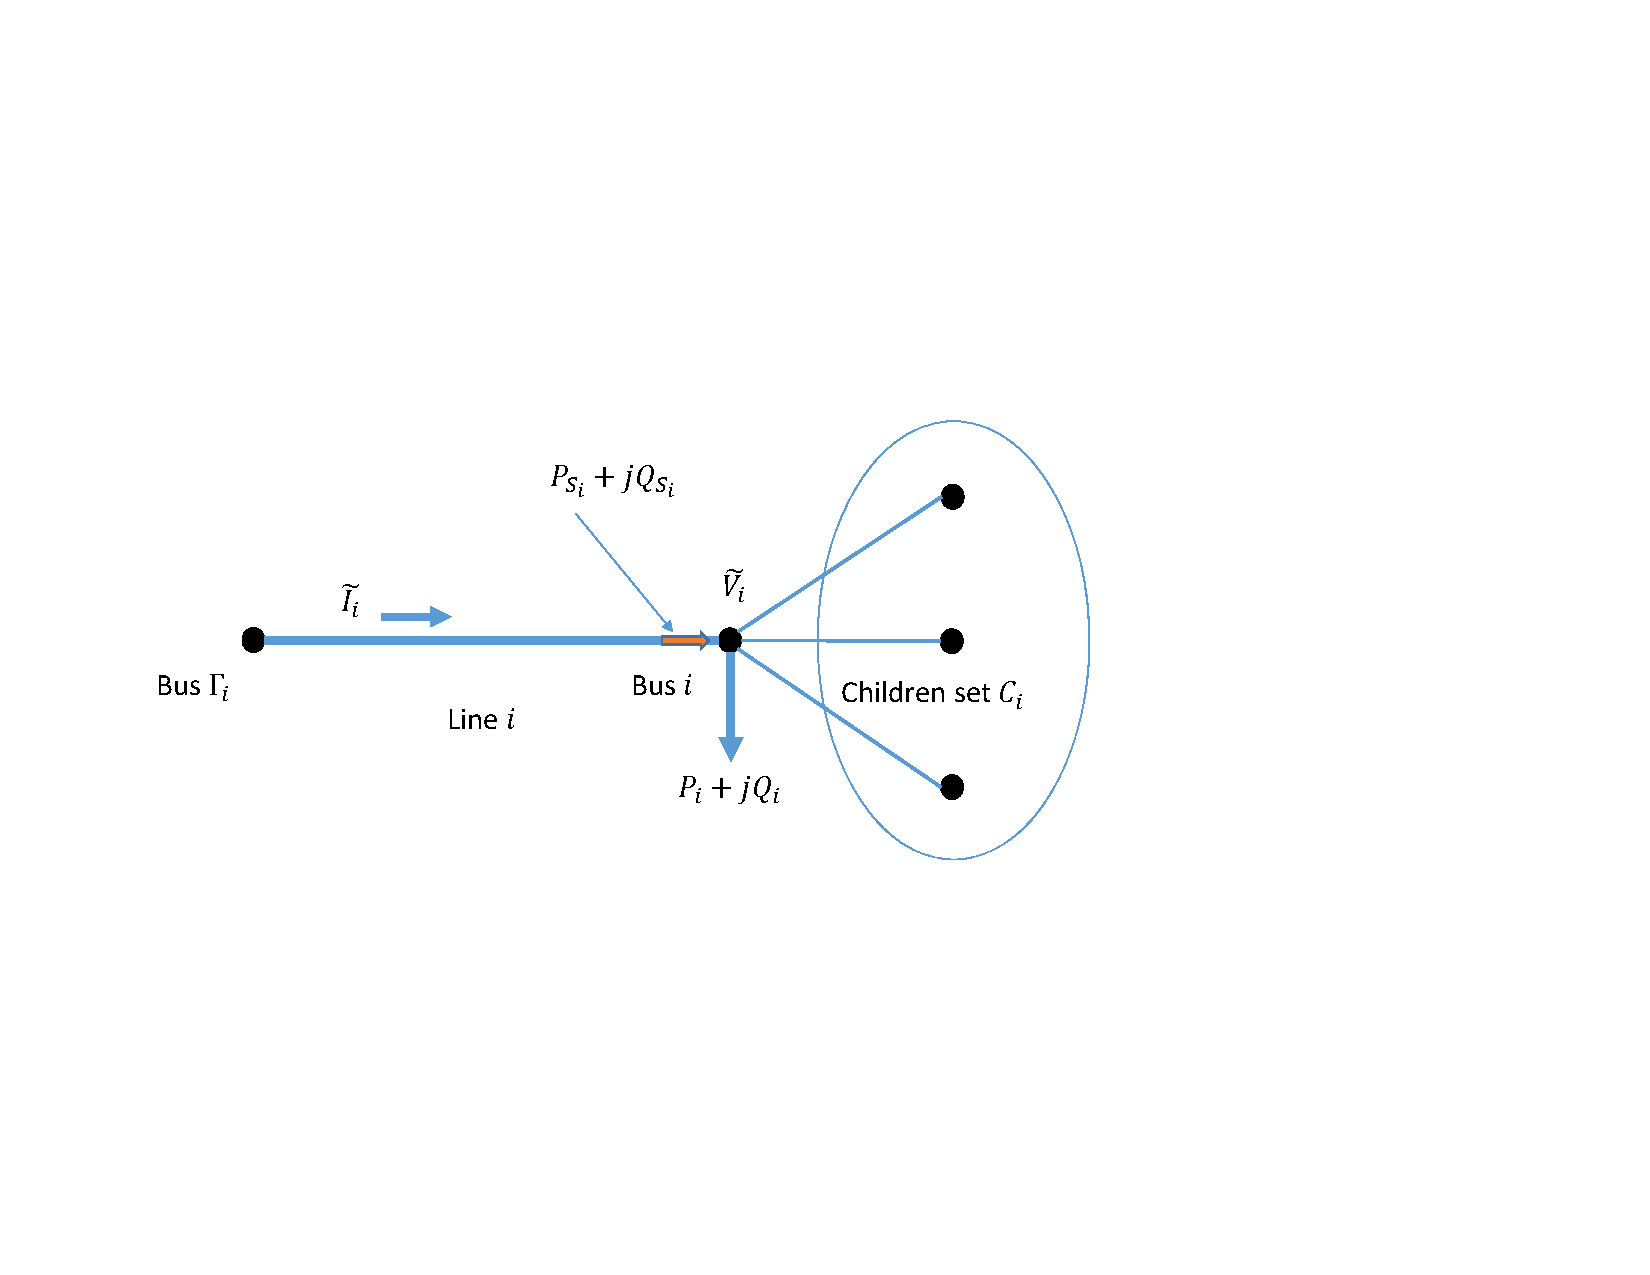
\includegraphics[width=10cm]{pics/distflow.pdf}
    \caption{Notations of distribution network}
    \label{fig:busI}
\end{figure}

To simplify the nomenclature of distribution system, the branch impedance and admittance of line $i$ are denoted by $\tilde Z_i = R_i+jX_i$ and $y_i =g_i-jb_i$ respectively, the complex current through line $i$ by $\tilde{I}_i=I_i\angle \theta_{I_i}$, and complex power at the receiving end (as shown in Figure \ref{fig:busI}) of line $i$ by $\tilde{S}_{s_i}=P_{s_i}+j Q_{s_i}$. Also, we denote the complex voltage at bus $i$ by $\tilde{ V_i }=V_i\angle \delta_{V_i}$, the angle difference by $\theta_{ik} = \theta_{i}-\theta_k\;(k\in N_i)$, and complex power injection by $\tilde{S_i} = P_i +j Q_i$. 

The bus injection power flow and branch power flow equations (Dist-Flow \cite{gan2016online}) are two commonly used models in distribution power system analysis. They are essentially equivalent on distribution systems but with different expressions: node injection power flow is a clear expression of power and voltage at all the nodes, while the branch power flow has extra information of current and power flow on each branch. The bus injection power flow equations are written as \eqref{niflow} for each node (e.g. the $i^{th}$ node):
\begin{subequations}
\label{EPower}
\begin{align}
P_{i} &= V_i^2 g_{ii} +\sum_{k \in N_i } V_{i}V_{k}(g_{k} \cos{ \theta_{ik}}+b_{k}\sin{ \theta_{ik}})\label{biflowa}\\
Q_{i} &=-V_i^2 b_{ii} +\sum_{k \in N_i} V_{i}V_{k}(g_{k}\sin{ \theta_{ik}}-b_{k} \cos{ \theta_{ik}})\label{biflowb}
\end{align}
\label{niflow}\noindent
\end{subequations}\noindent
where $g_{ii}=-\sum_{k \in C_i\cup\{i\}}g_k$, $b_{ii}=\sum_{k \in C_i\cup\{i\}}b_k$, and the conductance of bus $i$ to ground has been considered as a portion of power injection in $\tilde{S}_i$.

On the other hand, the branch power flow equations are based on each branch of the system (e.g. the $i^{th}$ line):
\begin{subequations}
\begin{align}
&\sum_{k \in C_i} (P_{s_k}+P_{L_k})= P_{s_i}  - P_i,  \label{eq:brcha}\\
&\sum_{k \in C_i} (Q_{s_k}+Q_{L_k})= Q_{s_i}   - Q_i \label{eq:brchb}, \\
&v_{\Gamma_i} - v_i = 2(R_i P_{s_i} +X_i Q_{s_i})+{|z_i|}^2\ell_i, \label{eq:brchc}\\
&{v_{i}} \ell_i = {P_{s_i}}^2 + Q_{s_i}^2,
\end{align}
\label{eq:brchflow}\noindent
\end{subequations}\noindent
where $\ell_i = I_i^2$, $v_{\Gamma_i}=V_{\Gamma_i}^2$, $v_i=V^2_{i}$, $P_{L_k}$ and $Q_{L_k}$ represents the power flow at the receiving end of the $k^{th}$ line: 
\begin{equation}
	P_{L_i}= R_i \ell_i,\;\;Q_{L_i}= X_i \ell_i,
	\label{eq:lsdf1}
\end{equation}

The physical meaning of branch model is quite straight forward: \eqref{eq:brcha} and \eqref{eq:brchb} represent the power balance of real and reactive power on the $i^{th}$ line, respectively; \eqref{eq:brchflow} is the RMS value form of power law equation. To explain \eqref{eq:brchc}, we use the following figures \ref{fig:phsor_}.
\begin{figure}[ht]
\centering
    \subfloat[Circuit]{
         %\centering
         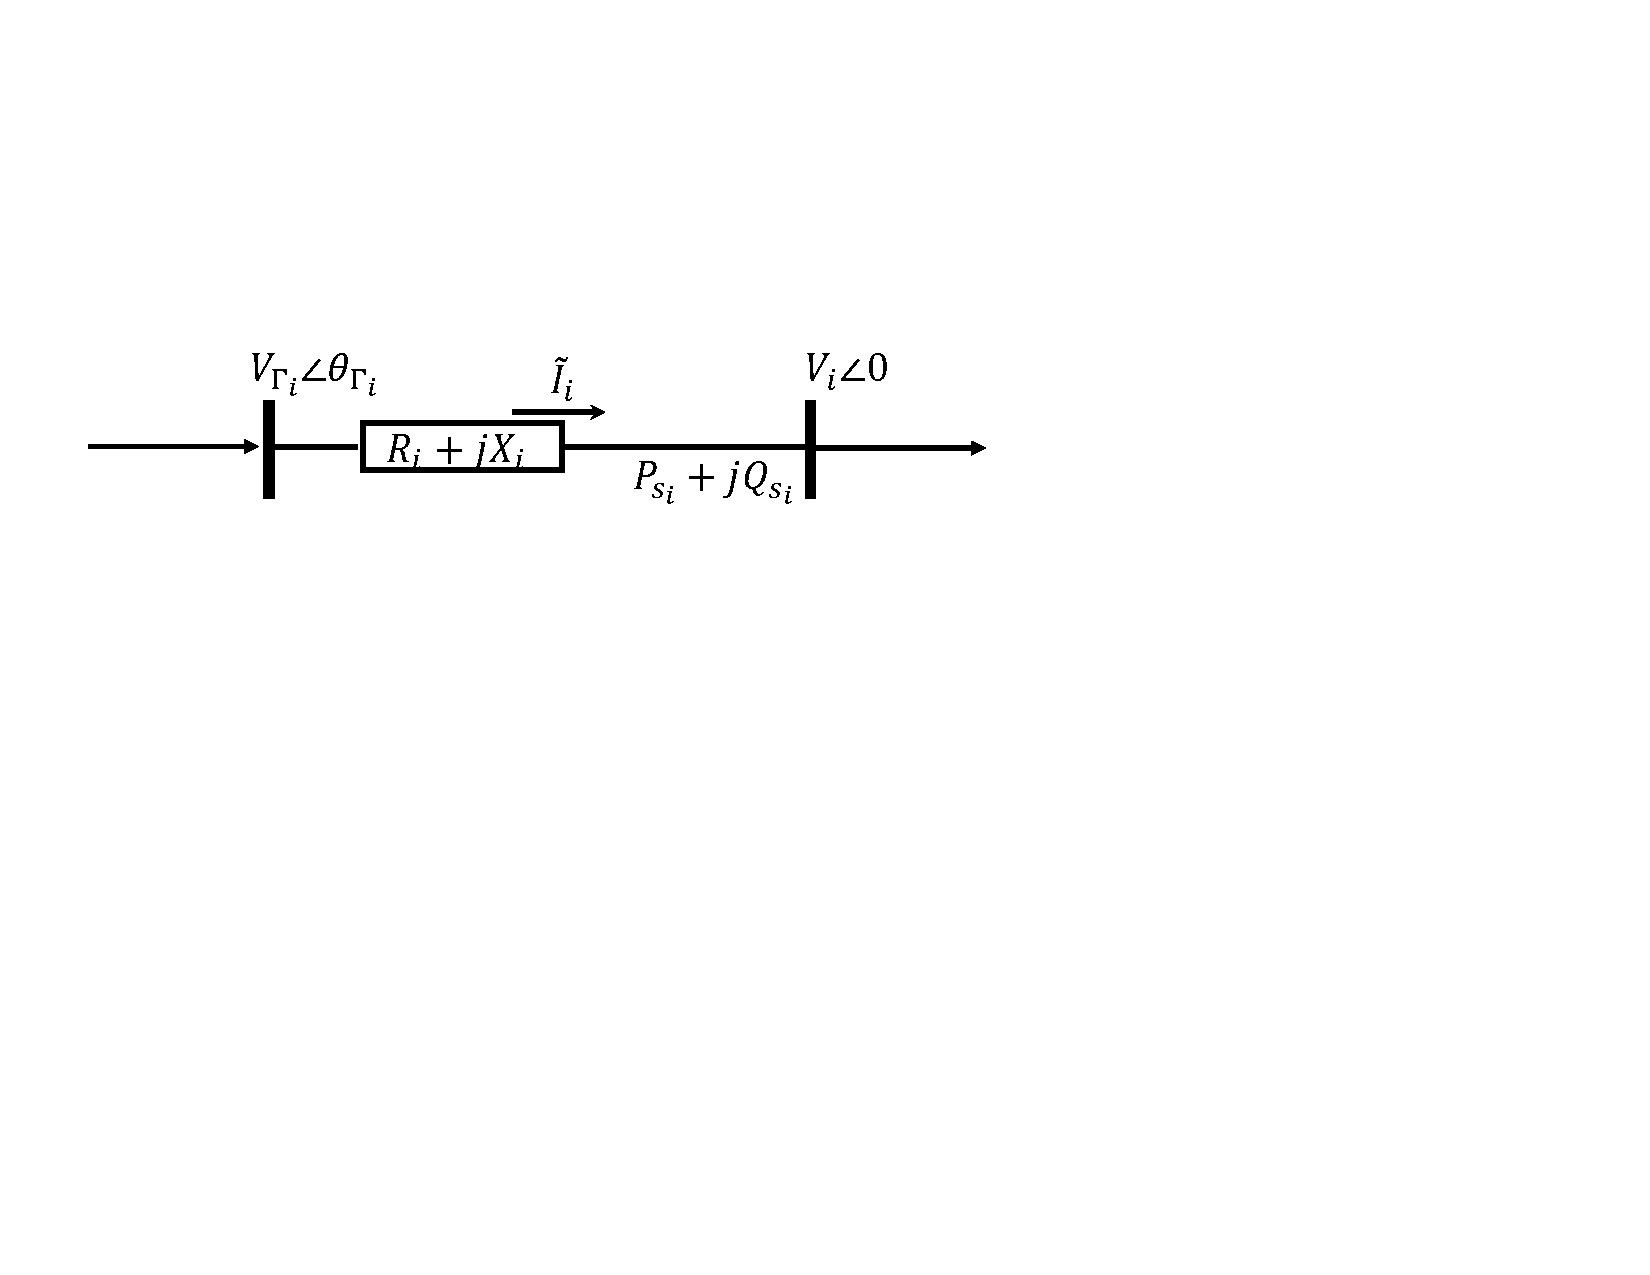
\includegraphics[width=10cm]{pics/line_i.pdf}
         %\subcaption{Circuit}
         }

    \subfloat[Phasor diagram]{
        % \centering
         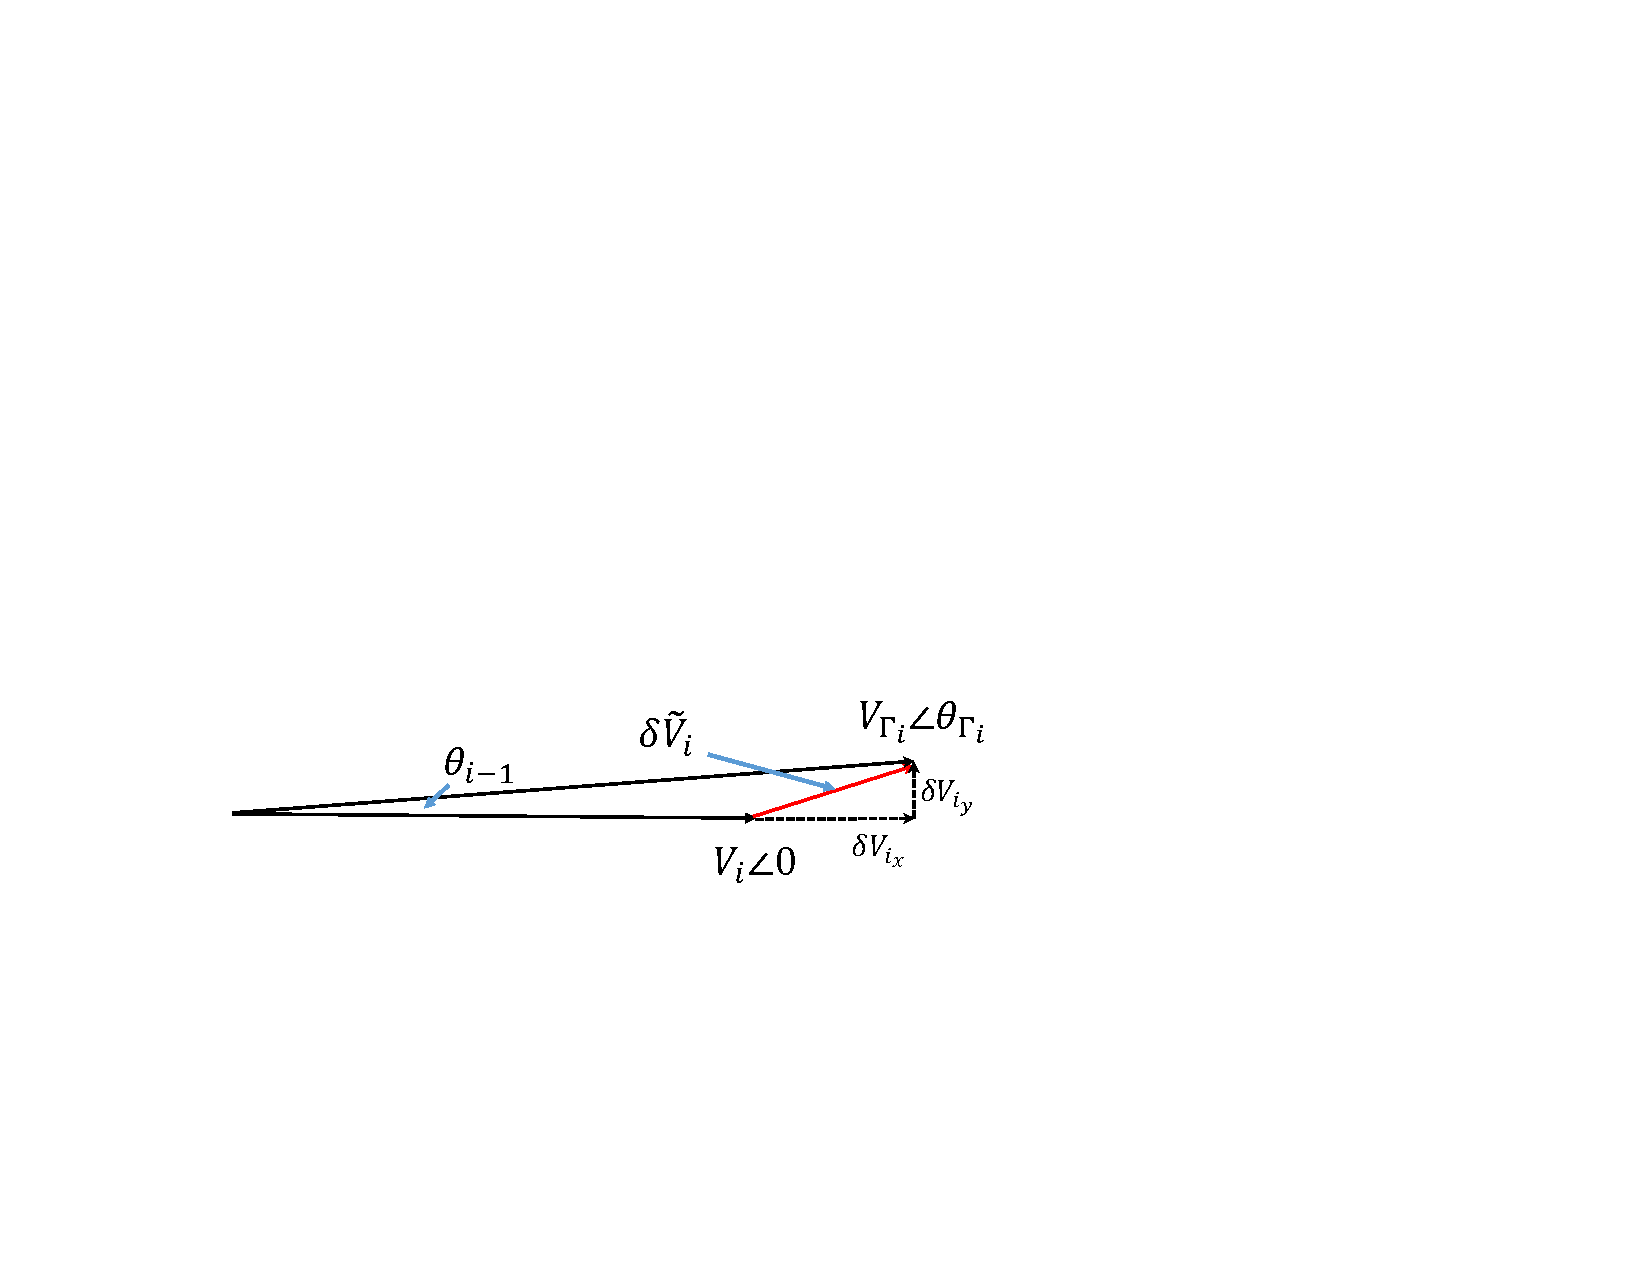
\includegraphics[width=8cm]{pics/Vector_vi.pdf}
        \label{fig:phsor_b}
         }
    \caption{The phasor notations on the $i^{th}$ line} 
    \label{fig:phsor_}
\end{figure}
In Figure \ref{fig:phsor_}, assuming the angle of $\tilde V_i$ is the reference angle and equals to zero, the angle of $\tilde V_{\Gamma_i}$ is $\theta_{\Gamma_i}$. Define the voltage difference of the $i^{th}$ bus and its parent by $\delta \tilde{V_i} = \tilde V_{\Gamma_i}-\tilde V_i $, and the real and image part of $\delta \tilde{V_i}$ are $\delta {V_{i_x}}$ and $\delta {V_{i_y}}$, respectively. It follows the Ohm's law on the $i^{th}$ line that
\begin{equation}
    \delta \tilde{V_i} = \tilde I_i (R_i+jX_i) \label{eq:dtv}
\end{equation}
and
\begin{equation}
    \tilde I_i = \frac{(P_{S_i}-jQ_{S_i})}{V_i}\label{eq:ohmi}.
\end{equation}
Substituting \eqref{eq:ohmi} into \eqref{eq:dtv} yields
\begin{equation*}
    \delta {V_{i_x}} = \frac{P_{S_i}R_i+Q_{S_i}X_i}{V_i},\;\;\delta {V_{i_y}} = \frac{P_{S_i}X_i-Q_{S_i}R_i}{V_i}.
\end{equation*}
Using triangle formula on Figure \ref{fig:phsor_b}, i.e. 
\begin{equation}
  (V_i+ \delta {V_{i_x}})^2 + \delta {V_{i_x}}^2 = V_{\Gamma_i}^2,
\end{equation}
hence \eqref{eq:brchc} can be obtained, which is actually the connection between magnitude deviation of $\tilde V_i$ from $\tilde V_{\Gamma_i}$ and the power on the $i^{th}$ line.

By substituting \eqref{eq:lsdf1} into \eqref{eq:brcha}, we have the following equation \eqref{eq:lsdf} that describes the Kirchhoff balance on $i^{th}$ line:
\begin{equation}
	P_{L_i}=  P_{s_i} + P_i-\sum_{k \in C_i}P_{s_k}.
	\label{eq:lsdf}
\end{equation}

\begin{remark}
One advantage about branch power flow \eqref{eq:brchflow} is that it offers more information on the lines, such as current, real and reactive power through the lines. Another advantage is that no angle variables are involved and hence no terms with triangular functions, which does not need angle measurements and is easier to relax the model as an convex formulation that can be solve by standard mathematical tools. 
\end{remark}
\subsection{An explicit branch model of distribution network}
The branch model of distribution network has become popular and been used in many distributed algorithm implementations in power system. For each agent, it has a nonlinear cascade form with four equations of each agent ( e.g. agent $i$ as shown in Figure. \ref{fig:busI}, including branch $i$ and bus $i$), and four variables each: the square of voltage magnitude ($v_i$), the square of current magnitude ($\ell_i$), and the power injection at bus $i$ ($P_i$ and $Q_i$). From the perspective of power system control, the injection ($P_i$ and $Q_i$) is the control and system voltage (and/or loss) is the outcome. Hence a useful transformation of \eqref{eq:brchflow}, which focuses on the effects of bus injection on system voltage, is written as following:
\begin{align}
    &v_k =-\sum_{j\in\mathcal {P}_{1k}\cup \mathcal{T}_k} [2\mathcal{R}_{kj}P_j+ 2\mathcal{X}_{kj}Q_j+(Z'_{kj} )P_{L_j}]+v_0,\label{eq:brchflowvpl}
\end{align}
where the set $\mathcal{P}_{1k}$ is defined as the path from bus $1$ to $k$; $\mathcal{T}_i$ is the node set of the subtree under node $i$; $\mathcal{R}_{kj}$, $\mathcal{X}_{kj}$, and $Z'_{kj}$ and $\gamma_j$ are network parameters (constants), i.e.
\begin{align*}
    \mathcal{R}_{kj}&=\sum_{i\in \mathcal{P}_{1j}\cap\mathcal{P}_{1k}}R_i,\;\;
    \mathcal{X}_{kj}=\sum_{i\in \mathcal{P}_{1j}\cap\mathcal{P}_{1k}}X_i,\;\;\gamma_j=X_j/R_j,\\
    Z'_{kj} &=\mathcal{R}'_{kj}+\mathcal{X}'_{kj}\gamma_j,
\end{align*} and 
\begin{equation*}
\mathcal{R}'_{kj}=
\begin{cases}
\mathcal{R}_{kj} - R_j, &\text{ if } j<=k\\
\mathcal{R}_{kj}, &\text{ otherwise}
\end{cases},\;\;
\mathcal{X}'_{kj}=
\begin{cases}
\mathcal{X}_{kj} - X_j, &\text{ if } j<=k\\
\mathcal{X}_{kj}, &\text{ otherwise}
\end{cases}.
\end{equation*}

The explicit form of power flow \eqref{eq:brchflowvpl} is derived as follows ( i.e. from \eqref{eq:vii-1} to \eqref{eq:vk}):

It follows \eqref{eq:brchflow} that
\begin{align}
v_{i-1}-v_{i}  &=2P_{S_i}R_i+2 Q_{S_i}X_i+P_{L_i}R_i+Q_{L_i}X_i,\label{eq:vii-1}
\end{align}

According to Kirchhoff law, on the subtree $\mathcal{T}_i$ , we can write the power balance equations as
\begin{align}
 P_{S_i} = P_i+\sum_{j\in \mathcal{T}_i}(P_{j}+P_{L_j}),\;\;
 Q_{S_i} = Q_i + \sum_{j\in \mathcal{T}_i}(Q_{j}+Q_{L_j}).\label{eq:psqs}
\end{align}
Plugging \eqref{eq:psqs} into \eqref{eq:vii-1}, we can then add \eqref{eq:vii-1} of all $i\in \mathcal{P}_{1k}$ together which yields
\begin{align}
v_{0}-v_{k}  =&\sum_{i\in \mathcal{P}_{1k}}\left[\right.2\sum_{j\in \mathcal{T}_i\cup\{i\}}(R_i P_j+ X_i Q_{j})\nonumber\\&+2\sum_{j\in \mathcal{T}_i}(P_{L_j} R_i+Q_{L_j}X_i)+(P_{L_i} R_i+Q_{L_i} X_i)\left.\right] \nonumber\\
=& 2\sum_{j}(P_j\sum_{i\in \mathcal{P}_{1j}\cap\mathcal{P}_{1k}}R_i+ Q_{j}\sum_{i\in \mathcal{P}_{1j}\cap\mathcal{P}_{1k}}X_i)\nonumber\\
&+2\sum_{j\in \mathcal{T}_1}(P_{L_j}\sum_{i\in\mathcal{P}_{1\min\{j-1,k\}} }R_i +Q_{L_j} \sum_{i\in\mathcal{P}_{1\min\{j-1,k\}} }X_i)\nonumber\\&+\sum_{j\in \mathcal{P}_{1k}}(R_jP_{L_j}+X_jQ_{L_j}),\label{eq:vk}
\end{align}
where $Q_{L_i}$ can be represented by $P_{L_i}$, i.e. $Q_{L_i}=\gamma_iP_{L_i}$. Hence \eqref{eq:vk} can be wrapped up as the concise form \eqref{eq:brchflowvpl}. 

\begin{note}
It is important to emphasize that the recursive model \eqref{eq:brchflowvpl} is the exact model without any approximations.  
\end{note}

From \eqref{eq:brchflowvpl}, many practical forms of distribution system equation can be easily derived by some assumptions, for example, by neglecting the system loss, \eqref{eq:brchflowvpl} becomes
\begin{equation}
    v_k =-\sum_{j\in\mathcal {P}_{1k}\cup \mathcal{T}_k} (2\mathcal{R}_{kj}P_j+ 2\mathcal{X}_{kj}Q_j)+v_0.\label{eq:vkliniear2}
\end{equation}
Given the fact that $V_k$ is always close to $1$ p.u., \eqref{eq:brchflowvpl} can be written as the following liniearized form  
\begin{equation}
    \Delta V_k =-\sum_{j\in\mathcal {P}_{1k}\cup \mathcal{T}_k} (\mathcal{R}_{kj}\Delta P_j+ \mathcal{X}_{kj}\Delta Q_j),\label{eq:vkliniear}
\end{equation}
which has been used in many distributed optimization algorithms in power system and smart grid analysis. 

\subsection{Dynamic DG model}
The above analysis does not differentiate the power generation and consumption at each bus. To illustrate the system level design, we define the generation (DGs) and consumption (loads) on each bus $i$ by $P_{g_i} + j Q_{g_i}$ and $P_{d_i} + j Q_{d_i}$ respectively, and define net injection by combining DGs generation and loads by
\begin{equation}
P_i + j Q_i =- (P_{g_i} -P_{d_i})- j (Q_{g_i}- Q_{d_i}).
\end{equation}
The detailed model of DGs will be provided as follows. 

For the simplicity of analysis, it is assumed that $P_{g_i}$ and $Q_{g_i}$ are determined by decoupled $d–q$ control method via phase locked loops (PLL), and assume inner dynamics of inverter-based DG usually diminish much faster compared to the power outputs, their control model \cite{xin2011co} can be written as
 \begin{equation}
     \left\{
     \begin{array}{cc}
          P_{g_i} &= V_i I_{p_i}   \\
          Q_{g_i} &= V_i I_{q_i} 
     \end{array}
     \right.\label{eq:dgmdl}
\end{equation} 
and
\begin{equation}
     \left\{\begin{array}{cc}
          \dot I_{p_i} &= u_{p_i}  \\
          \dot I_{q_i} &= u_{q_i}
     \end{array},\right.\label{eq:dgui}
\end{equation}
where $I_{p_i}$ and $I_{q_i}$ are the output current in $dq$-axis, $u_{p_i}$ and $u_{q_i}$ are the real/reactive power control inputs to be designed, respectively. The active and reactive power of each DG should be well controlled in their operational limits:
\begin{equation*}
    0\leq P_{g_i} \leq \overline{P}_{g_i},\;\;|Q_{g_i}| \leq \overline{Q}_{g_i},
\end{equation*}
where $\overline{P}_{g_i}$ is the maxim available real power output of each DG, and
\begin{equation}
\overline{Q}_{g_i} = \sqrt{\overline{S}_{i}^2-P_{g_i}^2},    \label{eq:qbar}
\end{equation}
$\overline{Q}_{g_i}$ is the maxim available reactive power output, and $\overline{S}_{i}$ is the apparent power capacity of the inverter, which is usually constant.

\begin{remark}
$u_{p_i}$ and $u_{q_i}$ are the real and reactive power of each DG which can be controlled to achieve specific objectives, hence providing immense potential flexibility to improve overall performance of power systems.
\end{remark}


\section{Autonomous distributed voltage control}
It is challenging for the existing centralized tools such as EMS/SCADA systems, to control thousands to millions distributed small-sized devices as described by \eqref{eq:dgmdl} in future power grids. Therefore, the distributed cooperative  control is chosen to handle this operation.
This control strategy should be built upon the distributed communication structure, with each node communicating with its neighbors. Using the cooperative control theory \cite{qu2009cooperative} and distributed subgradient based multi-agent optimization method \cite{nedic2009distributed}, the distributed voltage and frequency control in distribution network is formulated as a multi-agent problem. 

\subsection{Distributed subgradient algorithm}
We use a general form of vector $ z_i$ ($z_i \in R^n$) to represent the local information of agent $i$, and $N_i^c$ is defined as the neighboring set of the $i^{th}$ agent. Note that the ICT structure does not necessarily have the same topology connection as electrical buses in the power distribution network.\par
Utilize a binary matrix to express the communication topology as
\begin{equation}
S = \left[
\begin{array}{ccc}
s_{11}(t)&\cdots & s_{1n}(t);\\
 \vdots&  \ddots &\vdots \\
s_{n1}(t)&\cdots &s_{nn}(t)
\end{array}
\right],\label{eq:comms}
\end{equation}
where $s_{ij} = 1$ if $j \in N_i^c$ and $s_{ij} = 0$ if otherwise, for all $i,j \in \mathcal{N}$.

We start from a general multi-gent optimization problem in which agents cooperatively optimize a common additive objective function. Each agent minimizes its own cost function, and communicates with other agents,
\begin{equation}
\min \sum_{i\in \mathcal{N}} f_i(z)
\label{opt}
\end{equation}
where $f_i$ is the distributed cost function of agent $i$ with a convex form. Denote the optimal value of \eqref{opt} by $f^*$, and the optimal solution set by $Z^*$, which is $Z^* = \{ z \in | \sum_{i\in \mathcal{N}} f_i(z) = f^*\}$ .\par
In this setting, the information state $z_i$ is an estimate of the optimal solution of \eqref{opt}. Each agent updates its estimate first, then exchanges information with others; then updates itself again, and iterates until converging. We propose the close-loop cooperative control law based on the conclusion of \cite{nedic2009distributed}:
\begin{equation}
z_i(k+1) = \sum_{j \in N_i^c}d_{ij} z_j(k) - \beta_i g_{i}(k).
\label{eq:ccl}
\end{equation} 
where $k$ denotes the iteration; the vector $g_{i}$ is a subgradient of control objective function $f_i$ of agent $i$ with respect to $z_i$; $\beta_i$ is the step size used by the $i^{th}$ agent; $d_{ij}$ denotes the weights of communication topology:
\begin{equation}
 d_{ij} =\frac{w_{ij} s_{ij}}{\sum_{j\in N_i^c}w_{ij} s_{ij}},    \label{eq:dij}
\end{equation}
$w_{ij}>0$ are the weights and all $w_{ij}=1$ for symmetric systems which is true for all power systems. 

\subsection{Distributed subgradient voltage control}
In this section, the distributed control algorithm is implemented through DG inverters to cooperatively control real and reactive power generation of each DG, so that the system voltage performance can be well maintained in order to satisfy the regulation requirement, as follows:
\begin{equation}
    |1-V_i |\leq 0.05.
\end{equation}
Therefore the distributed objective function is design to minimize the voltage deviation at the $i^{th}$ bus, which is:
\begin{equation}
    f_i =\frac{\lambda^v_i}{2}(V_i-V_i^{ref})^2+\frac{\lambda^p_i}{2}(P_{g_i}-P^{ref}_{g_i})^2+\frac{\lambda^q_i}{2}Q_{g_i}^2,\label{eq:fiv}
\end{equation}
where the last two terms are designed to minimize the real power curtailment and the reactive power utlization; $V_i^{ref}$ and $P_i^{ref}$ are the reference voltage and power respectively at the $i^{th}$ bus and can be obtained from OPF or other regulatory level design, e.g. $V_i^{ref}=1$ and $P_{g_i}^{ref}=\overline{P}_{g_i}$; $\lambda^v_i\geq 0$, $\lambda^p_i\geq 0$ and $\lambda^q_i\geq 0$ are the weighting coefficients. 

We first justify that \eqref{eq:fiv} is convex by the following steps: $\frac{\lambda^v_i}{2}(V_i^{ref}-V_i)^2$ is proved in \cite{azwirman2019res,Gusrialdi2019} to be strictly convex with respect to $Q_{g_i}$ in the context of power system operation; by the the same procedure, it is straightforward to prove that it is also strictly convex with respect to $P_{g_i}$; the last two terms $\frac{\lambda^p_i}{2}(P_{g_i}-P^{ref}_{g_i})^2$ and $\frac{\lambda^q_i}{2}Q_{g_i}^2$ are also convex. 

One way to implement the distributed subgradient control \eqref{eq:ccl} for voltage control is the fair utilization ratio method \cite{maknouninejad2014realizing}, which uses the utilization ratios of real and reactive power at the $i^{th}$ bus as the control variables, i.e.
 \begin{subequations}
\begin{align}
    \alpha_{p_i} &\overset{\Delta}{=} \frac{P_{g_i}}{\overline P_{g_i}},\label{eq:alfap}
\\
    \alpha_{q_i} &\overset{\Delta}{=} \frac{Q_{g_i}}{\overline Q_{g_i}}.\label{eq:alfaq}
\end{align}
\label{eq:alfa}\noindent
\end{subequations}

Hence the subgradient of each agent, which is defined by $g_i$ in \eqref{eq:ccl}, can be calculated by taking the derivative of $ f_i$ with respect to $\alpha_{p_i}$ and $\alpha_{q_i}$ as follows:
\begin{subequations}
 \begin{align}
g^p_i&=\frac{\partial f_i}{\partial\alpha_{p_i}}=(\lambda^v_i\frac{\partial f_i}{\partial V_i}\frac{\partial V_i}{\partial P_{g_i}}+\lambda^p_i(P_{g_i}-P^{ref}_{g_i}))\frac{\partial P_{g_i}}{\partial\alpha_{p_i}},     \label{eq:gip}
\\
 g^q_i&=\frac{\partial f_i}{\partial\alpha_{q_i}}=(\lambda^v_i\frac{\partial f_i}{\partial V_i}\frac{\partial V_i}{\partial Q_{g_i}}+\lambda^q_iQ_{g_i})\frac{\partial Q_{g_i}}{\partial\alpha_{q_i}}. \label{eq:giq} 
 \end{align}
 \label{eq:gi}
\end{subequations}
It follows \eqref{eq:fiv} and \eqref{eq:alfa} that 
\begin{equation}
\frac{\partial f_i}{\partial V_i}=V_i-V_i^{ref}.\label{eq:gi1}
\end{equation}
and 
\begin{subequations}
\begin{align}
\frac{\partial P_{g_i}}{\partial \alpha_{p_i}}&={\overline  P_{g_i}}, 
\\
\frac{\partial Q_{i}}{\partial \alpha_{q_i}}&={\overline Q_{g_i}}.\label{eq:gi2}
\end{align}\label{eq:dalfapq}\noindent
\end{subequations}
By taking the derivative of power flow \eqref{niflow}, one can get the following equations for real/reactive power versus bus voltage:
\begin{equation}
\begin{split}
\frac{\partial Q_i}{\partial V_i} &=-2 V_i b_{ii}+\sum_{k \in N_i} V_{k}(g_{k}\sin{ \theta_{ik}}-b_{k} \cos{\theta_{ik}})\\
    =&\frac{Q_i-V_i^2 b_{ii}}{V_i},
\end{split}\label{eq:qv}
\end{equation}
and
\begin{equation}
\begin{split}
\frac{\partial P_i}{\partial V_i} &=2 V_i g_{ii}+\sum_{k \in N_i} V_{k}(g_{k}\cos{ \theta_{ik}}+b_{k} \sin{\theta_{ik}})\\
    =&\frac{P_i+V_i^2 g_{ii}}{V_i}.
\end{split}\label{eq:pv}
\end{equation}
Without loss of generosity, lets assume $\frac{\partial P_{i}}{\partial V_i}=\frac{\partial P_{g_i}}{\partial V_i}$ and $\frac{\partial Q_{i}}{\partial V_i}=\frac{\partial Q_{g_i}}{\partial V_i}$. Then following \eqref{eq:qv} and \eqref{eq:pv}, the derivatives of bus voltage with respect to real/reactive power generation of DG can be written as
\begin{subequations}
\begin{align}
\frac{\partial V_i}{\partial P_{g_i}} &= \frac{V_i}{P_i+V_i^2 g_{ii}},
    \label{eq:givp}\\
    \frac{\partial V_i}{\partial Q_{g_i}}  &= \frac{V_i}{Q_i-V_i^2 b_{ii}}.
    \label{eq:givq}
\end{align}\label{eq:givpq}
\end{subequations}
Plugging \eqref{eq:gi1}, \eqref{eq:dalfapq} and \eqref{eq:givpq} into \eqref{eq:gi} yields the subgradient formula: 
\begin{subequations}
\begin{align}
  g^p_i&=\overline P_{g_i}\left[\lambda^v_i(V_i-V_i^{ref}) \frac{V_i}{P_i+V_i^2 g_{ii}}+\lambda^p_i(P_{g_i}-P^{ref}_{g_i})\right]
\\
g^q_i&=\overline Q_{g_i}\left[\lambda^v_i(V_i-V_i^{ref}) \frac{V_i}{Q_i-V_i^2 b_{ii}}+\lambda^q_iQ_{g_i}\right]
\end{align}\label{eq:gipq}\noindent
\end{subequations}
It can be inferred from \eqref{eq:gipq} that the subgradient calculation of voltage control for each agent only requires local information. In summary, the continuous form of distributed real power control is written as
\begin{equation}
    \dot \alpha_{p_i} = \sum_{j \in N_i^c}d_{ij} (\alpha_{p_j}-\alpha_{p_i}) - \beta_i g^p_{i},  \label{eq:dalfap}
\end{equation}
and the reactive power control is \begin{equation}
    \dot \alpha_{q_i} = \sum_{j \in N_i^c}d_{ij} (\alpha_{q_j}-\alpha_{q_i}) - \beta_i g^q_{i}. \label{eq:dalfaq}
\end{equation}

\begin{figure}[ht]
    \centering
    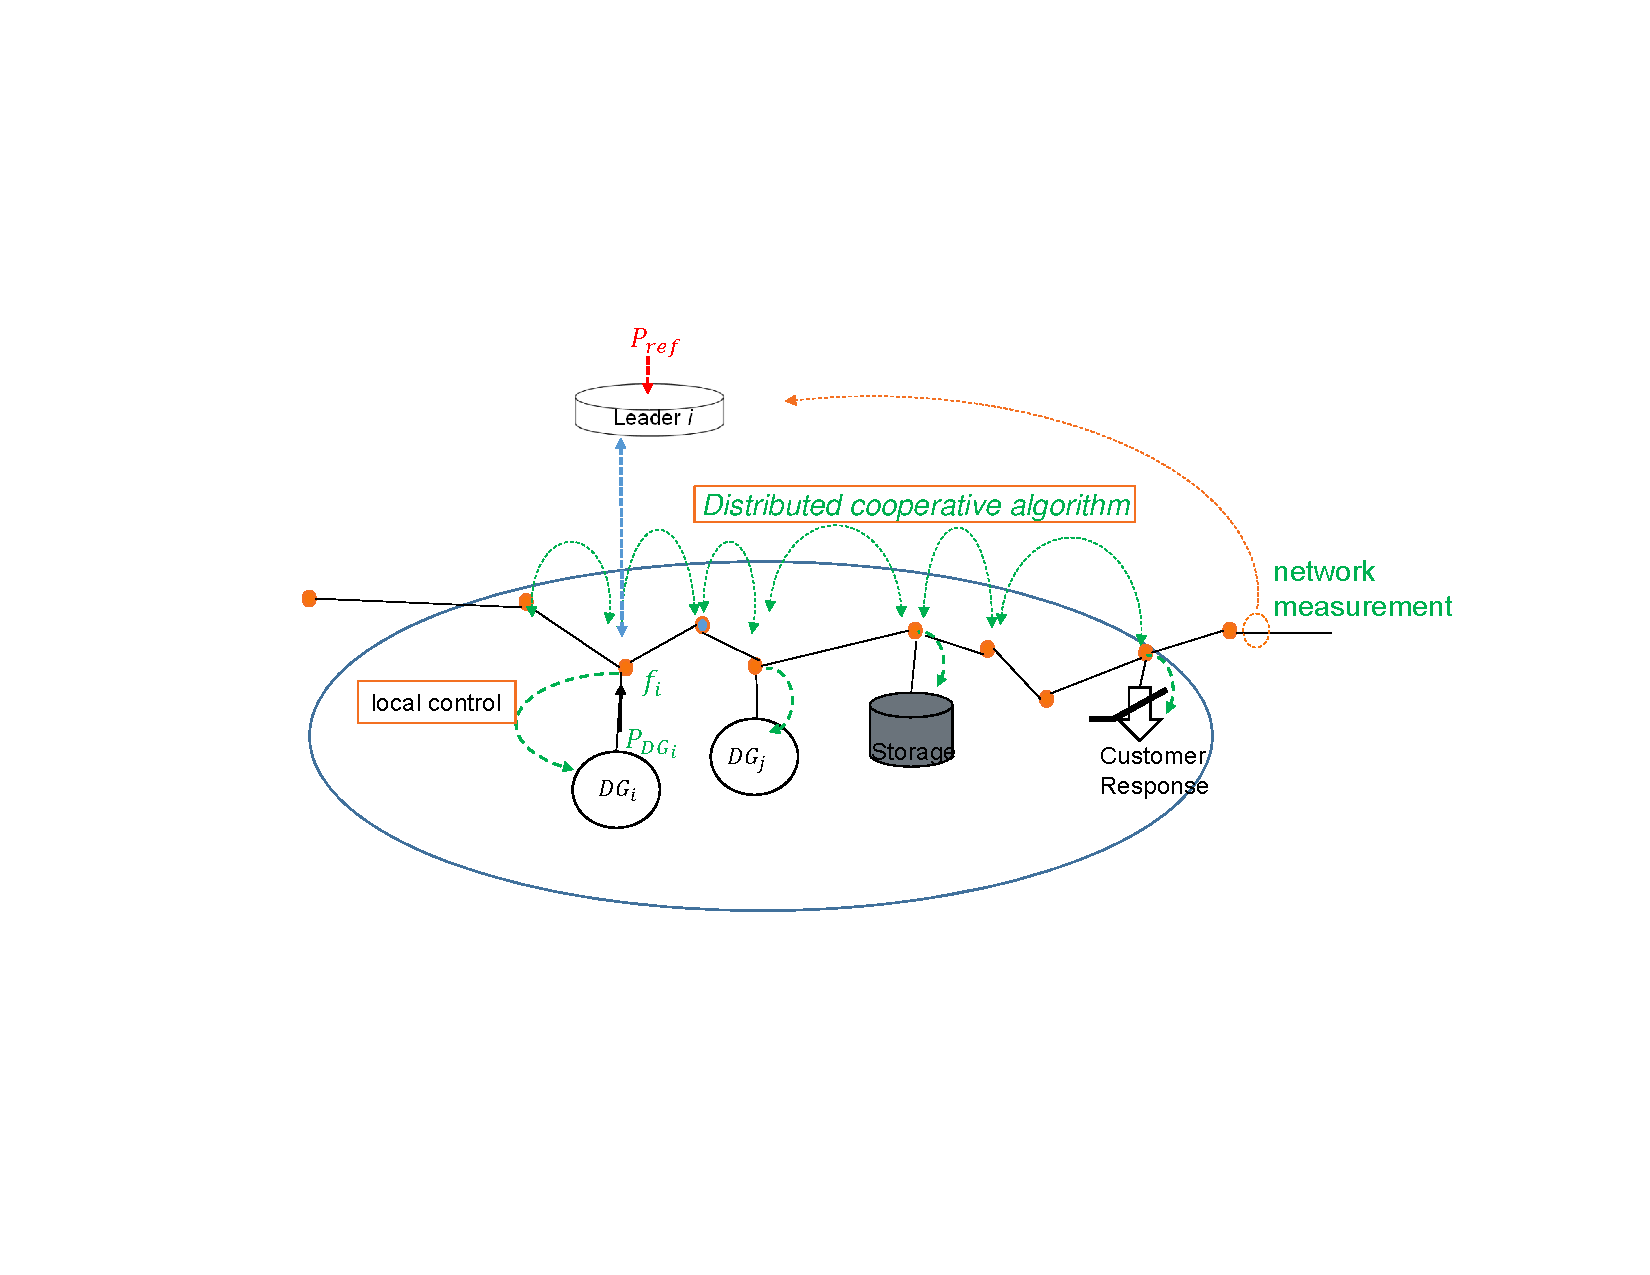
\includegraphics[width=\linewidth]{pics/pf_ctrl.pdf}
    \caption{Distributed voltage control}
    \label{fig:pfctrl}
\end{figure}

The overview of the distributed cooperative voltage control is shown by Figure \ref{fig:pfctrl}. To synthesize the above control into the feedback loop of each DG as defined by \eqref{eq:dgmdl}, we take derivative of \eqref{eq:dgmdl} and \eqref{eq:alfa}, then we get the following equations:
\begin{subequations}
\begin{align}
    \dot P_{g_i} &= V_i \dot I_{p_i} = V_i u_{p_i} \label{eq:dpu}\\
    \dot Q_{g_i} &= V_i \dot I_{q_i} = V_i u_{q_i} \label{eq:dqu}
\end{align}
\end{subequations}
and
\begin{subequations}
\begin{align}
    \dot P_{g_i} &= \overline{P}_{g_i} \dot \alpha_{p_i},\label{eq:dpalfap}\\
    \dot Q_{g_i} &= \overline{Q}_{g_i} \dot \alpha_{q_i} + \dot {\overline Q}_{g_i} \alpha_{q_i},\label{eq:dqalfaq}
\end{align}
\end{subequations}
where $V_i$ and $\overline{P}_{g_i}$ should be measured from the bus, and $\dot {\overline Q}_{g_i}$ can be obtained from \eqref{eq:qbar}, i.e.
\begin{equation}
    \dot {\overline Q}_{g_i} =- \frac{\overline{P}_{g_i}}{ {\overline Q}_{g_i}}\dot \alpha_{p_i}.\label{eq:dqbar}
\end{equation}
Thus by \eqref{eq:dqu}, \eqref{eq:dqalfaq} and \eqref{eq:dqbar}, the reactive power control of the $i^{th}$ DG, $u_{q_i}$, is written as
\begin{equation}
\begin{split}
    u_{q_i} =&\frac{\overline{Q}_i}{V_i} \dot \alpha_{q_i}- \frac{ \alpha_{q_i} \overline{P}_{g_i}} {\overline Q_{g_i}V_i}\dot \alpha_{p_i}
    \\=& \frac{\overline{Q}_i}{V_i} \left [\sum_{j \in N_i^c}d_{ij} (\alpha_{q_j}-\alpha_{q_i})- \beta^q_i g^q_{i}\right] \\&-\frac{ \alpha_{q_i} \overline{P}_{g_i}}{\overline Q_{g_i}V_i} \left [\sum_{j \in N_i^c}d_{ij} (\alpha_{p_j}-\alpha_{p_i}) - \beta^p_i g^p_{i}\right] .
\end{split}\label{eq:uqirslt}
\end{equation}
Similarly, using \eqref{eq:dpu} and \eqref{eq:dpalfap}, the real power control $u_{p_i}$ is written as
\begin{equation}
    u_{p_i} = \frac{\overline{P}_i}{V_i} \dot \alpha_{p_i} = \frac{\overline{P}_i}{V_i} \left [\sum_{j \in N_i^c}d_{ij} (\alpha_{p_j}-\alpha_{p_i}) - \beta^p_i g^p_{i}\right].\label{eq:upirslt}
\end{equation}
\begin{note}
According to \eqref{eq:uqirslt}, $u_{q_i}$ is dependant on $\alpha_{p_i}$. The reason is the control strategy of real power control priority is adopted. $u_{p_i}$ and $u_{q_i}$ can have other forms according to different control priorities, but the derivation should be the same.
\end{note}

The performance of the proposed voltage control has been evaluated on multiple test systems such as: IEEE 123-bus, 8500-node, and other standard systems \cite{rathbun2018impact}. To show the effectiveness of the proposed approach on even larger scale systems, a 100,000 (100k)-node circuit is built by combining different type of feeders: the circuit is assembled by 12 urban/suburban feeders, as shown in Figure \ref{fig:C1ckts}. 
\begin{figure}[ht]
\centering

         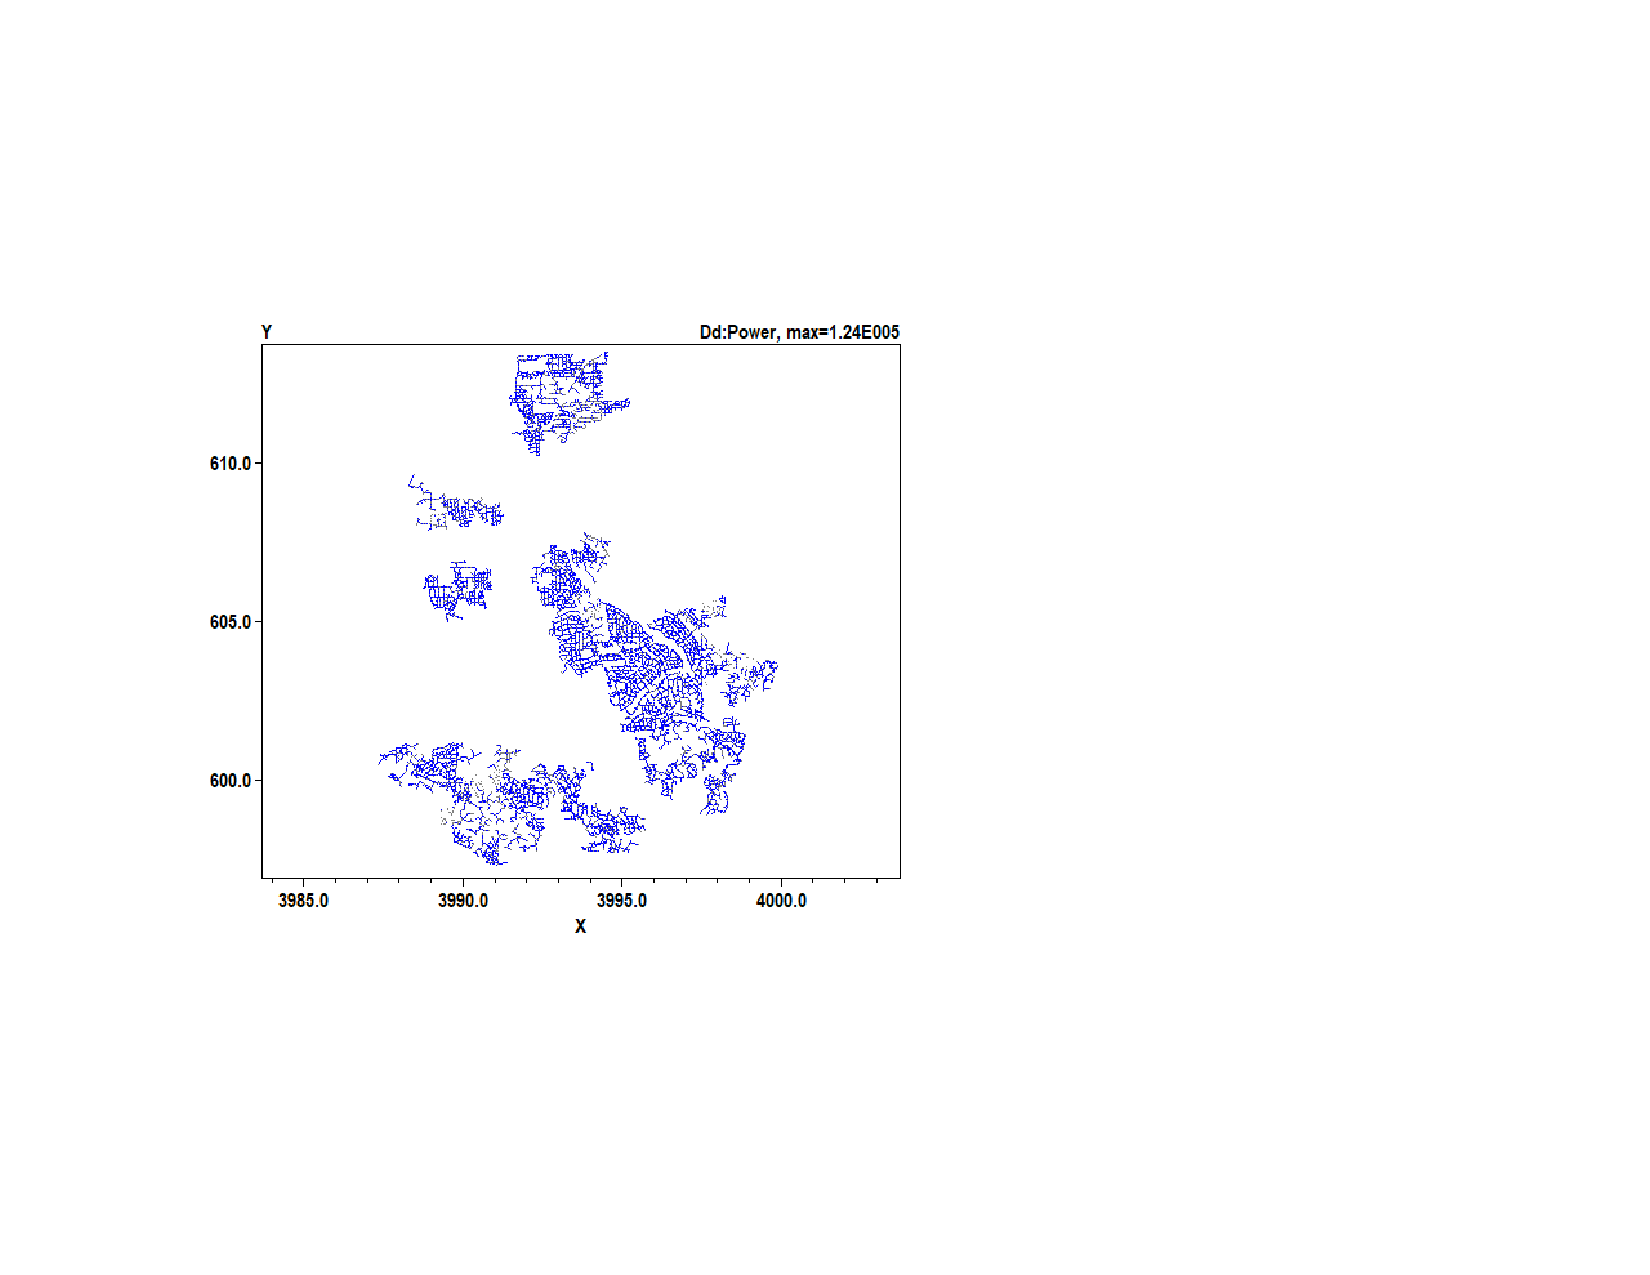
\includegraphics[width=8cm]{pics/C1.pdf}
         %\subcaption{Circuit}

    \caption{100k synthetic circuits}
    \label{fig:C1ckts}
\end{figure}

\begin{figure}
\centering
\subfloat[Scenario 1]{
         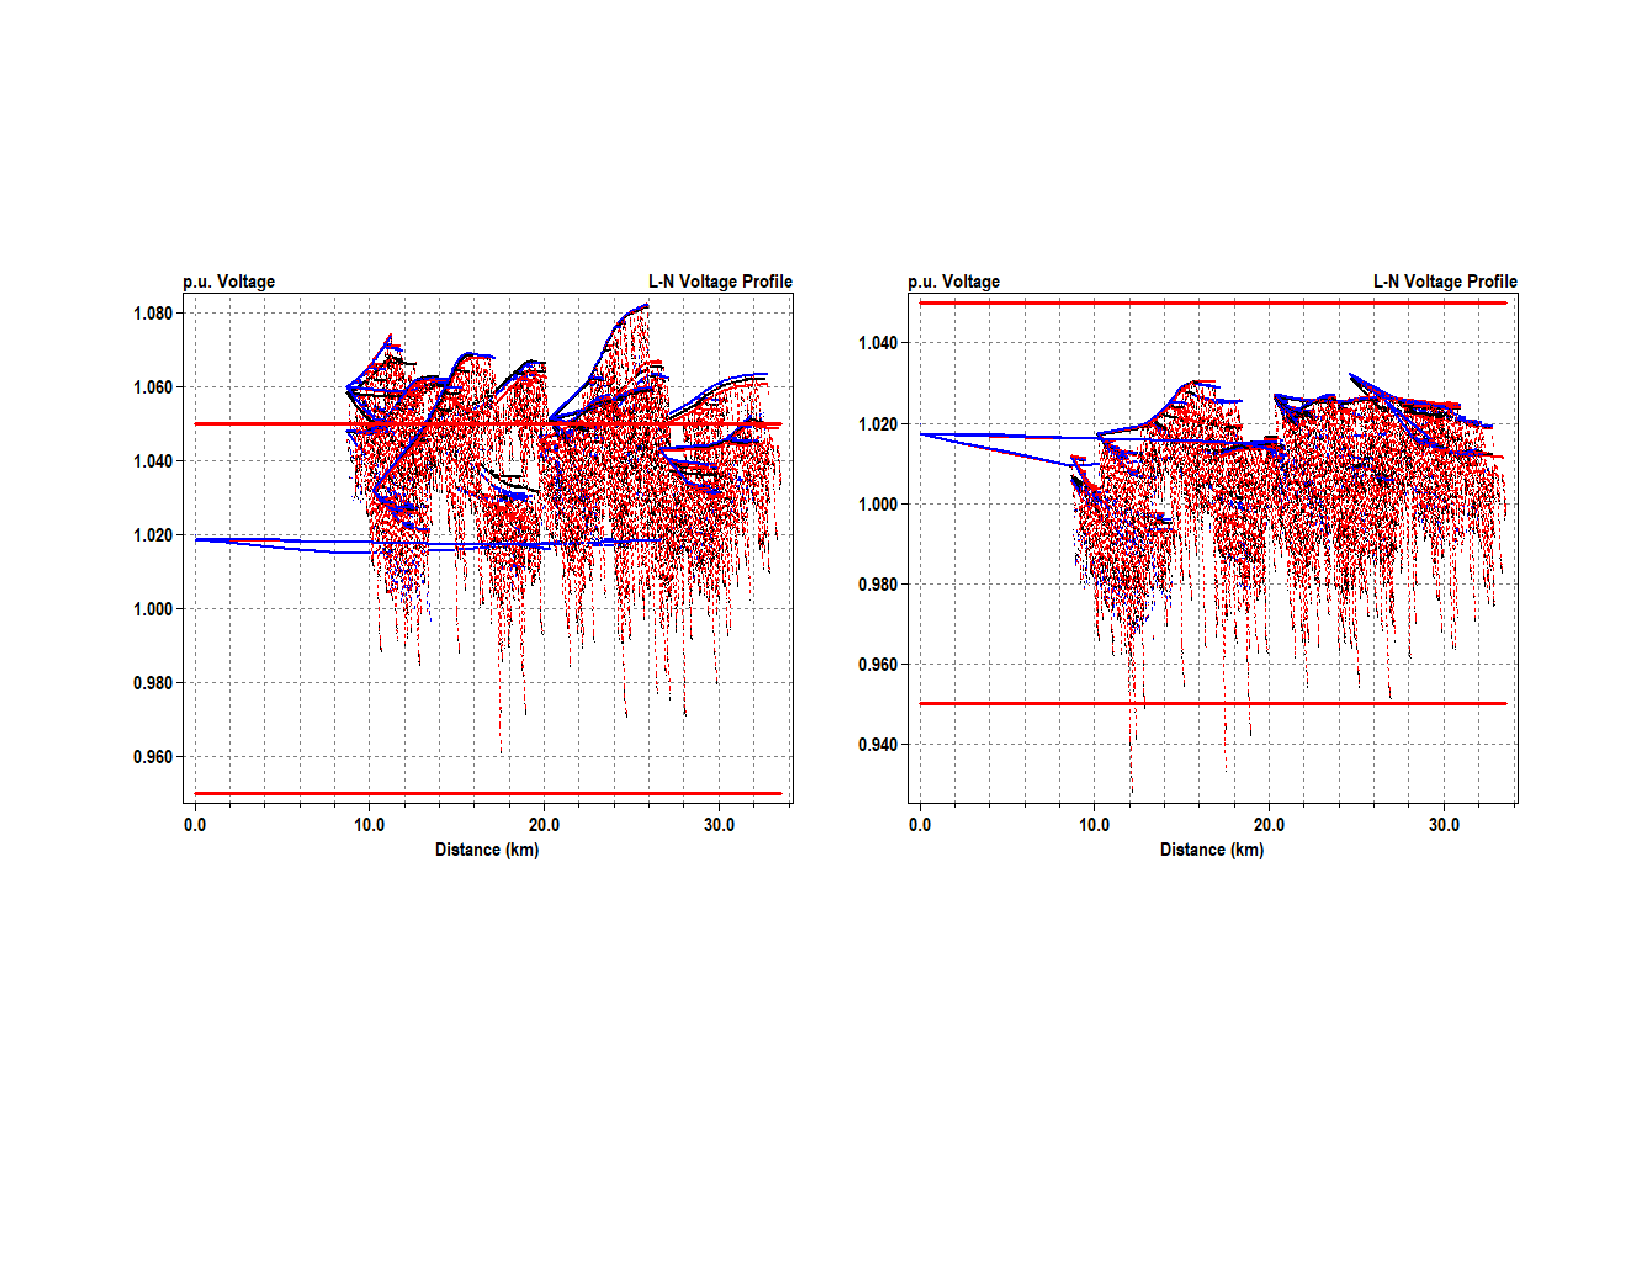
\includegraphics[width=\linewidth]{pics/C1_lg.pdf}
}
\quad
\subfloat[Scenario 2]{
         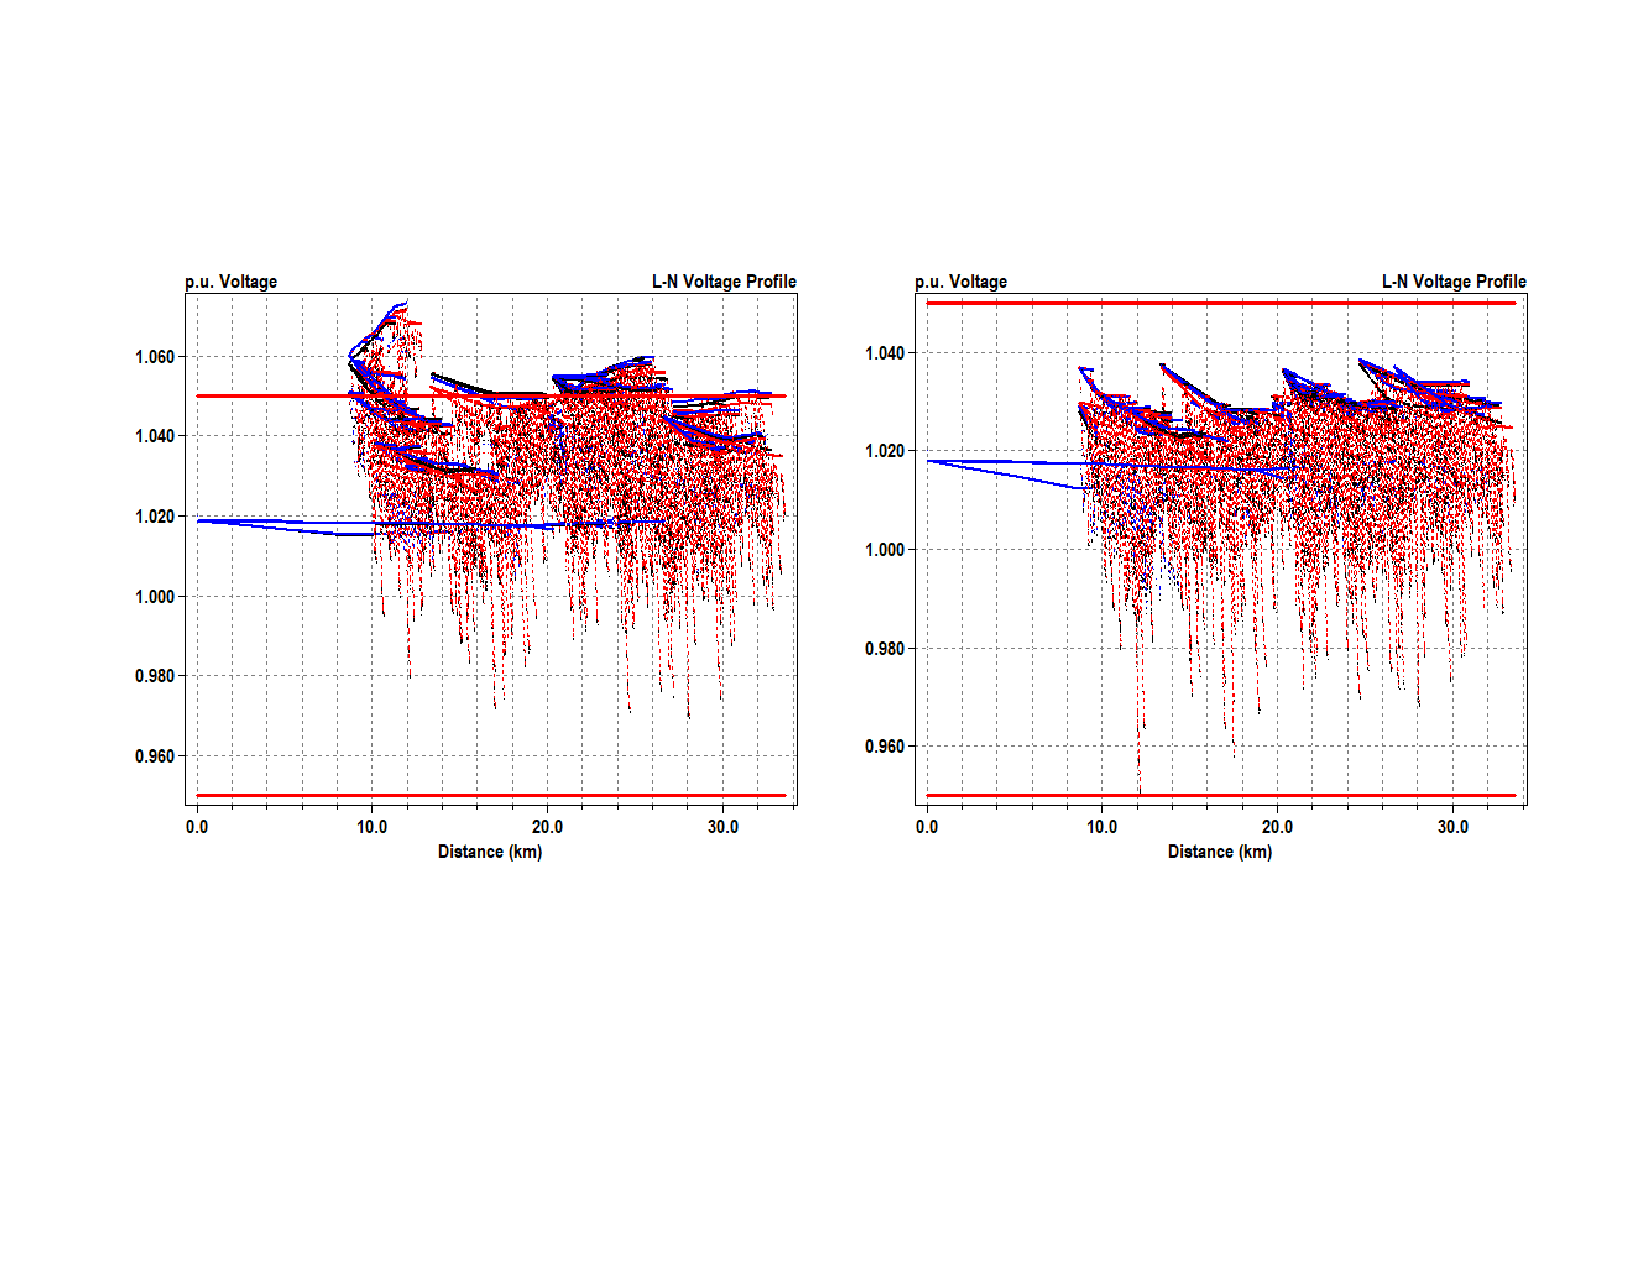
\includegraphics[width=\linewidth]{pics/C1_dis.pdf}
}
\quad
\subfloat[Scenario 1: Details]{
         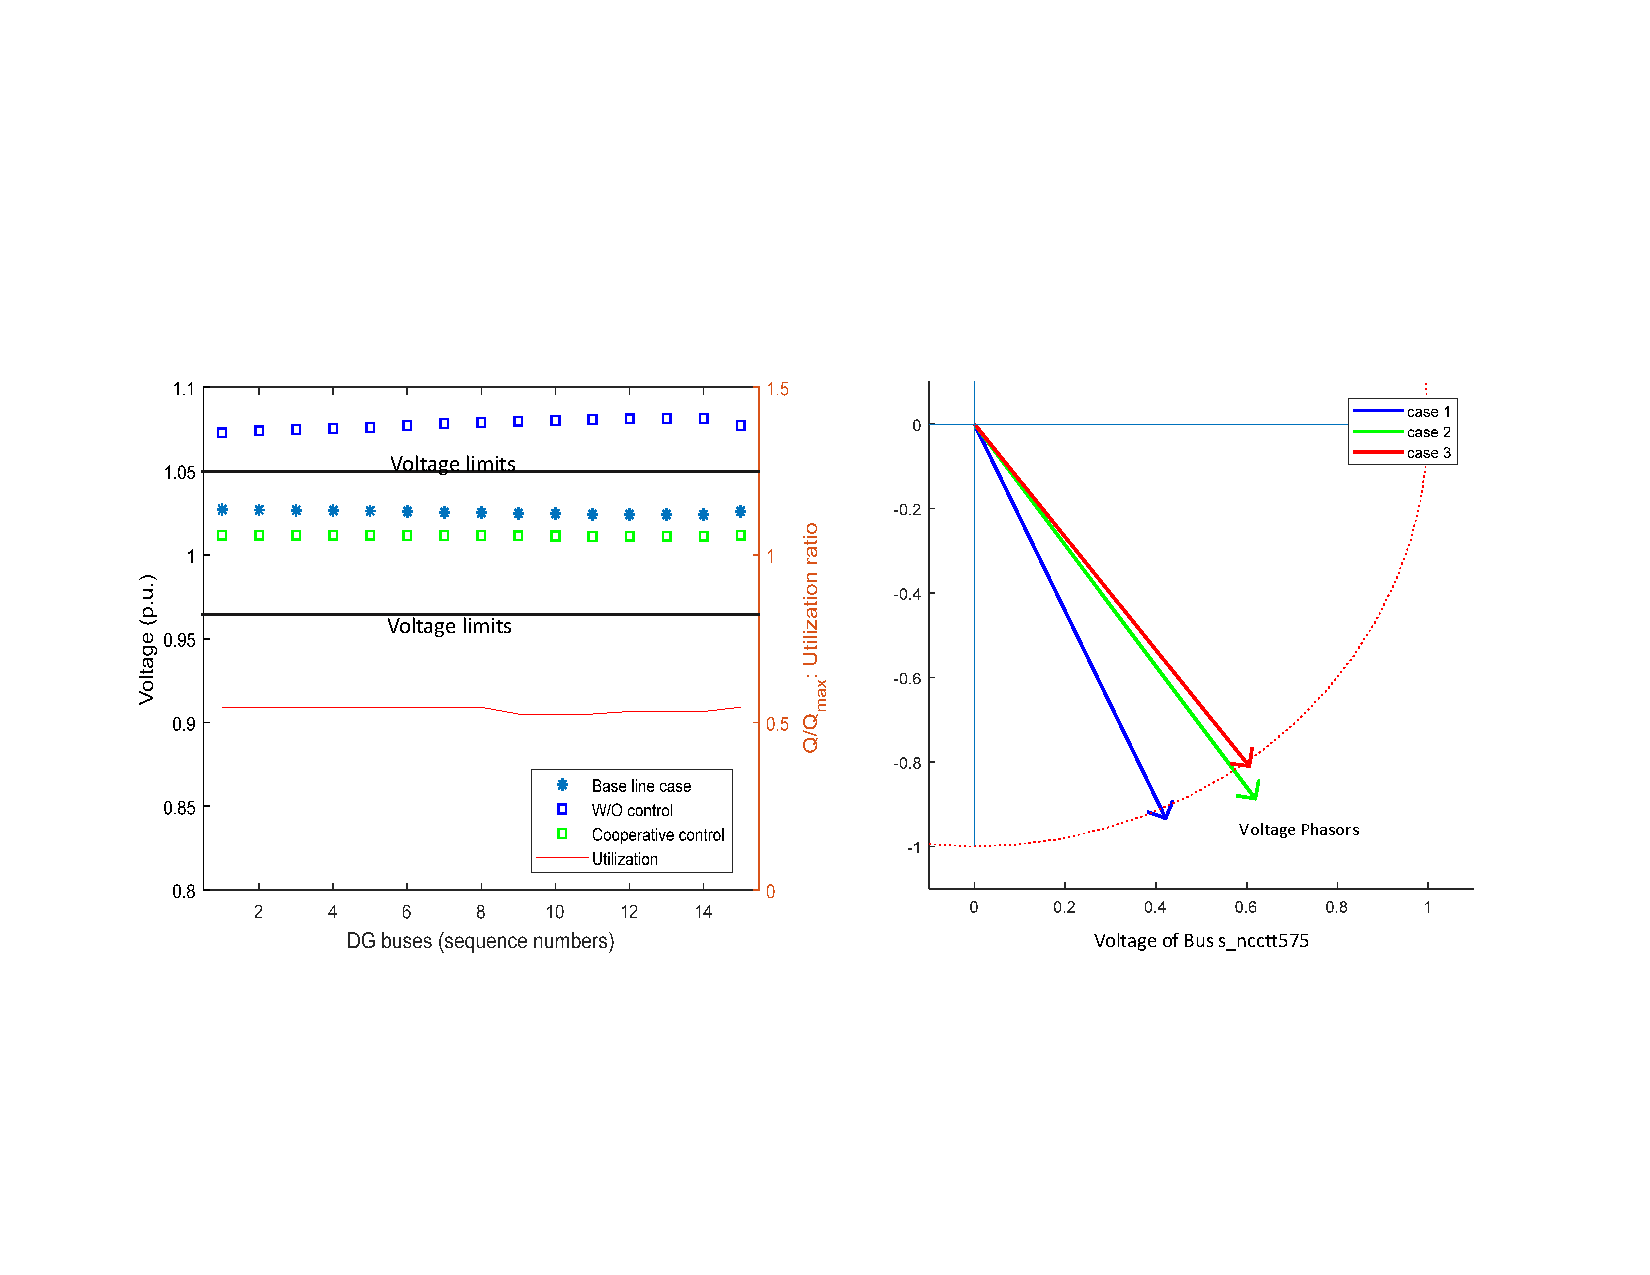
\includegraphics[width=\linewidth]{pics/volctrl_dtls.pdf}
        \label{fig:rslt_s1_dtls}
}
    \caption{Results of voltage control on 100k synthetic circuits}
    \label{fig:C1_ckts_rslt}
\end{figure}
The total load of the circuit is 122MW. On top of the physical layer, 268 clusters are predefined for communication and control. Assume all load tap changers (LTCs) in the circuit are fixed at the predefined positions during the fast control of inverters. Two extremely harsh scenarios developed by the greedy search method \cite{rathbun2018impact} are studied: Case 1 defines 104 large scale PVs among 12 feeders, which is the large scale PV Farms scenario; Case 2 defines 2528 PVs distributed across the network, which is the distributed PVs scenario. In both cases, each of the feeders is self-balanced in terms of its own PV generation and load consumption, and the load in each feeder is evenly distributed among PVs.

Simulation results of both cases show that the proposed cooperative reactive power control can effectively regulate the system voltages for distributed PVs, as shown in Figure \ref{fig:C1_ckts_rslt}. The spatial voltage profile of all phases is shown in Figure \ref{fig:C1_ckts_rslt}, where Y-axis is the p.u. value of bus voltages and X-axis denotes the distance from substation. In Scenario 1, a total 37MVar of inductive reactive power is generated by PV inverters to suppress the voltage violation; the highest inverter capacity is 108.6$\%$. In Scenario 2, a total 22MVar of inductive reactive power is generated by PV inverters; the highest inverter capacity is 103.3$\%$. Note that it is easier for the distributed scenario is to control the voltage.

To better illustrate the control effect, the detailed information about about one part of the 100k system in Scenario 1 is shown in Figure \ref{fig:rslt_s1_dtls}. As shown by the results, the voltage is controlled within in the limits, and reactive power utilization ratios of all DGs in each feeder reach consensus.

\subsection{Reactive power control and power factor control}
The voltage control scheme aims to hold the system voltage by the inverter's ability of offering reactive power support at DG buses.
Following \eqref{eq:vkliniear}, to control system voltage autonomously, the reactive power of DGs must respond to the real power injection of renewables. As a result, the reactive power at the feeder (the slack bus) would change accordingly, hence the power factor at the substation will fluctuate and sometimes it might not be acceptable to the transmission side. To illustrate the effect of autonomous control on power factor, a simplified system with two concentrated loads and one aggregated DG is used, as shown in Figure \ref{fig:3bussys}.


\begin{figure}[ht]
    \centering
    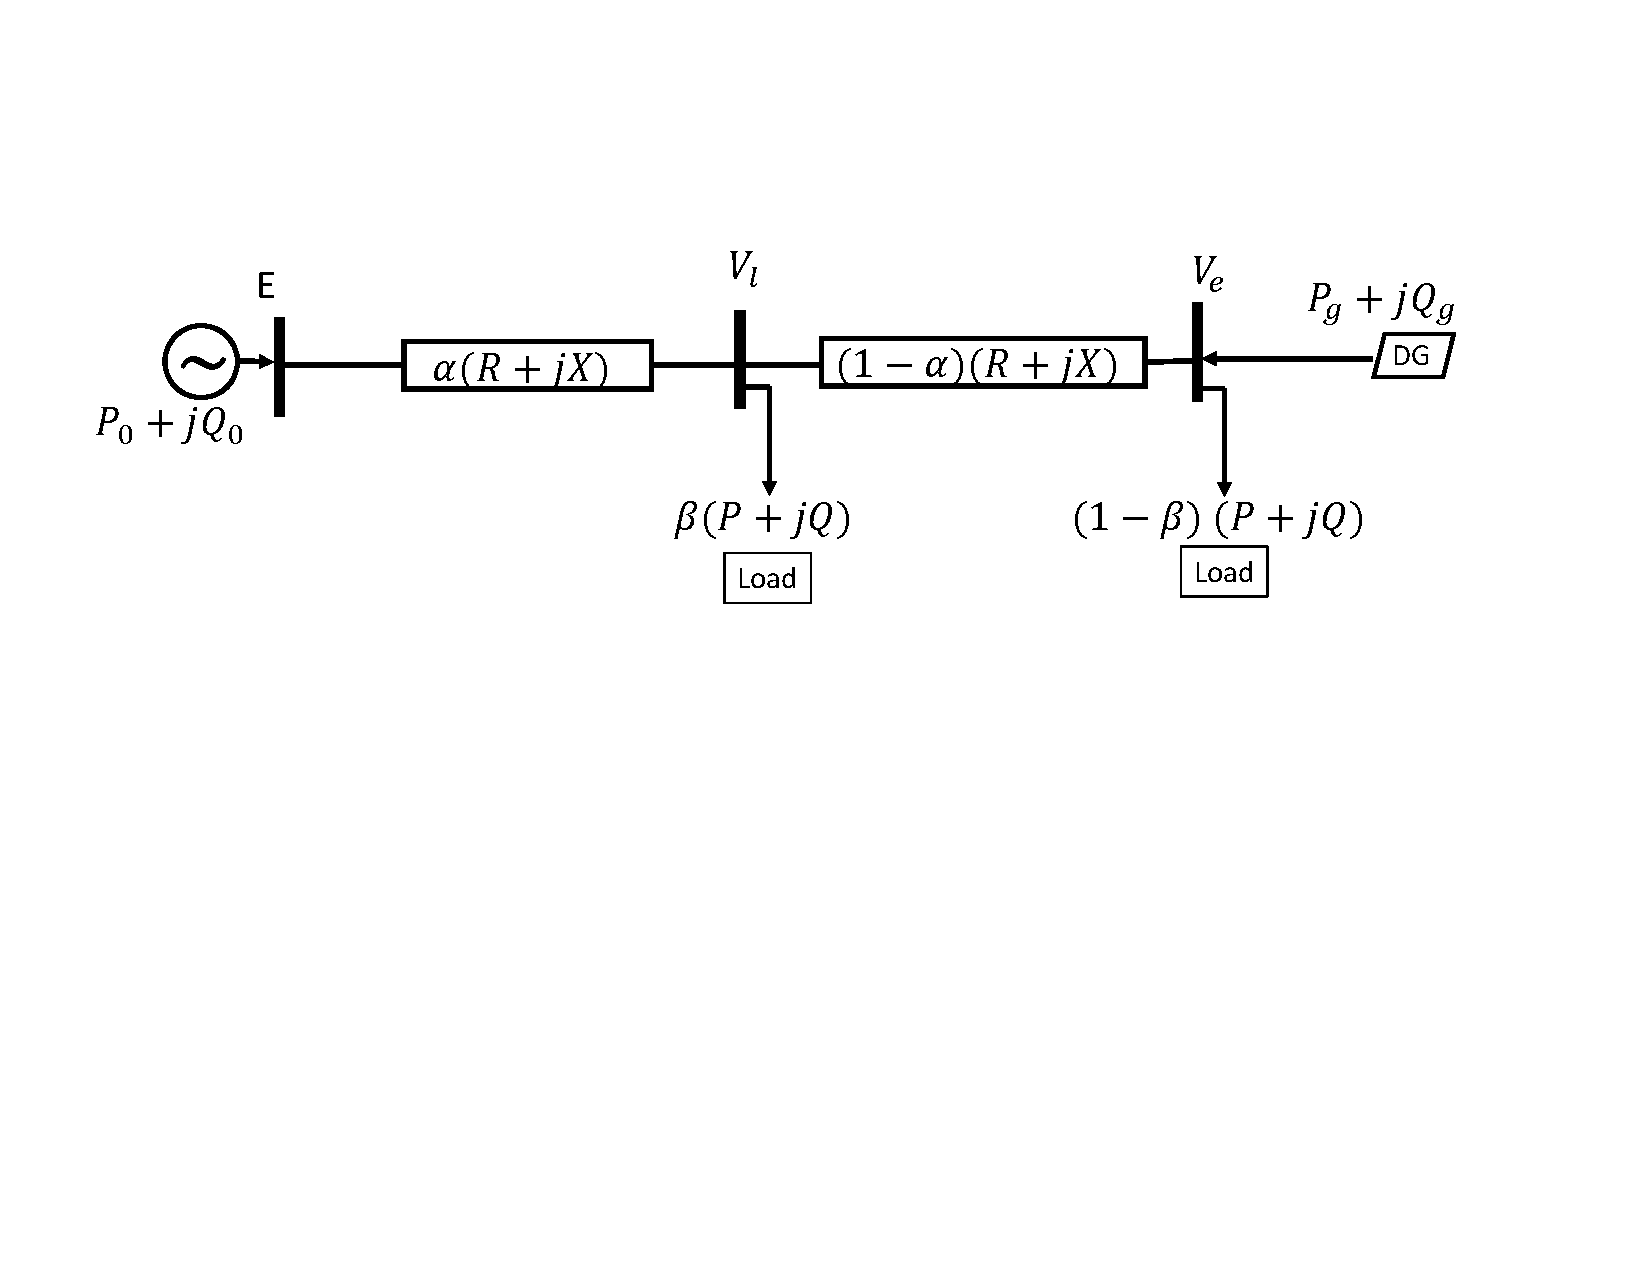
\includegraphics[width=\linewidth]{pics/Lcase.pdf}
    \caption{Illustration system of distribution network with high penetration renewables}
    \label{fig:3bussys}
\end{figure}
In the system, $E$, $V_l$ and $V_e$ are bus voltages; $P_0+jQ_0$ is the power at the feeder; the total generation is represented by $P_g+jQ_g$ as an aggregated DG; the synthetic electrical line between aggregated DG and substation is assumed to be $R+jX$; the total load is denoted by $P+jQ$.
The parameter $\alpha\in [0,1]$ is used to denote the position of the load bus, and $\beta\in[0,1]$ is an additional parameter to split the load between two buses. Also define the the losses by $P_{L_1}+jQ_{L_1}$ and $P_{L_2}+jQ_{L_2}$ for the two line segments ($E$,$V_l$) and ($V_l$,$V_e$), respectively.
%\begin{equation}
    
%\end{equation}

It follows \eqref{eq:brchflowvpl} that,
\begin{align*}
E^2-V_l^2  &=2\alpha RP+2\alpha X Q-2\alpha RP_g-2\alpha X Q_g \\
&+\alpha RP_{L_1}+2\alpha RP_{L_2}+\alpha X Q_{L_1}+2\alpha XQ_{L_2},\\
E^2-V_e^2&=2(\alpha\beta+1-\beta)RP+2(\alpha\beta+1-\beta)X Q \\
&+
\alpha RP_{L_1}+(1+\alpha) RP_{L_2}+\alpha X Q_{L_1}+(1+\alpha) XQ_{L_2},
\end{align*}
and
\begin{align*}
P_{L_1} &=\frac{\alpha R}{V_l^2}\left(\left[P-P_{g}+P_{L_2}\right]^2+\left[Q-Q_{g}+Q_{L_2}\right]^2 \right), \\
P_{L_2} &= \frac{(1-\alpha)R}{V_e^2}\left(\left[(1-\beta)P-P_{g}\right]^2+\left[(1-\beta)Q-Q_{g}\right]^2 \right),
\end{align*}
where
\begin{align*}
Q_{L_1}=\frac{P_{L_1}X}{R} \text{ and } Q_{L_2}=\frac{P_{L_2}X}{R}.
\end{align*}
Given the voltage at feeder $E$, the four variables, $V_e$, $V_l$, $P_{L_1}$ and $P_{L_2}$ can be solved from the above four equations. The voltage $V_e$ and the total loss $P_{L_1}+P_{L_2}$ with respect to DG injection are shown in Figure \ref{fig:ve} and \ref{fig:loss}, respectively.

\begin{figure}[h]
\centering
    \subfloat[bus voltage]{
         %\centering
         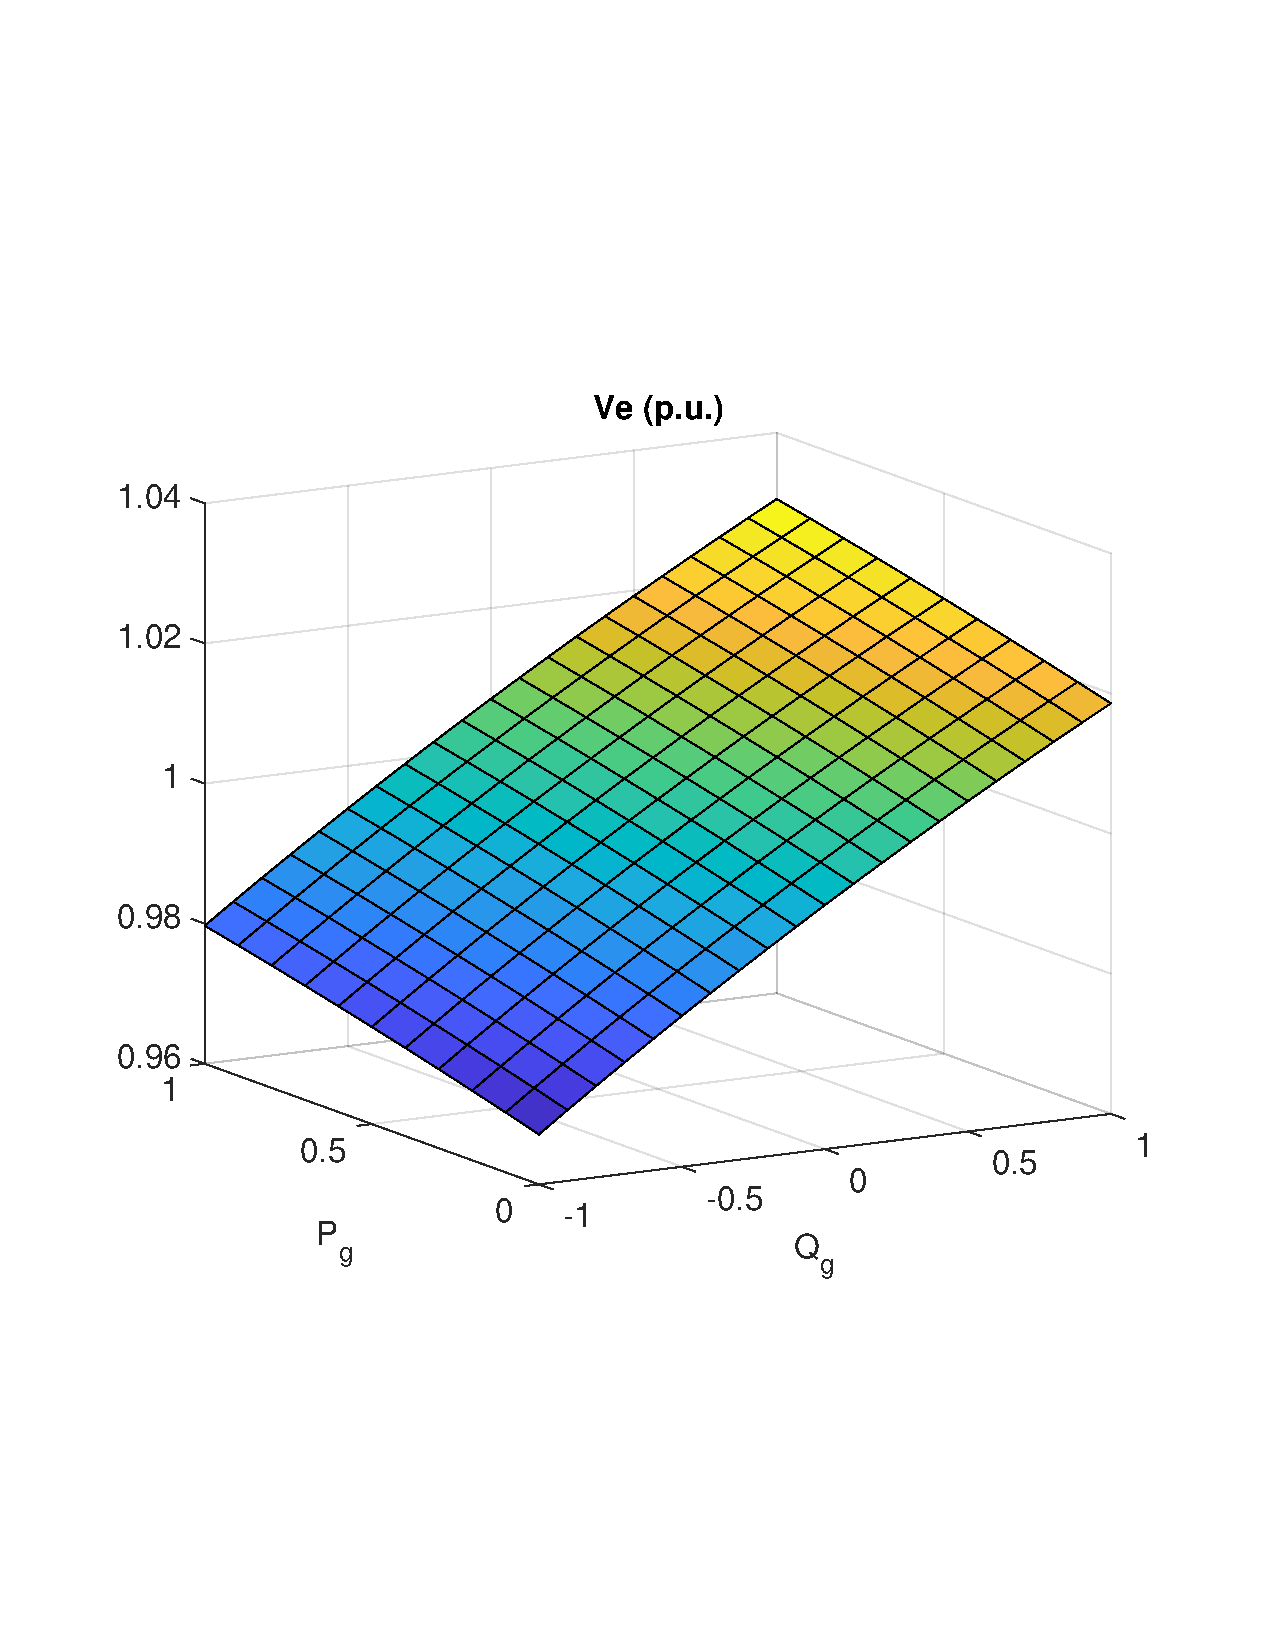
\includegraphics[width=0.46\linewidth]{pics/v_e.pdf}
         \label{fig:ve}
         }
\quad
    \subfloat[system loss]{
        % \centering
         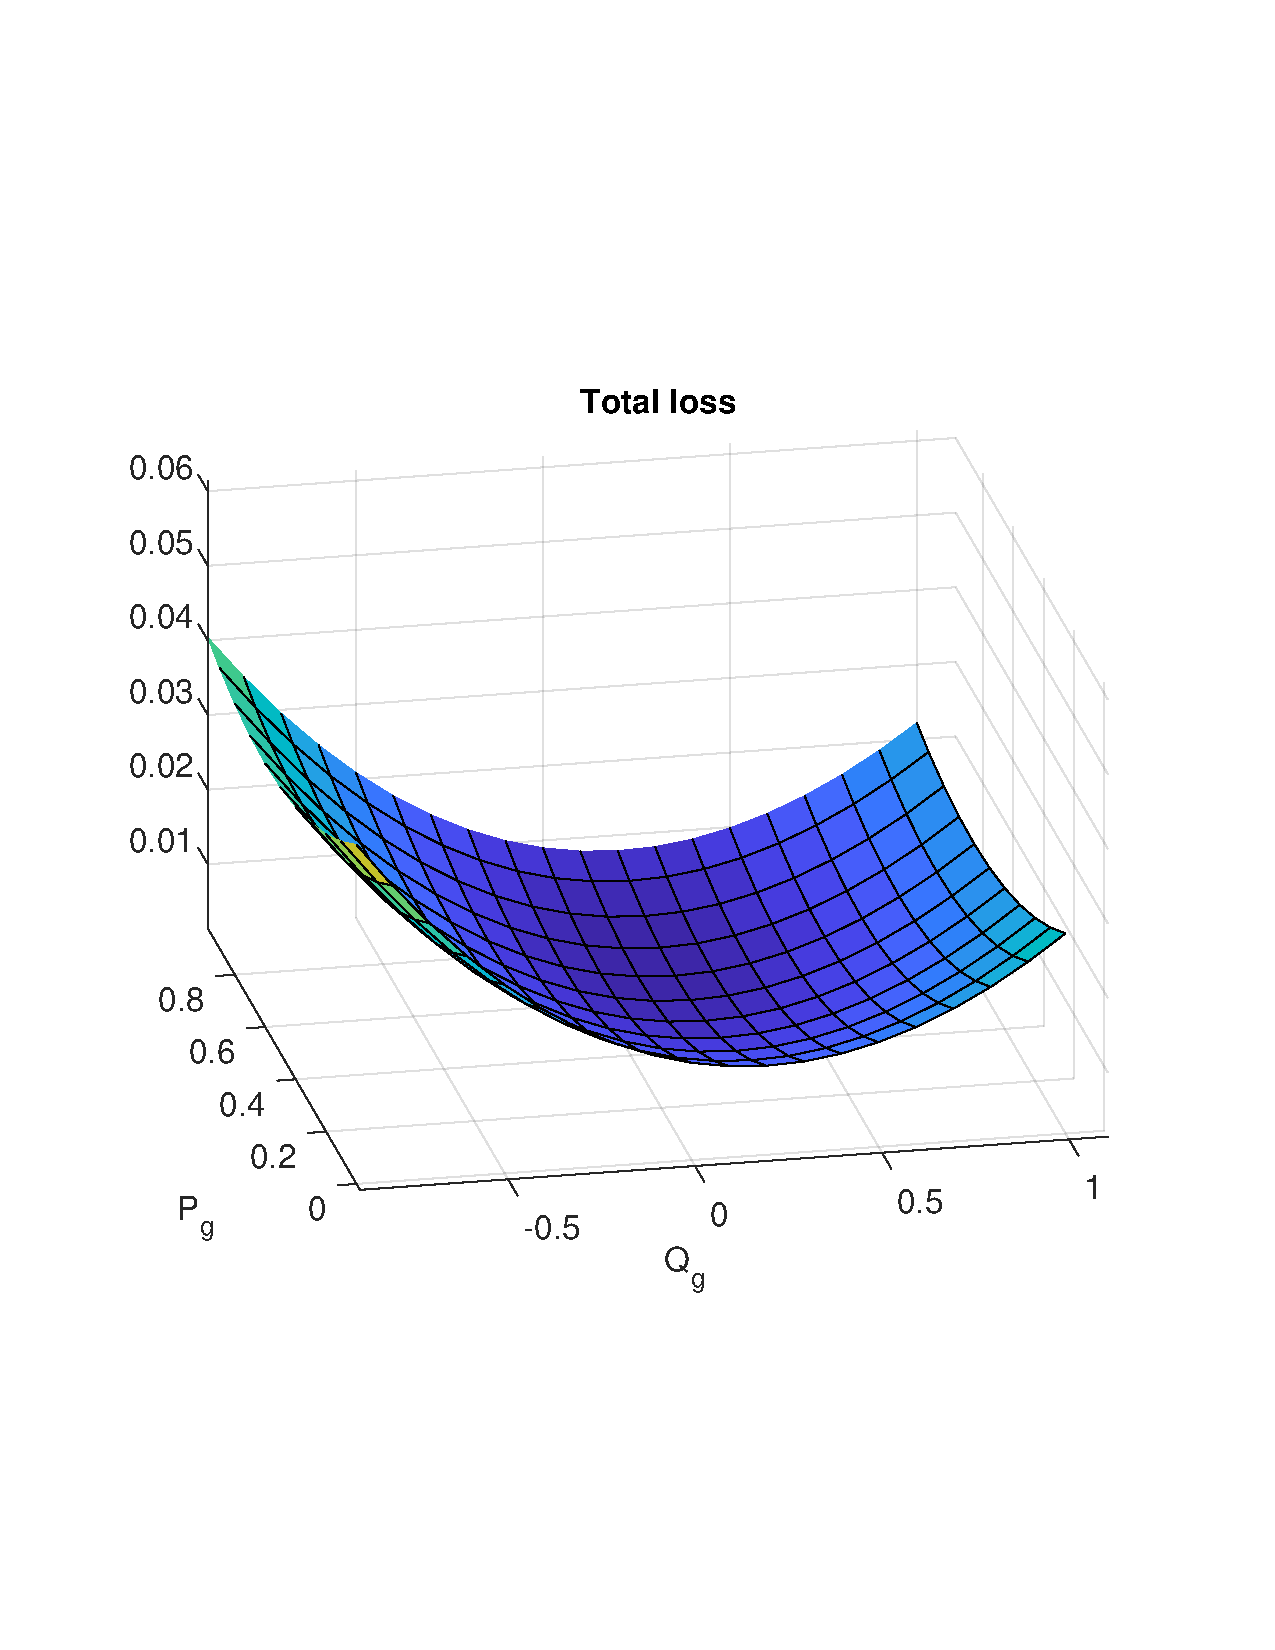
\includegraphics[width=0.46\linewidth]{pics/loss.pdf}
        \label{fig:loss}
         }
    \caption{Bus voltage and system loss with respect to power injection from DGs} 
    \label{fig:phsor_diagram}
\end{figure}


The above results show that system voltage is monotonic to bus power injection \cite{miu2000existence}, and system loss is convex when bus injections are near normal operational points \cite{gan2016online}. These two properties are very useful to the control design of large-scale distribution network with high-penetration of renewables.

By Kirchhoff law, the power at the feeder is then calculated by
\begin{align*}
&P_0 = P-P_{g}+P_{L_1}+P_{L_2},\\
&Q_0 = Q-Q_{g}+Q_{L_1}+Q_{L_2}.
\end{align*}
To compensate the power factor at the feeder, the reactive power support required at the substation can be calculation by
\begin{equation}
    Q_{bank} \overset{\Delta}{=} Q_0 - P_0\sqrt{\left(\frac{1}{pf}\right)-1}
\end{equation}


\begin{figure}[h]
\centering
    \subfloat[$Q_{bank}$]{
         %\centering
         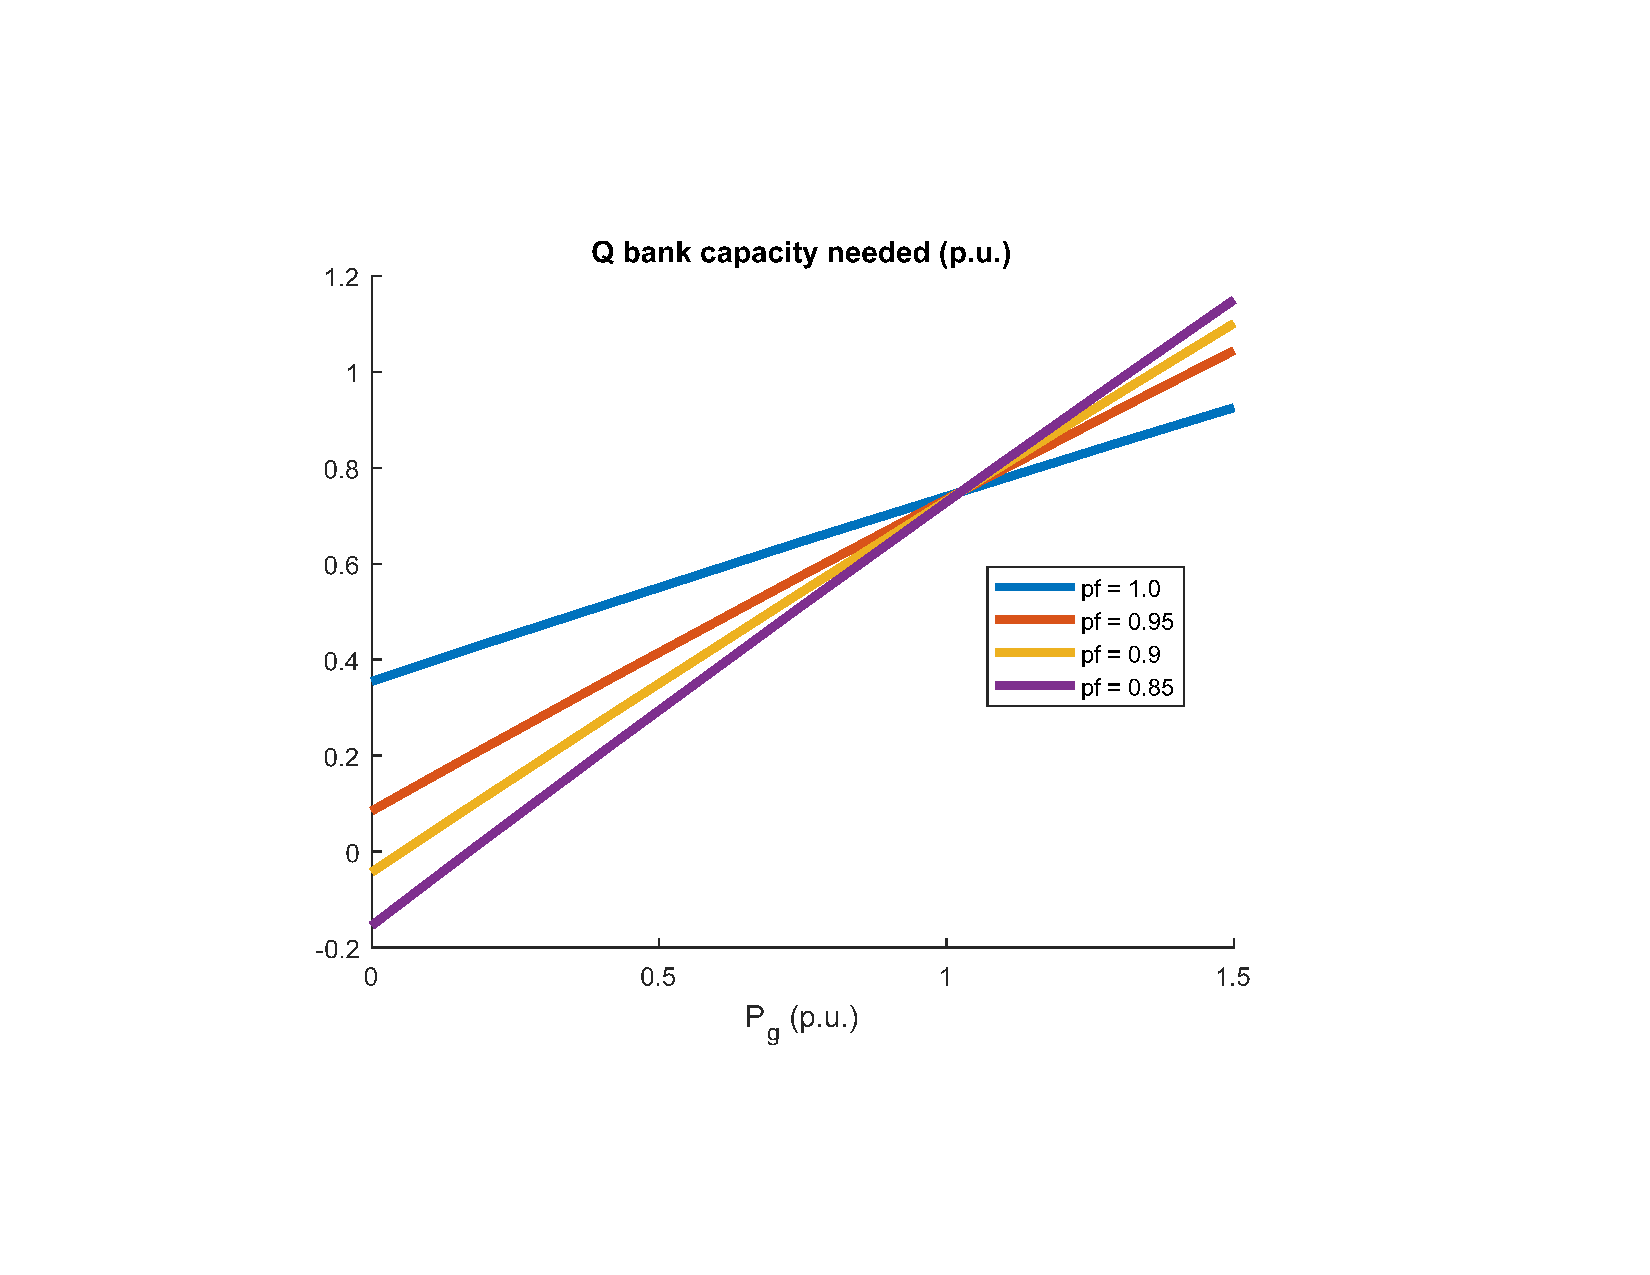
\includegraphics[width=0.46\linewidth]{pics/qbank.pdf}
        \label{fig:qbank}
         }
\quad
    \subfloat[$Q_0$]{
        % \centering
         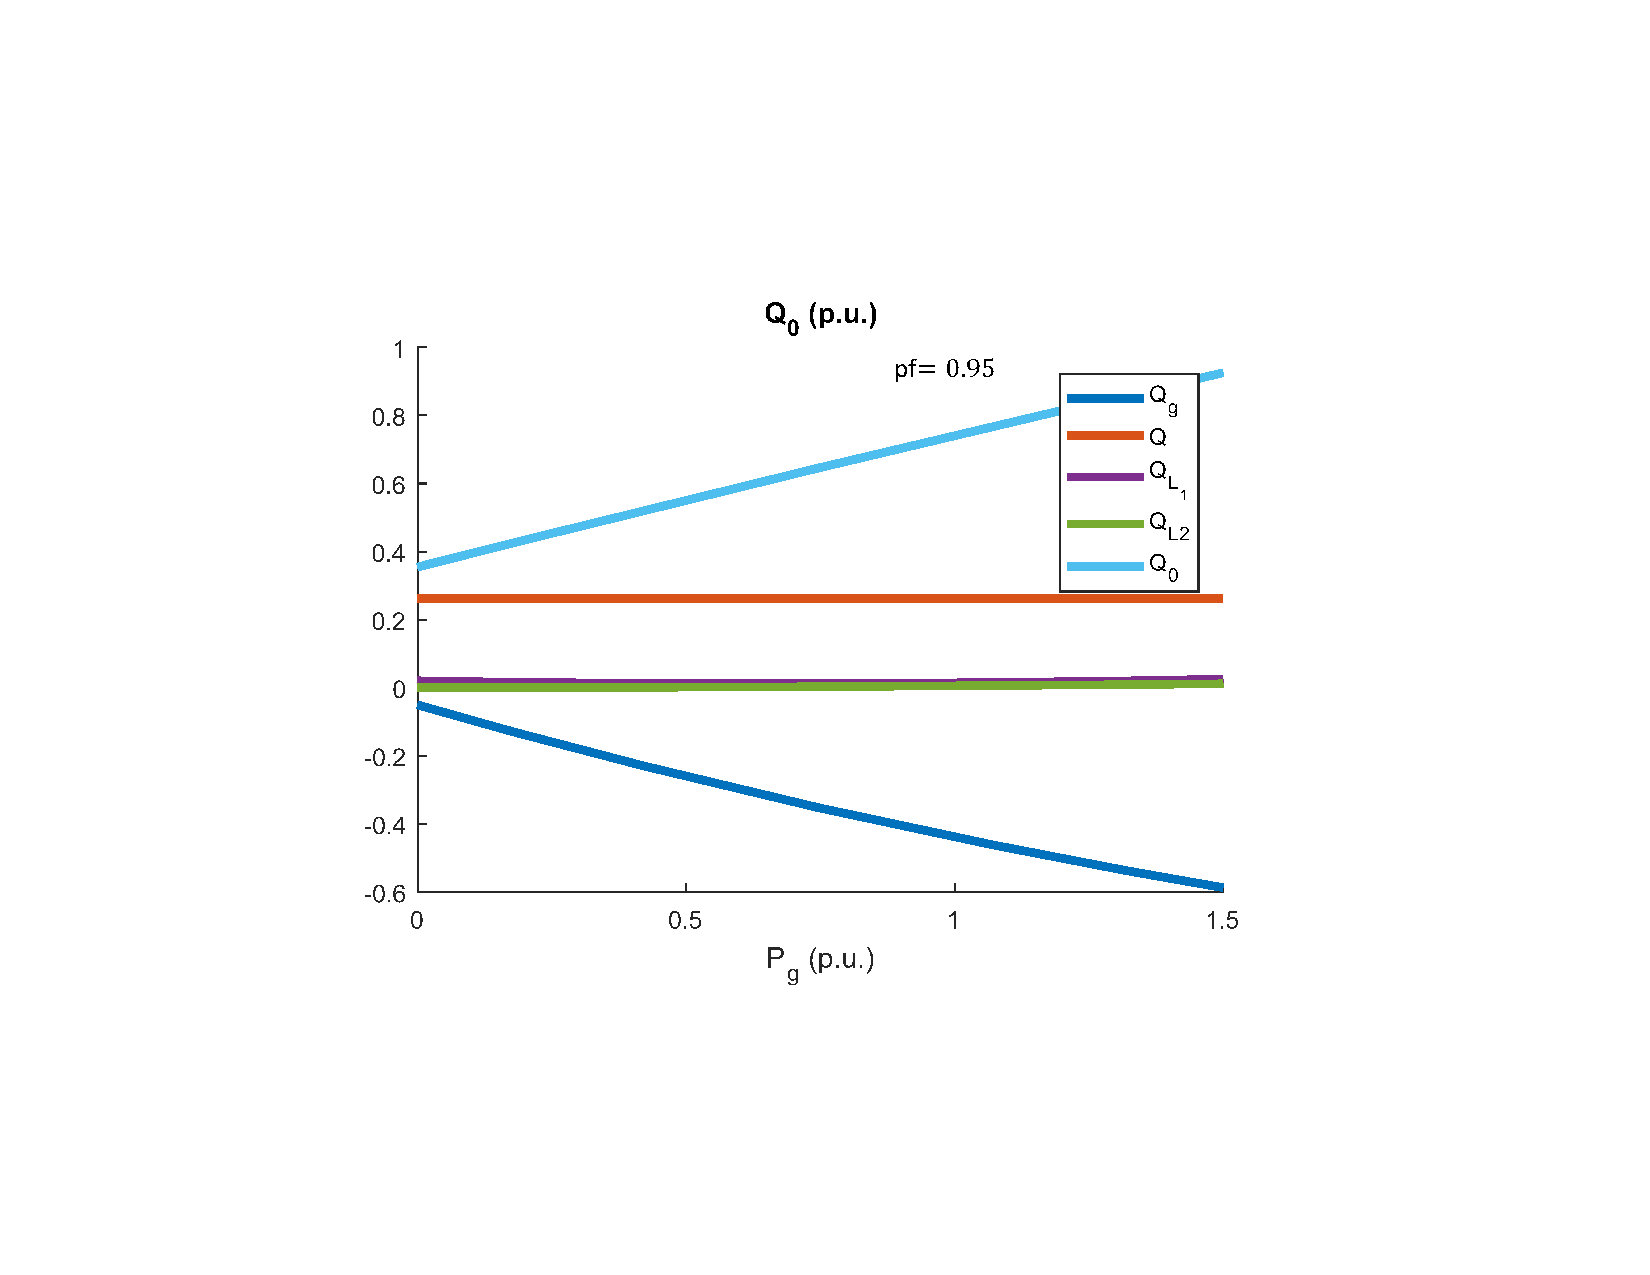
\includegraphics[width=0.46\linewidth]{pics/q0.pdf}
        \label{fig:q0}
         }
    \caption{Reactive power support at the feeder with respect to power injection from DGs} 
    \label{fig:q0qbank}
\end{figure}
The results of $Q_{bank}$ and $Q_0$ are shown in Figure \ref{fig:q0qbank}. As shown in Figure \ref{fig:q0}, it is clear that the reactive power of DG ($Q_g$) increases (absorption) along with the increase of its real power ($P_g$), which is close to a linear relationship, as described in \eqref{eq:vkliniear}, given relatively small line loss. This is also true for $Q_0$ and $Q_{bank}$. The necessary reactive power support is also studied with different $\alpha$ and $\beta$ (different load conditions), and results are shown in Figure \ref{fig:qalfa} and \ref{fig:qbeta}.
\begin{figure}[h]
\centering
    \subfloat[$Q_{bank}$ under different $\alpha$]{
         %\centering
         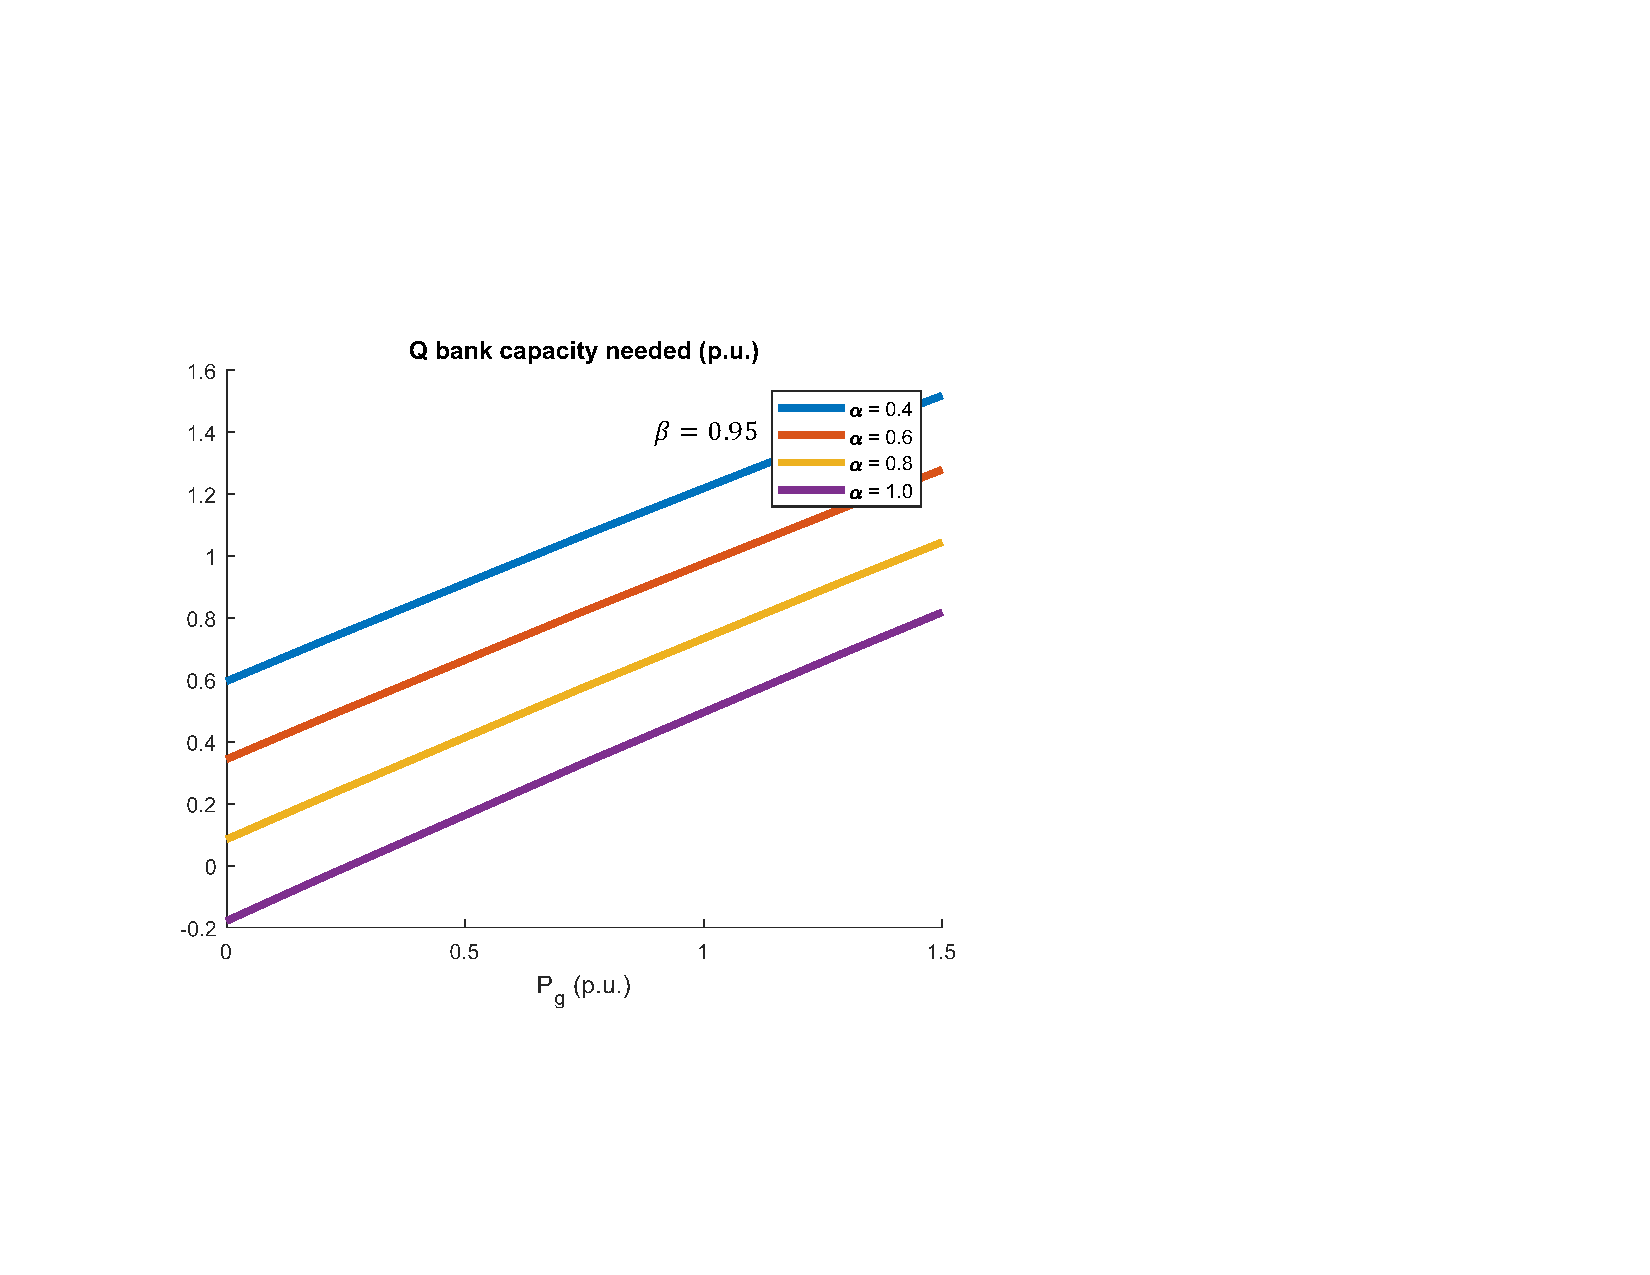
\includegraphics[width=0.46\linewidth]{pics/qalfa.pdf}
        \label{fig:qalfa}
         }
\quad
    \subfloat[$Q_{bank}$ under different $\beta$]{
        % \centering
         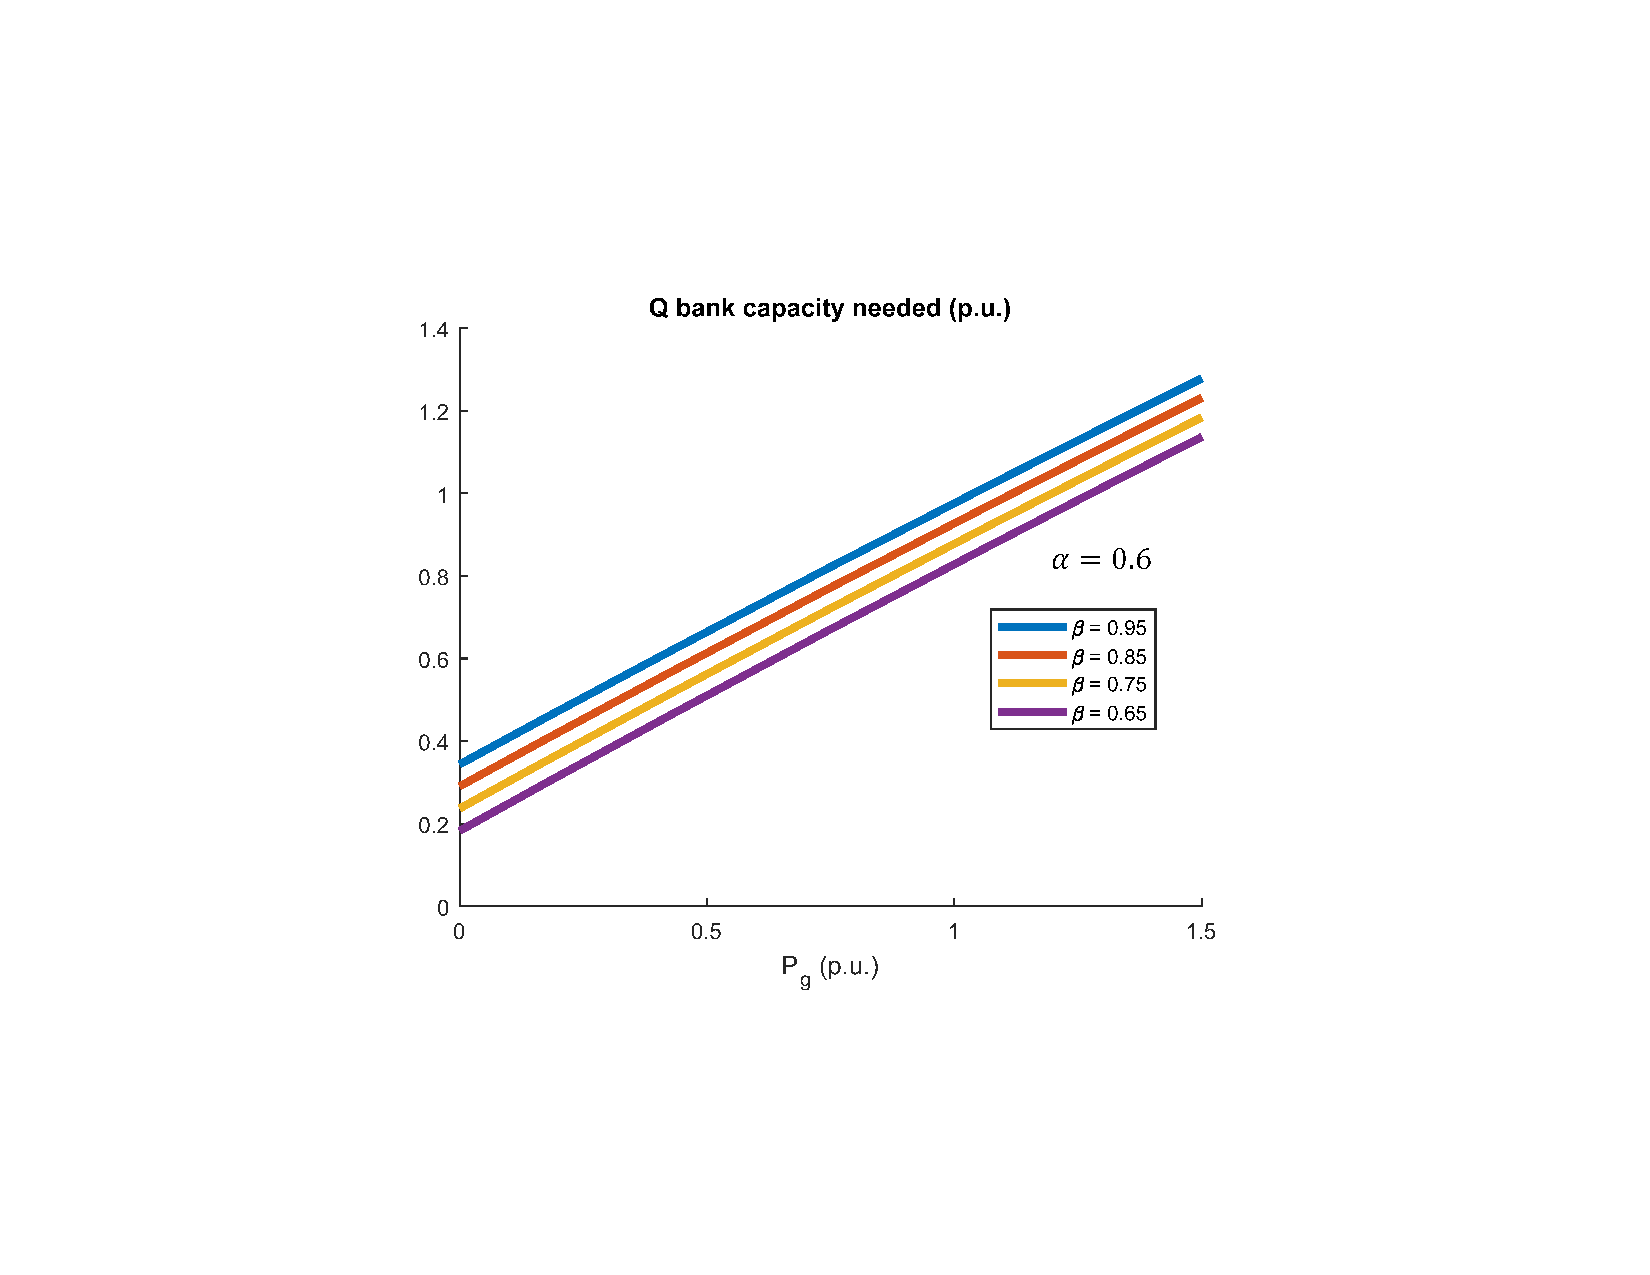
\includegraphics[width=0.46\linewidth]{pics/qbeta.pdf}
        \label{fig:qbeta}
         }
    \caption{Reactive power support at the feeder with respect to power injection from DGs under different load conditions} 
    \label{fig:qbankab}
\end{figure}

\begin{note}
The above equivalent model of an feeder is useful to analyze certain properties of distribution network, such as: reactive power schedule on transmission side, and the network planning. Also, it can be used as heuristic modelling of feeders with less (or no) measurement, T\&D co-simulation and control, etc. 

\end{note}

\section{Hierarchical multi-agent control of large-scale distribution system}\label{sec:syslvl}
The layered and divisional {\bf principle} for large-scale power system planning, operation and control has been practiced for years:
\begin{principal}\label{principal}
For large-scale power system operation:
\begin{enumerate}
    \item Voltage/Var control should be designed as local control, which is within certain electrical or geological area to prevent the transfer of reactive power, and to avoid unnecessary losses;
    \item Real power control should respond to system-level objectives such as: frequency regulation, operation optimization, etc.;
\end{enumerate}
\end{principal}

By following the above operation principal, an hierarchical control is presented, as shown in Figure \ref{fig:hrchy}. In the hierarchy, voltage control is considered as a local problem within an electrical or geological area while real power control (frequency control) is formulated as global problem. Accordingly, the communication network is organized as either local or wide-area network. 
\begin{figure}
    \centering
    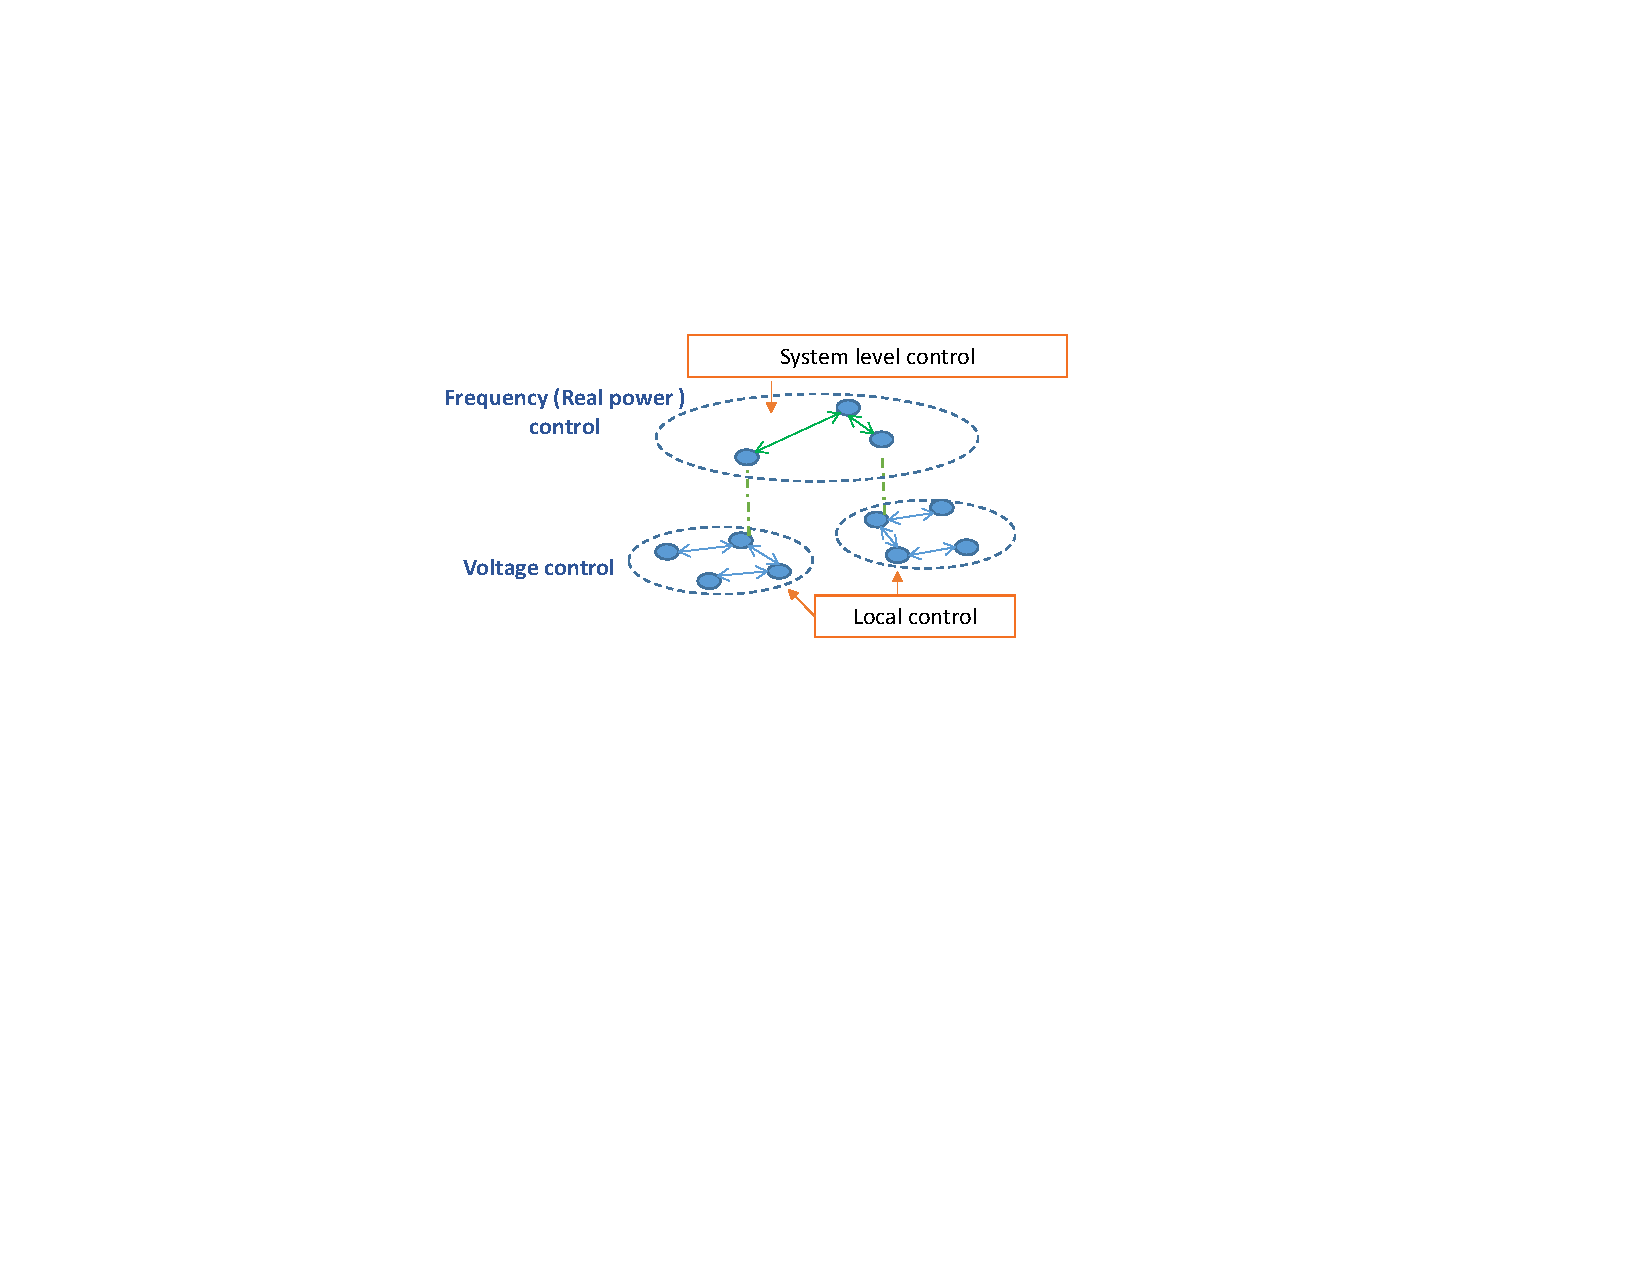
\includegraphics[width=\linewidth]{pics/hierarchy.pdf}
    \caption{Hierarchical control design for voltage and frequency control}
    \label{fig:hrchy}
\end{figure}
We define each local area as a cluster and each bus (or each information agent) as a node. 
We assign a virtual leader (VL) in each cluster which is the connection between the two layers: it works as virtual node in local cluster and an aggregated agent for the upper-level control, as shown in Figure \ref{fig:hrchy}.

We expand the denotations to fit the hierarchy as follows:
$\mathcal{G}^{L}$ is the set of all VLs in all clusters; $\mathcal{N}^{k}$ is the set of all nodes in the $k^{th}$ cluster, $k\in\mathcal{G}^{L}$; $0$ is a default member of all $\mathcal{N}^{k}$s, which means the subscript $0$ is specified for variables of VL node within each cluser, e.g. $P_{g_0}$ and $Q_{g_0}$ are used to denote the power output of VLs. Then we can redefine the communication matrix \eqref{eq:comms} for each cluster with its augmented form as follow:

\begin{equation}
S = \left[
\begin{array}{cccc}
s_{00}(t)&s_{01}(t)&\cdots & s_{0n}(t);\\
s_{10}(t)&s_{11}(t)&\cdots & s_{1n}(t);\\
 \vdots&  \ddots&\cdots &\vdots \\
s_{n0}(t)&\cdots&\cdots &s_{nn}(t)
\end{array}
\right],\label{eq:commsp}
\end{equation}
where $s_{ij} = 1$ if $j \in N_i^c$, otherwise $s_{ij} = 0$; and $d_{ij}$ is redefined in the same way as in \eqref{eq:dij} for all $i,j \in \mathcal{N}^k$.

\subsection{Virtual leader design}
The properties of VLs are specified by a superscript $L$ and being defined as follows: $\overline P^L_k$ and $\overline Q^L_k$ are defined to collect the capacities of all DGs within the $k^{th}$ cluster, i.e.

\begin{equation}
    \overline P^L_{g_k}=\sum_{j\in \mathcal{N}^{k}}\overline P_{g_j},\;\;\overline Q^L_{g_k}=\sum_{j\in \mathcal{N}^{k}}\overline Q_{g_j},\;\;k\in \mathcal{G}^{L}; \label{eq:vlpq}
\end{equation}
$\alpha^L_{p_k}$ and $\alpha^L_{q_k}$ are defined as utilization ratios of the $k^{th}$ cluster. For simplicity of expression, in the context of local control within the $k^{th}$ cluster, $\alpha^L_{p_k}$ and $\alpha^L_{q_k}$ are represented as $\alpha_{p_0}$ and $\alpha_{q_0}$ respectively. 

\begin{figure}[ht]
    \centering
    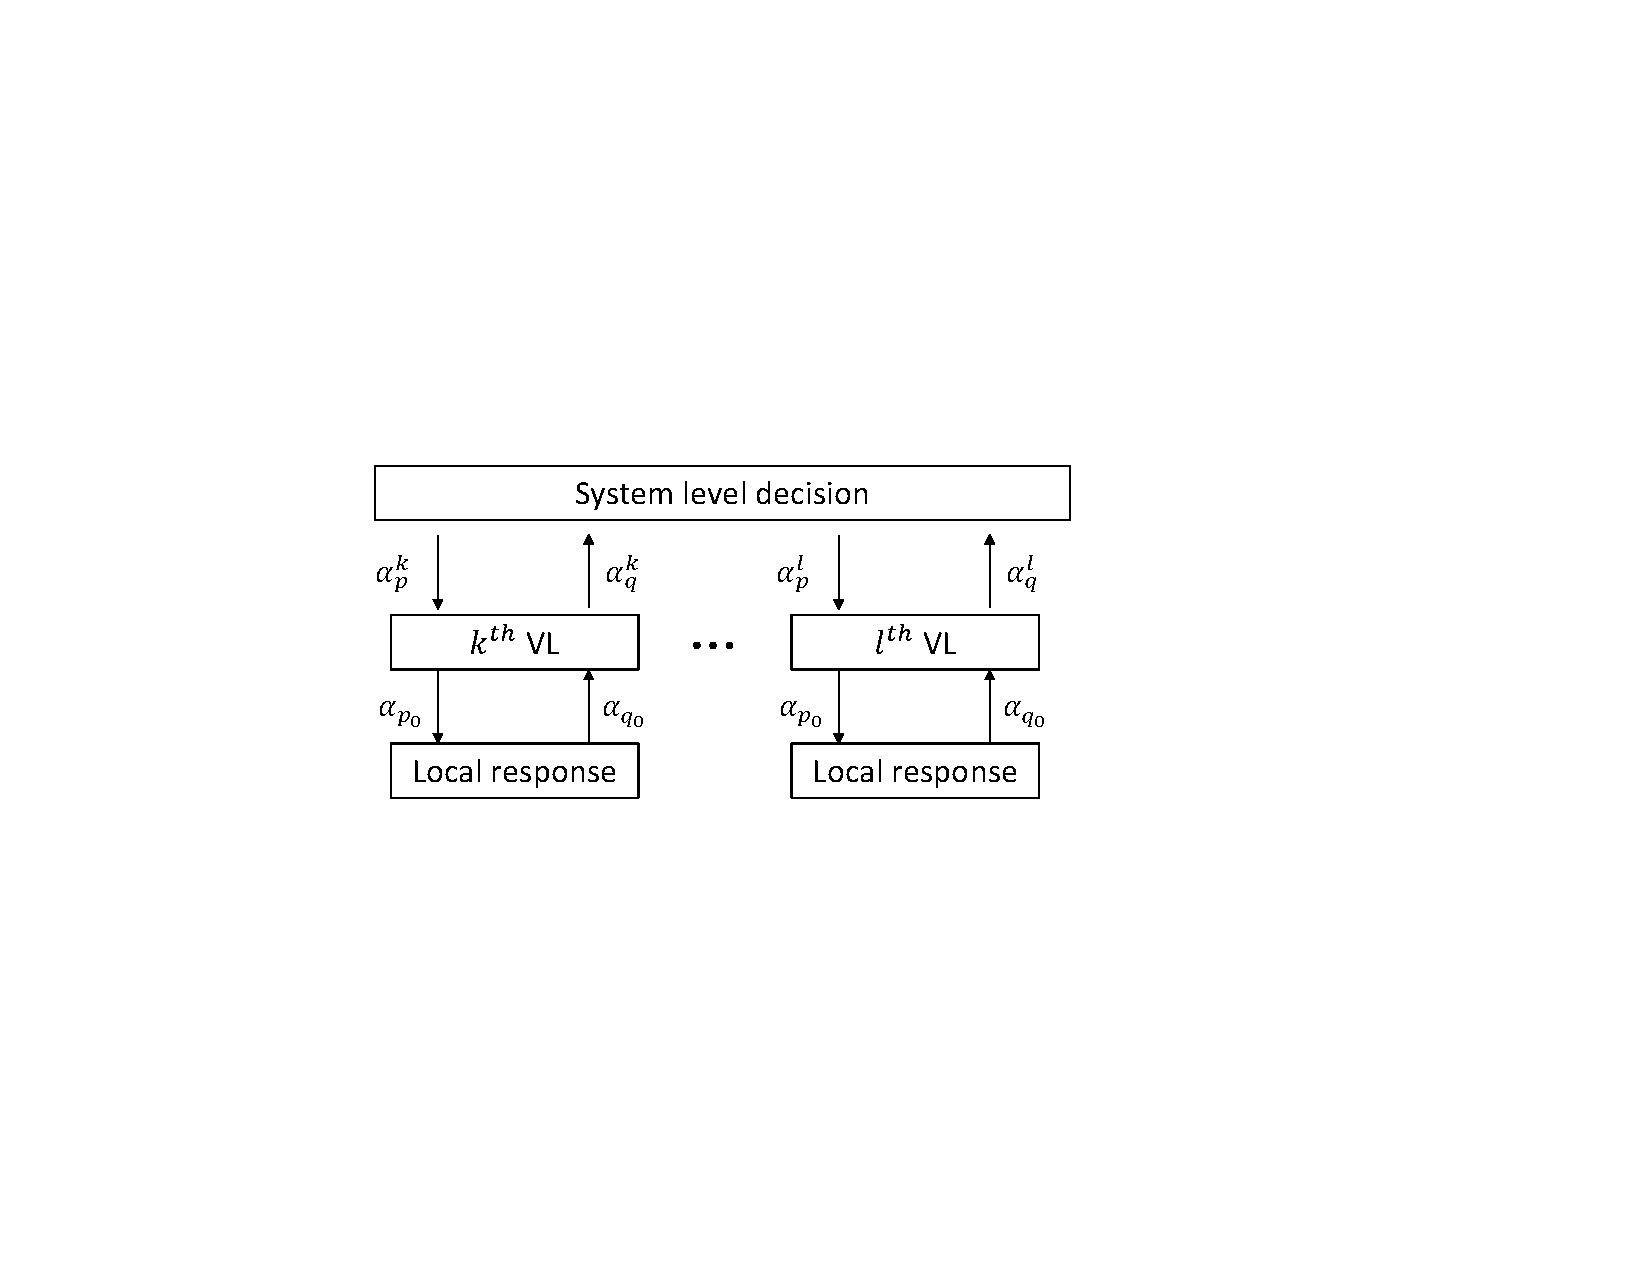
\includegraphics[width = 8cm]{pics/ctrl_strc.pdf}
    \caption{Information flow of the hierarchical control}
    \label{fig:ctrl_strc}
\end{figure}

The computational sequences in the hierarchy are shown in the information flow in Figure \ref{fig:ctrl_strc}: $\alpha_q^k$ is the results of local control hence it is calculated from each cluster by standard cooperative law; while real power $\alpha_p^k$ is on the opposite way, from system level to each of the clusters. 

The real power control aims to pursue system level objectives such as: driving the downstream or upstream power flow at the feeder to follow the dispatch signals from OPF (or control center), optimizing operation in terms of system loss or power quality, and so on. One practival design of control objective for real power, which focuses on the fast response to load demand and voltage regulation, can be written as follow:
\begin{equation}
    f^L_i =
    \frac{\lambda^{Lf}_i}{2}(P_{f}^{*}-P_{f})^2+\frac{\lambda^{Lv}_i}{2}(1-V^L_{i})^2
    ,\;\;i\in \mathcal{G}^L,\label{eq:fif}
\end{equation}
where $\lambda_i^{Lf}\geq 0$ and $\lambda^{Lv}_i\geq 0$ are the coordinate coefficients at the $i^{th}$ agent; $P_{f}$ and $P_{f}^{*}$ denotes the power at the feeder of distribution systems and its dispatch value, respectively; $V^L_{i}$ is the representative voltage of the cluster, particularly, the worst measured voltage of the cluster.
$\lambda_i^{Lf}$ is impact factor of frequency or power dispatch control for main grid (transmission side), which should be zeros when the distribution system is isolated from main grid. 

Let's define $z_{ik}$ as the estimation of $P^{*}_{g_k}$ at the $i^{th}$ agent. As described by Figure \ref{fig:ctrl_strc}, reactive power is not considered as decision variable at system level. 
We follow \cite{gan2016online} to make the assumption that $\frac{\lambda^{Lf}_i}{2}(P_{f}^{*}-P_{f})^2$ is convex in the context of normal power system operation. Hence \eqref{eq:fif} is convex and the distributed subgradient control \eqref{eq:ccl} is also deployed on system level.
Then distributed subgradient law \eqref{eq:ccl} can be used, and we have
\begin{equation}
    \dot z_{ik} = \sum_{j\in N_i^c}d_{ij} (z_{jk}-z_{ik})-\beta_ig_{ik},\label{eq:cclz}
\end{equation}
where $g_{ik}$ is the gradient of $f^L_i$ with respect to $z_i$ which can be written as
\begin{equation}
 \begin{split}
g_{ik}=\lambda^f_i(P_f-P^*_f)\frac{\partial p_{f}}{\partial p_{g_k}}+\lambda^v_i( V_i-1)\frac{\partial V_i}{\partial P_{g_k}}.
 \end{split}   \label{eq:gik}
\end{equation}

\begin{note}
Different from local subgradient calculation at lower level, the standard subgradient calculation requires information across the system to pursue the optimal operation point on the system level ($\frac{\partial V_i}{\partial P_{g_k}}$). However, the computation should not be too large for reasonably planned systems because only the clusters that can not control the voltage by themselves need the subgradients calculation.
\end{note}

According to the hierarchy design, the voltage control term in \eqref{eq:gik} is a supplementary control and will only be performed when the local reactive power control is not enough. So $\frac{\partial V_i}{\partial P_{g_k}}=0$ when $i=k$ because the local voltage control has already been considered at the lower level. When $i\neq k$, the supplementary voltage control is needed and hence calculation of $\frac{\partial V_i}{\partial P_{g_k}}$ is performed only under the following conditions: 
\begin{enumerate}[label=C\arabic*]
    \item: $\alpha^i_{q}$ (or $\alpha_{q_0}$ in the $i^{th}$ cluster) has reached its limit;
    \item: $V_i$ violates the regulation limits;\label{c2}
    \item: $V_k$ is well controlled within the regulation limits.\label{c3}
\end{enumerate}

The condition \ref{c3} implies that the reactive power at the $k^{th}$ cluster is sufficient to maintain the local voltage within that cluster, and the reactive power control is a fast response to change of $P_k$ given $V_k$ being well controlled. So we can estimate the reactive power response at VLs, and use \eqref{eq:vkliniear} to approximate the derivative of $Q_k$ to $P_k$ i.e. $-{\mathcal{R}_{kk}}/{\mathcal{X}_{kk}}$. We refer to branch power flow model \eqref{eq:brchflowvpl}, condition \ref{c3}, and through derivation we can get the following results:
\begin{equation}
\begin{split}
    \frac{\partial V_i}{\partial P_{g_k}} =& \frac{1}{2V_i}(\mathcal{R}_{ik}-\frac{\mathcal{R}_{kk}\mathcal{X}_{ik}}{\mathcal{X}_{kk}})-\sum_{j\in\mathcal {P}_{1k}\cap (\mathcal {P}_{1i}\cup \mathcal{T}_i)} Z'_{kj}\frac{\partial P_{L_j}}{\partial P_{g_k}},\;\;k \in \mathcal{G}^L,
\end{split}\label{eq:dvpl}
\end{equation}
where the derivative of $P_{L_j}$ with respect to $P_{g_k}$ can be calculated from \eqref{eq:brchflow} and \eqref{eq:psqs}, i.e.
\begin{equation}
    \frac{\partial P_{L_j}}{\partial P_{g_k}} =
    \begin{cases}
        -\frac{2R_j}{v_j}\left[P_{S_j}-Q_{S_j}\frac{\mathcal{R}_{kk}}{\mathcal{X}_{kk}}\right]& \text{if }k\in \mathcal{T}_j\\
        0 & \text{if otherwise}         
    \end{cases},\label{eq:dlp}
\end{equation}
where $P_{S_j}$ and $Q_{S_j}$ can be measured. Note that \eqref{eq:dlp} is an approximation made by assuming the impact of both losses in subtree of bus $j$ on $P_{L_j}$ and $\partial P_{L_j}/\partial v_j$ are negligible.

From the above analysis, $z_{ik}$ are consensus variables and the decision variable $P_{g_i}$ should be its estimation at the $i^{th}$ agent, i.e.
\begin{equation}
    P_{g_i} = z_{ii}.
\end{equation}

\subsection{Case study}

IEEE 8500-node system is used to test the proposed hierarchical control on both the system- and cluster- level real/reactive power control. First, we use a case with low voltage problem when only reactive power control is implemented, as shown in Figure \ref{fig:lowvolt}.  
\begin{figure}[ht]
    \centering
\centering
    \subfloat[Circuit]{
    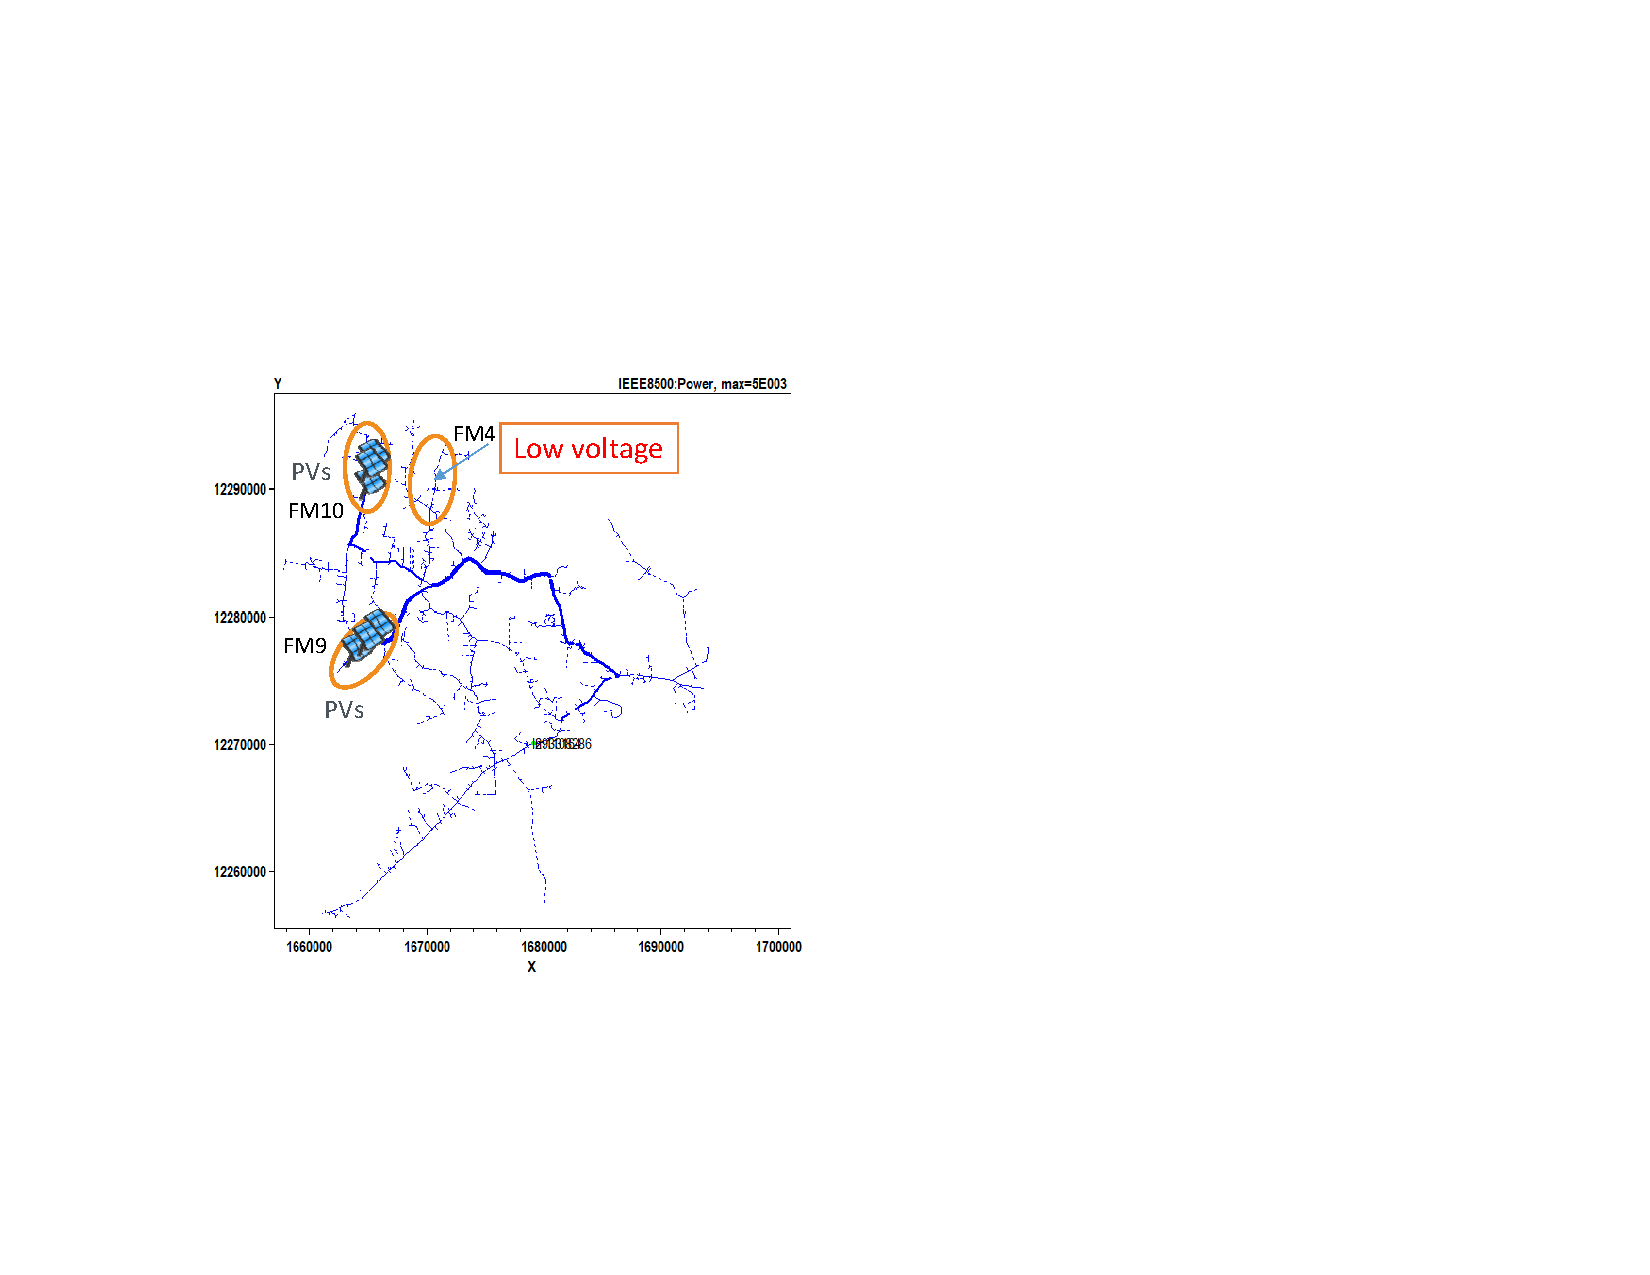
\includegraphics[height=5cm,width=0.45\linewidth]{pics/lowvoltage1.pdf}
    }
    \centering
    \subfloat[Voltage profile]{
    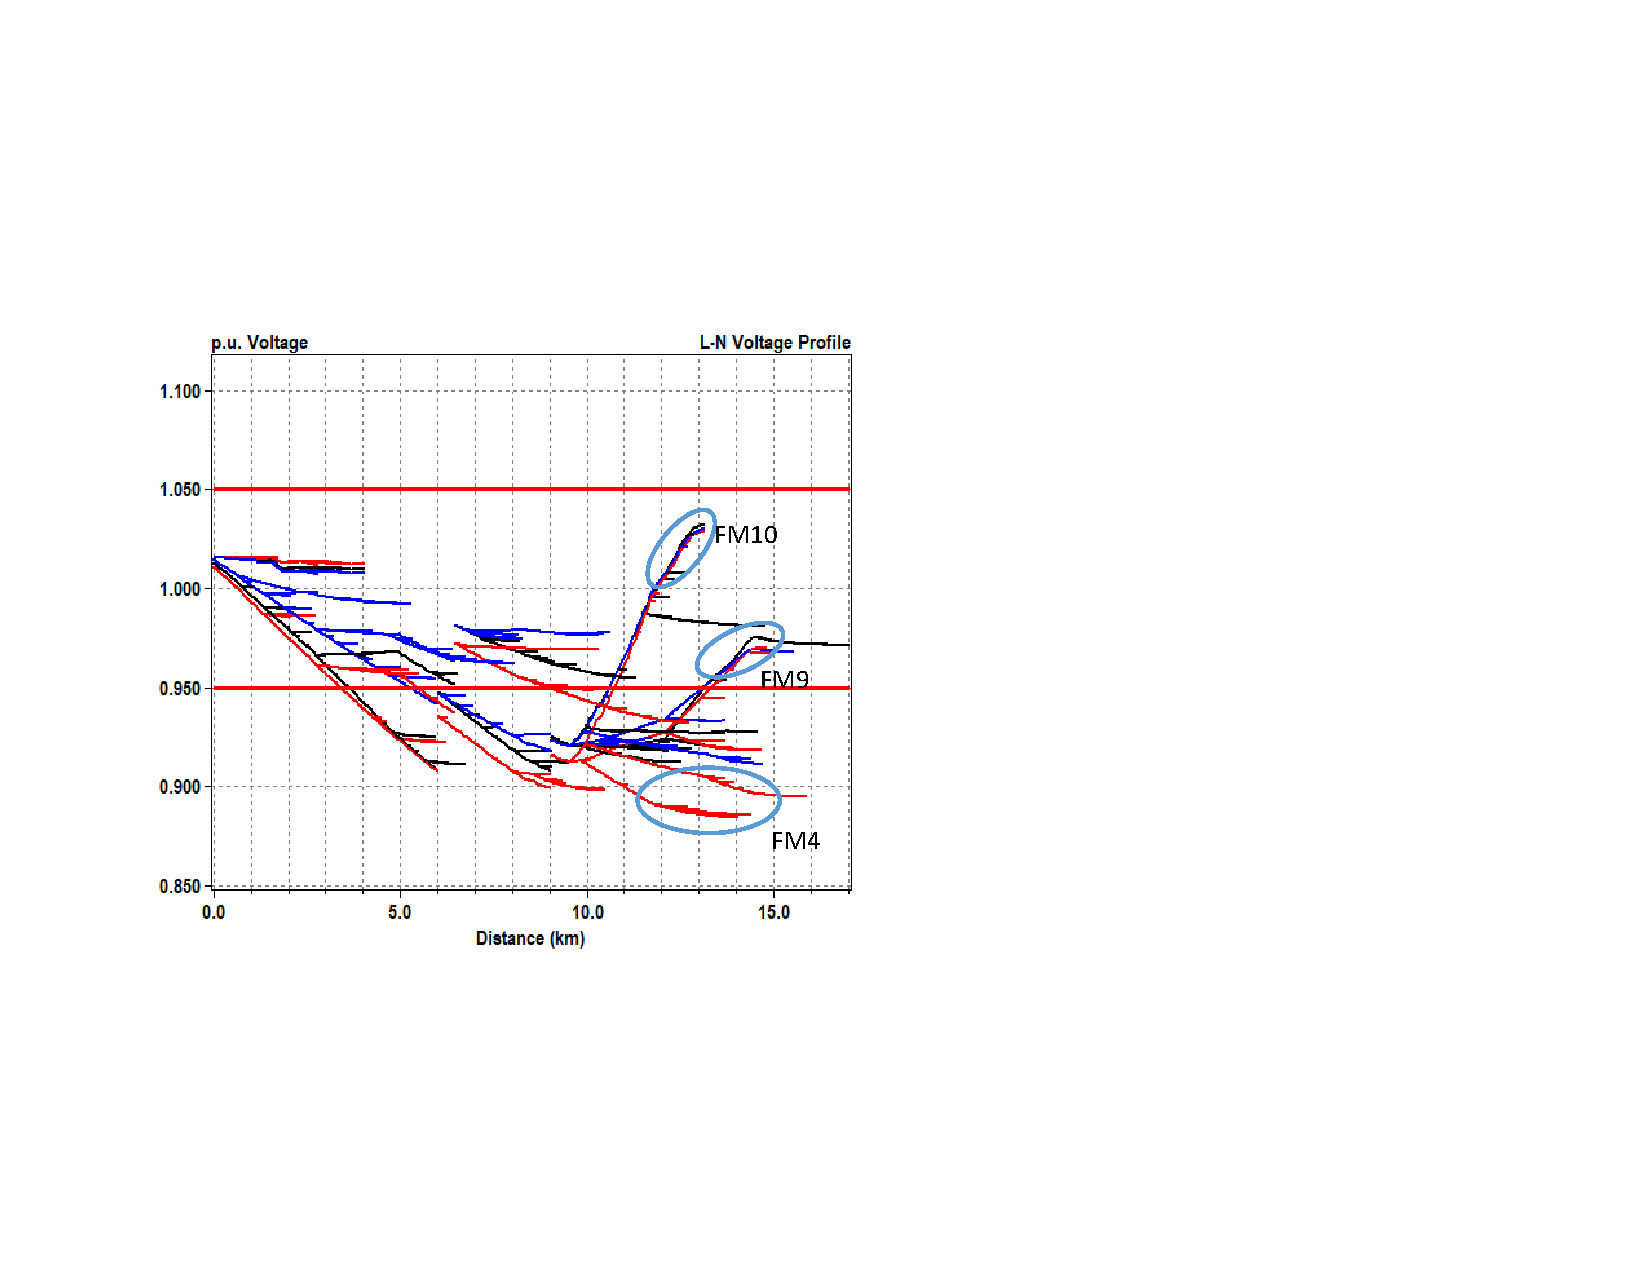
\includegraphics[height=5cm,width=0.45\linewidth]{pics/lowvoltage2.pdf}
    }
    \caption{Low voltage problem due to the spatial unbalance of power flow in IEEE 8500-node system}
    \label{fig:lowvolt}
\end{figure}
The spatial power unbalance in the circuit causes huge voltage deviations between power sources and loads, so it is necessary to implement a system-level control that can work as as supplementary control to fix these problems, especially for large-scale systems. In this case, the area FM4 is experiencing low voltage problem due to the voltage deviations between power sources and loads in the large-scale system. The supplementary control is to compensate the shortfall that the local power control is only for the local voltage.

The control response is shown in Figure \ref{fig:phctrl}. It is shown that the system voltages increase due to the power injection at $t=2s$, then the local reactive power control starts to push the voltage down. At around $t=11s$, the voltage at the lowest bus starts to violate the lower limit of voltage regulation. This is because the local reactive power control is only for the local voltage, which is shown in the second plot of the figure. About the same time, the system-level control starts to kick in and the real power control (curtailment) respond to the system-level objectives. Eventually, the control settles down and all the voltages throughout the network are well controlled.  

\begin{figure}[ht]
    \centering
    \subfloat[Lowest bus voltage]{
    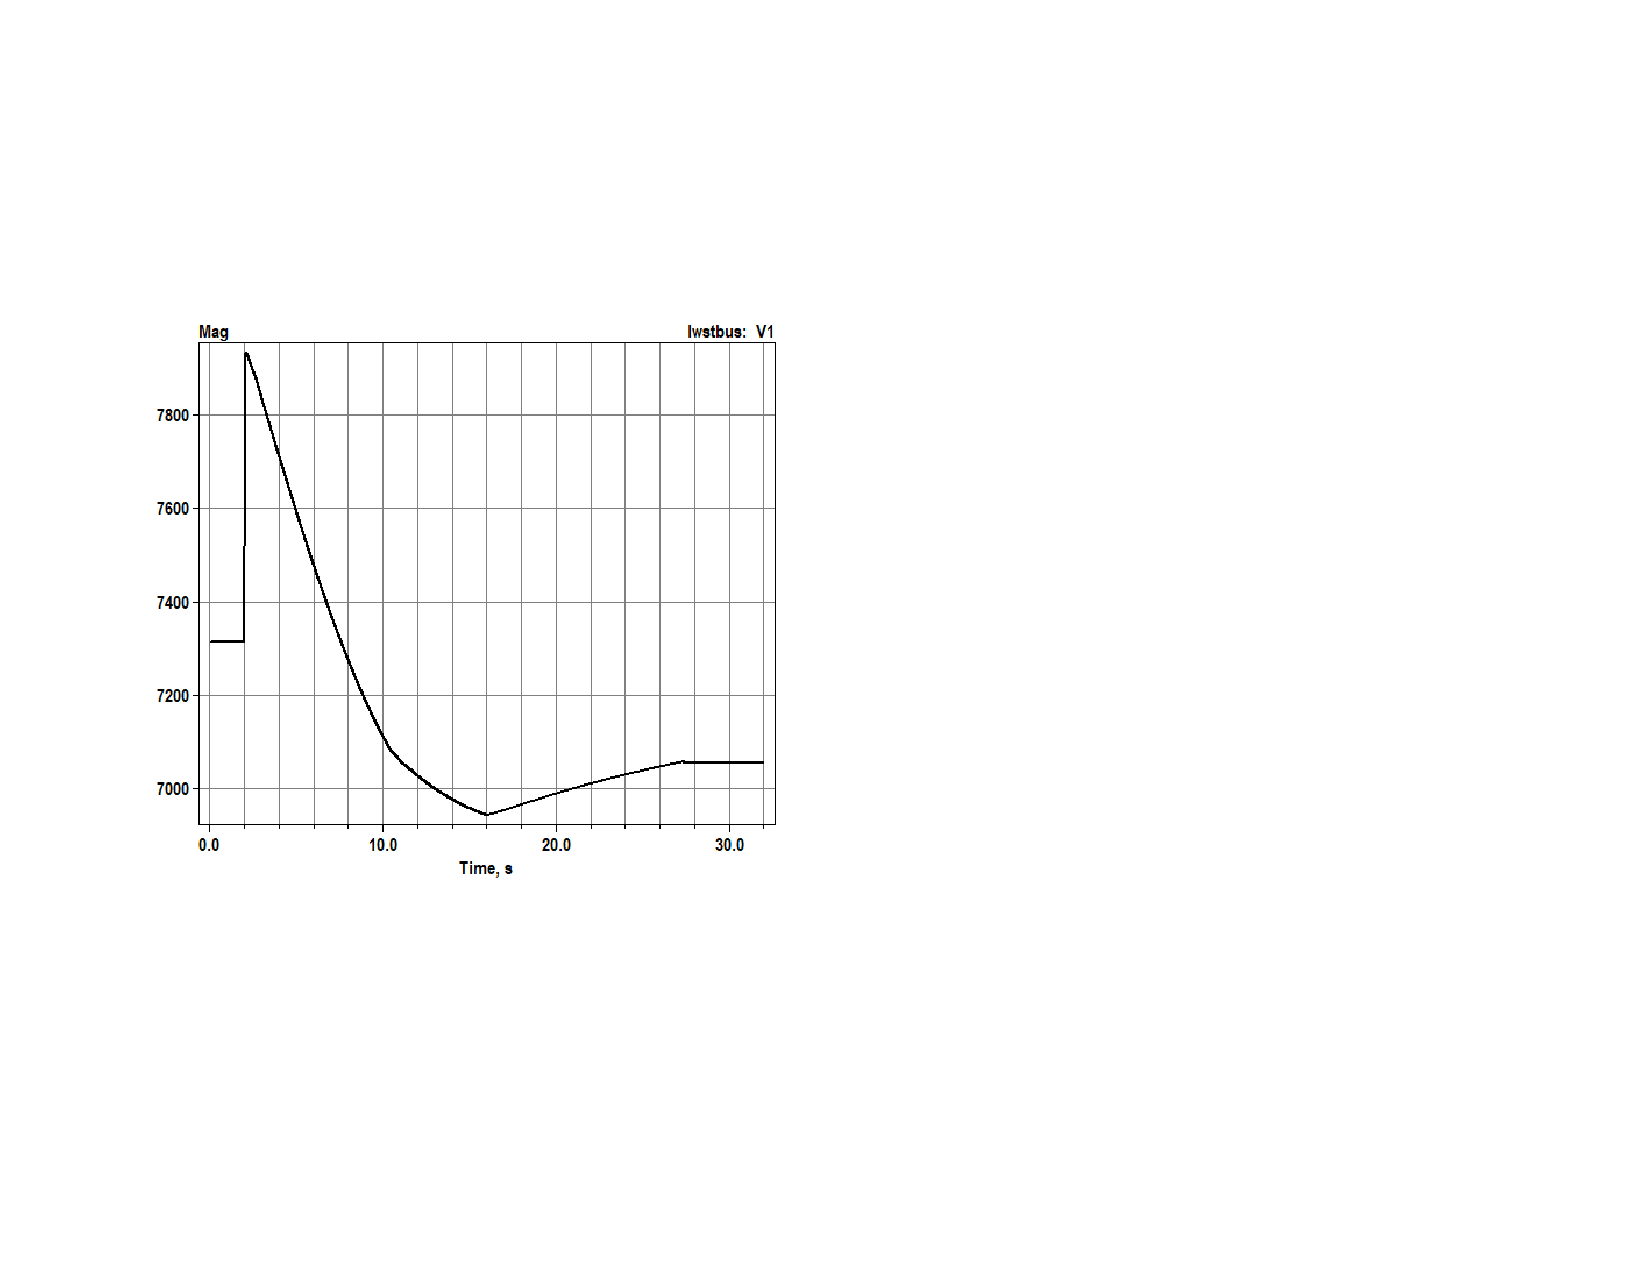
\includegraphics[height=5cm,width=0.45\linewidth]{pics/pqctrl1.pdf}
    }
    \subfloat[Bus voltage of DG1]{
    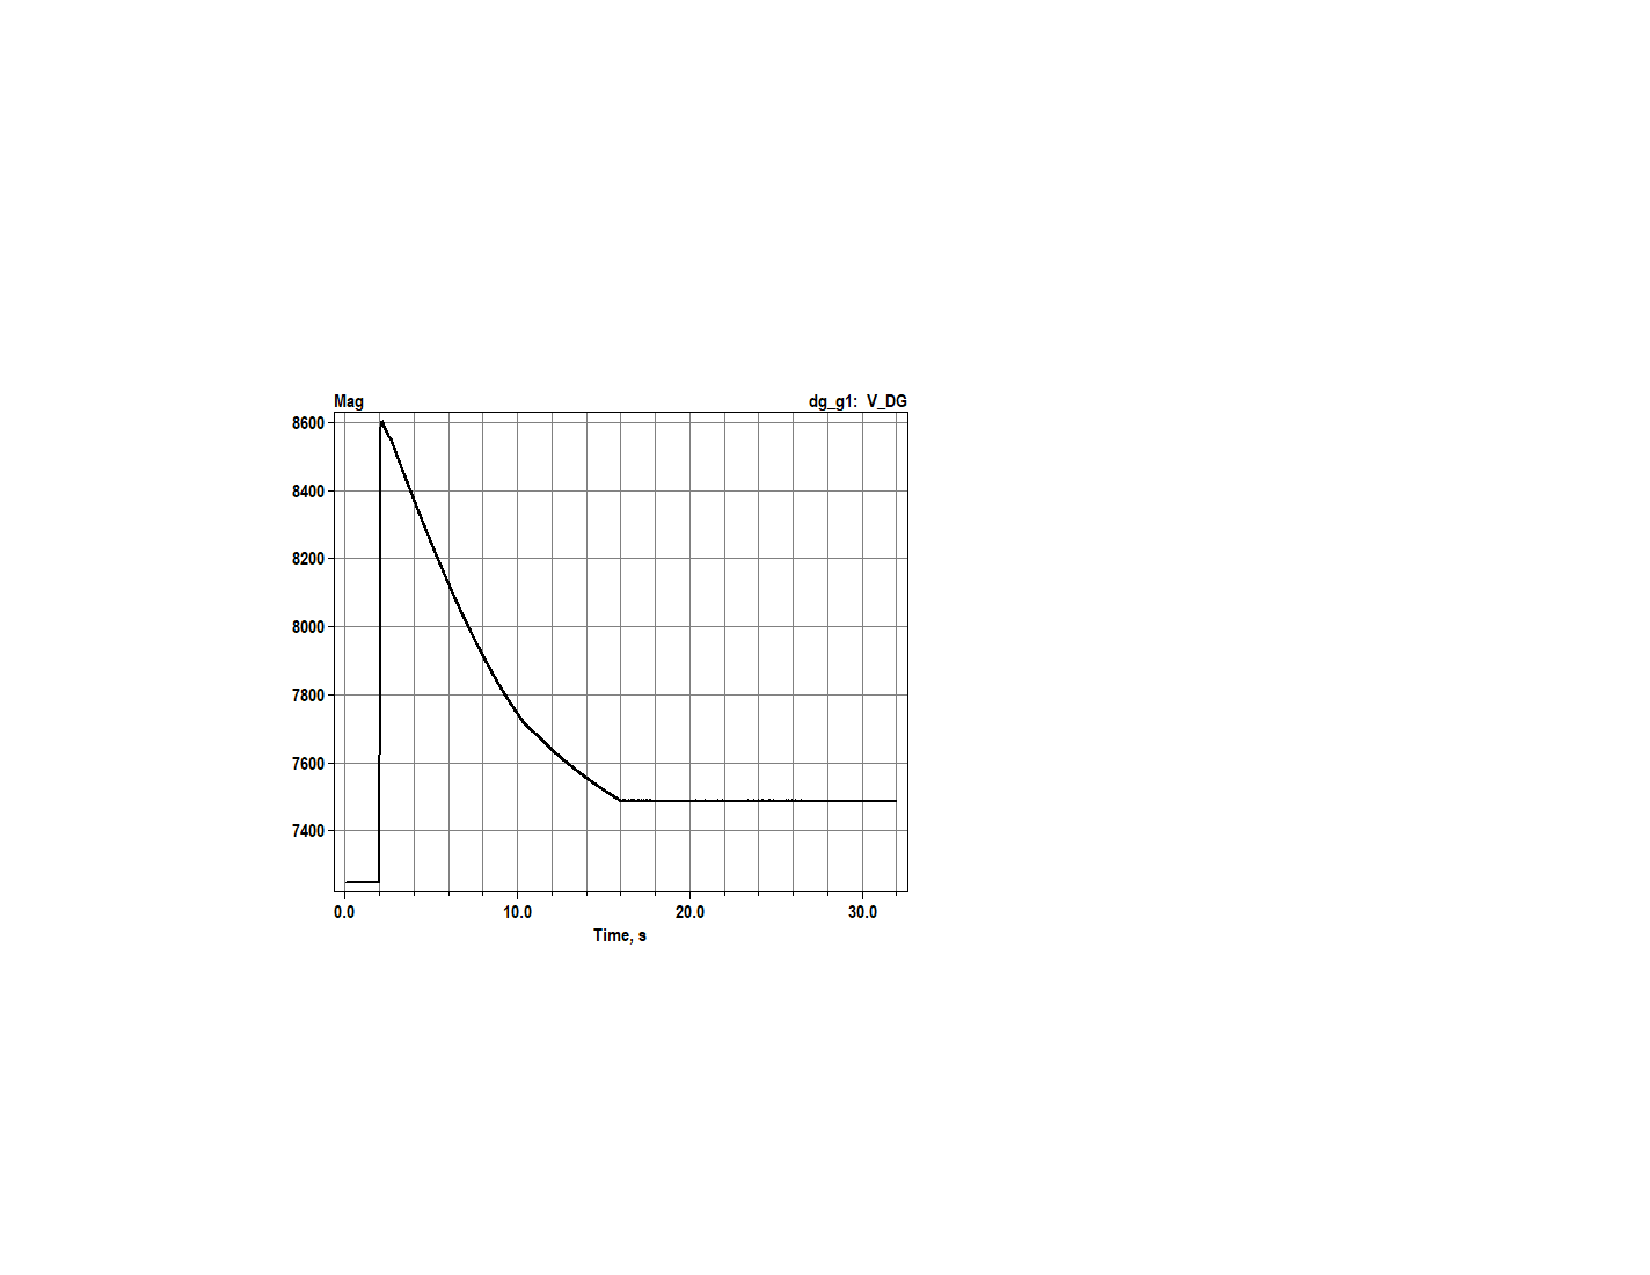
\includegraphics[height=5cm,width=0.45\linewidth]{pics/pqctrl2.pdf}
    }
    \quad
     \subfloat[Real power utilization ratio of DG1]{
    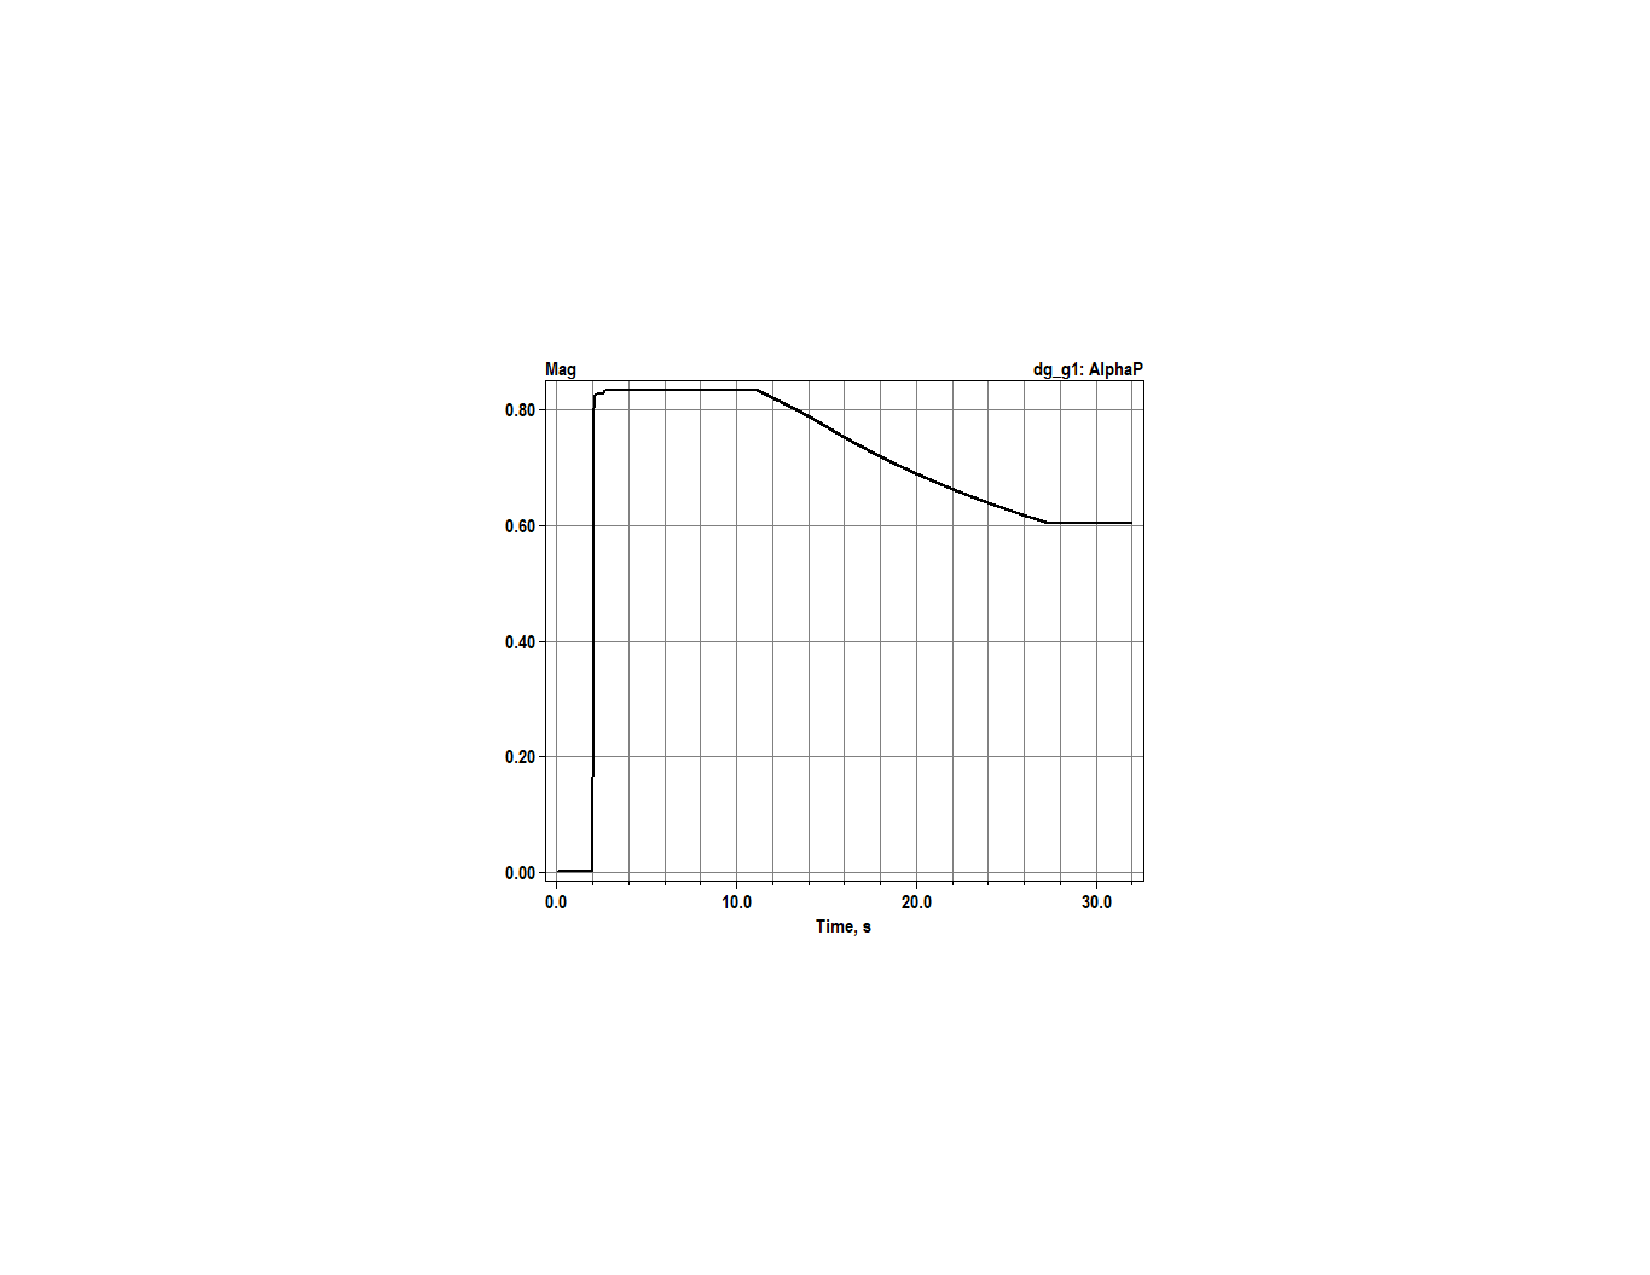
\includegraphics[height=5cm,width=0.45\linewidth]{pics/pqctrl3.pdf}
    }
    \subfloat[Reactive power utilization ratio of DG1]{
    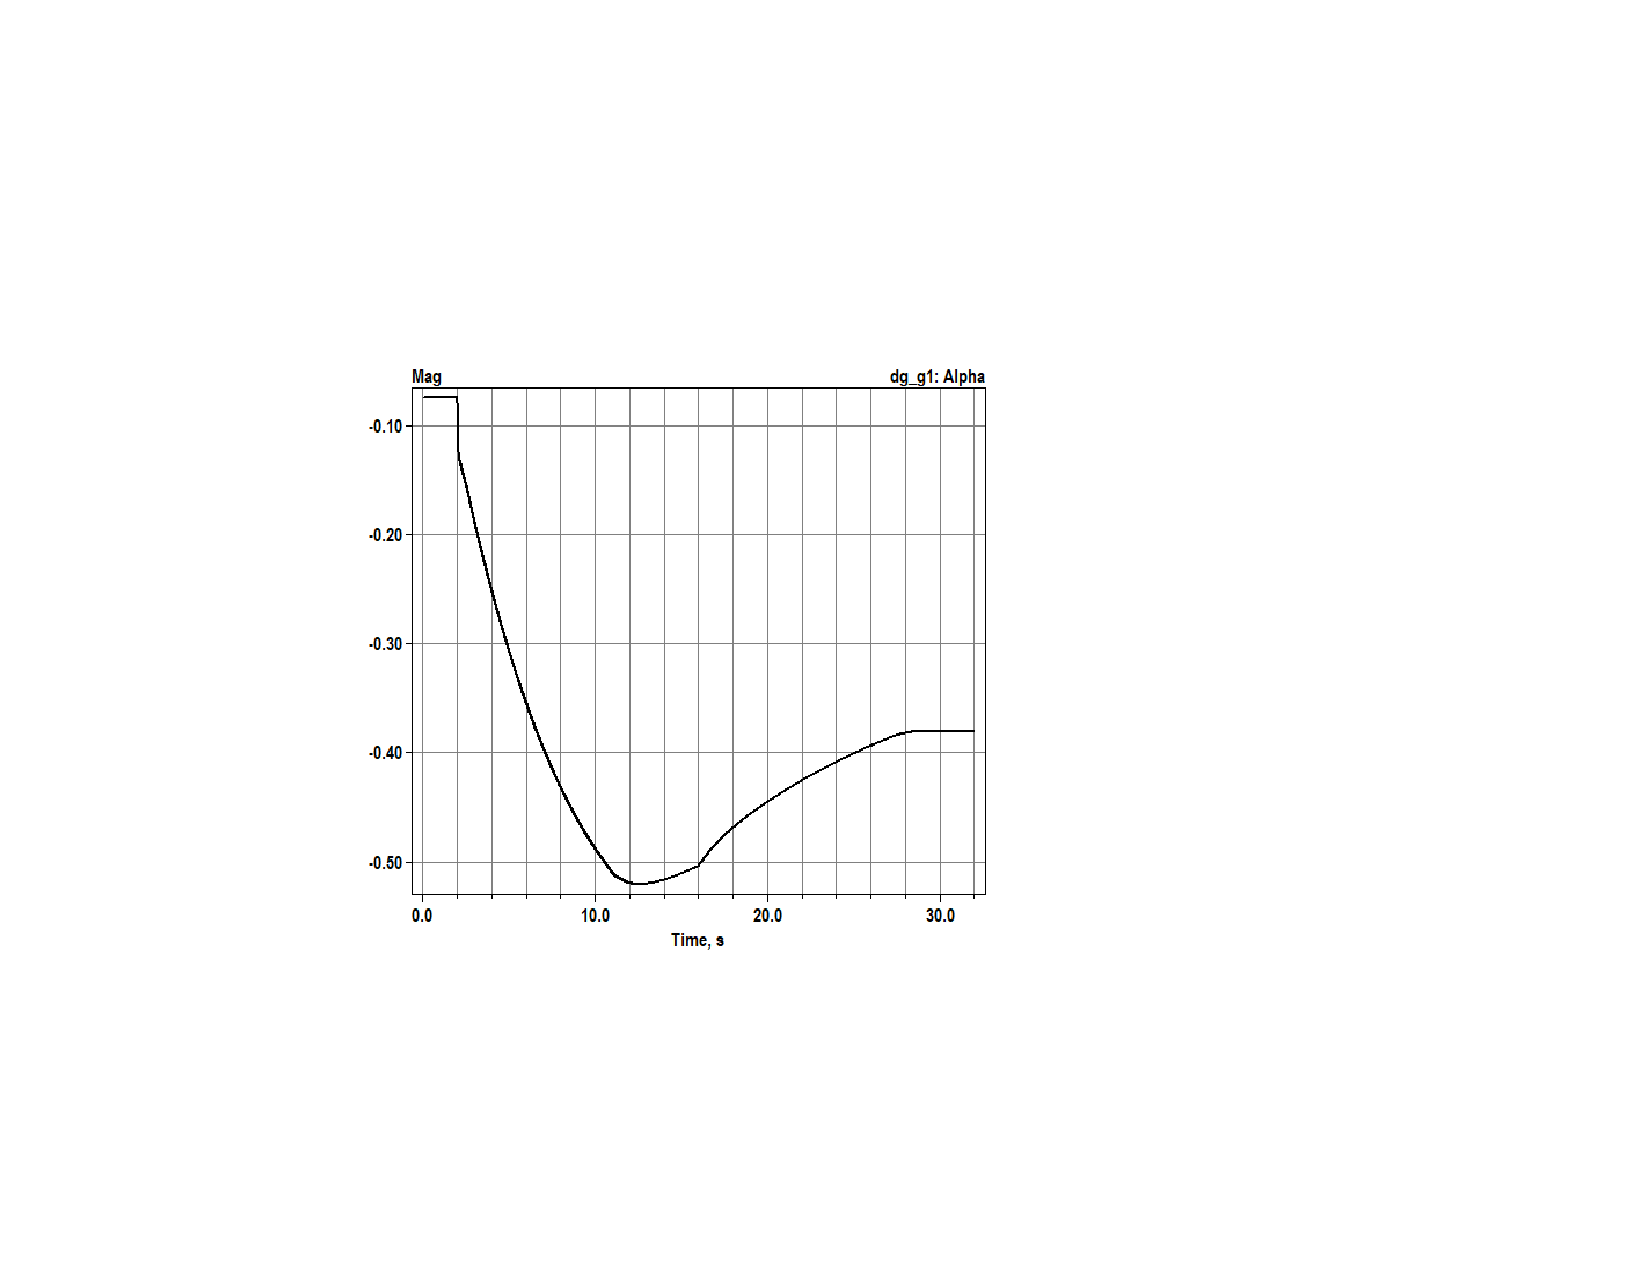
\includegraphics[height=5cm,width=0.45\linewidth]{pics/pqctrl4.pdf}
    }
    \caption{The control response of DGs to disturbance in the system}
    \label{fig:phctrl}
\end{figure}

\section{Islanded microgrid with high-penetration of DGs}
In the above control design, all inverters can be operated in PQ-mode (the grid-following control), because there are voltage and frequency references when the distribution network is connected to the main power grid through mid-voltage (MV) network. However in islanded mode, the reference for frequency and voltage control will not be available. In some design, a voltage and frequency (VF)-mode voltage source inverter (VSI) \cite{Lopes2006} is used to provide the reference for voltage and frequency as shown in Figure \ref{fig:frq_sg}, thus it is possible to operate the MG in islanded mode. 
\begin{figure}[ht]
    \centering
    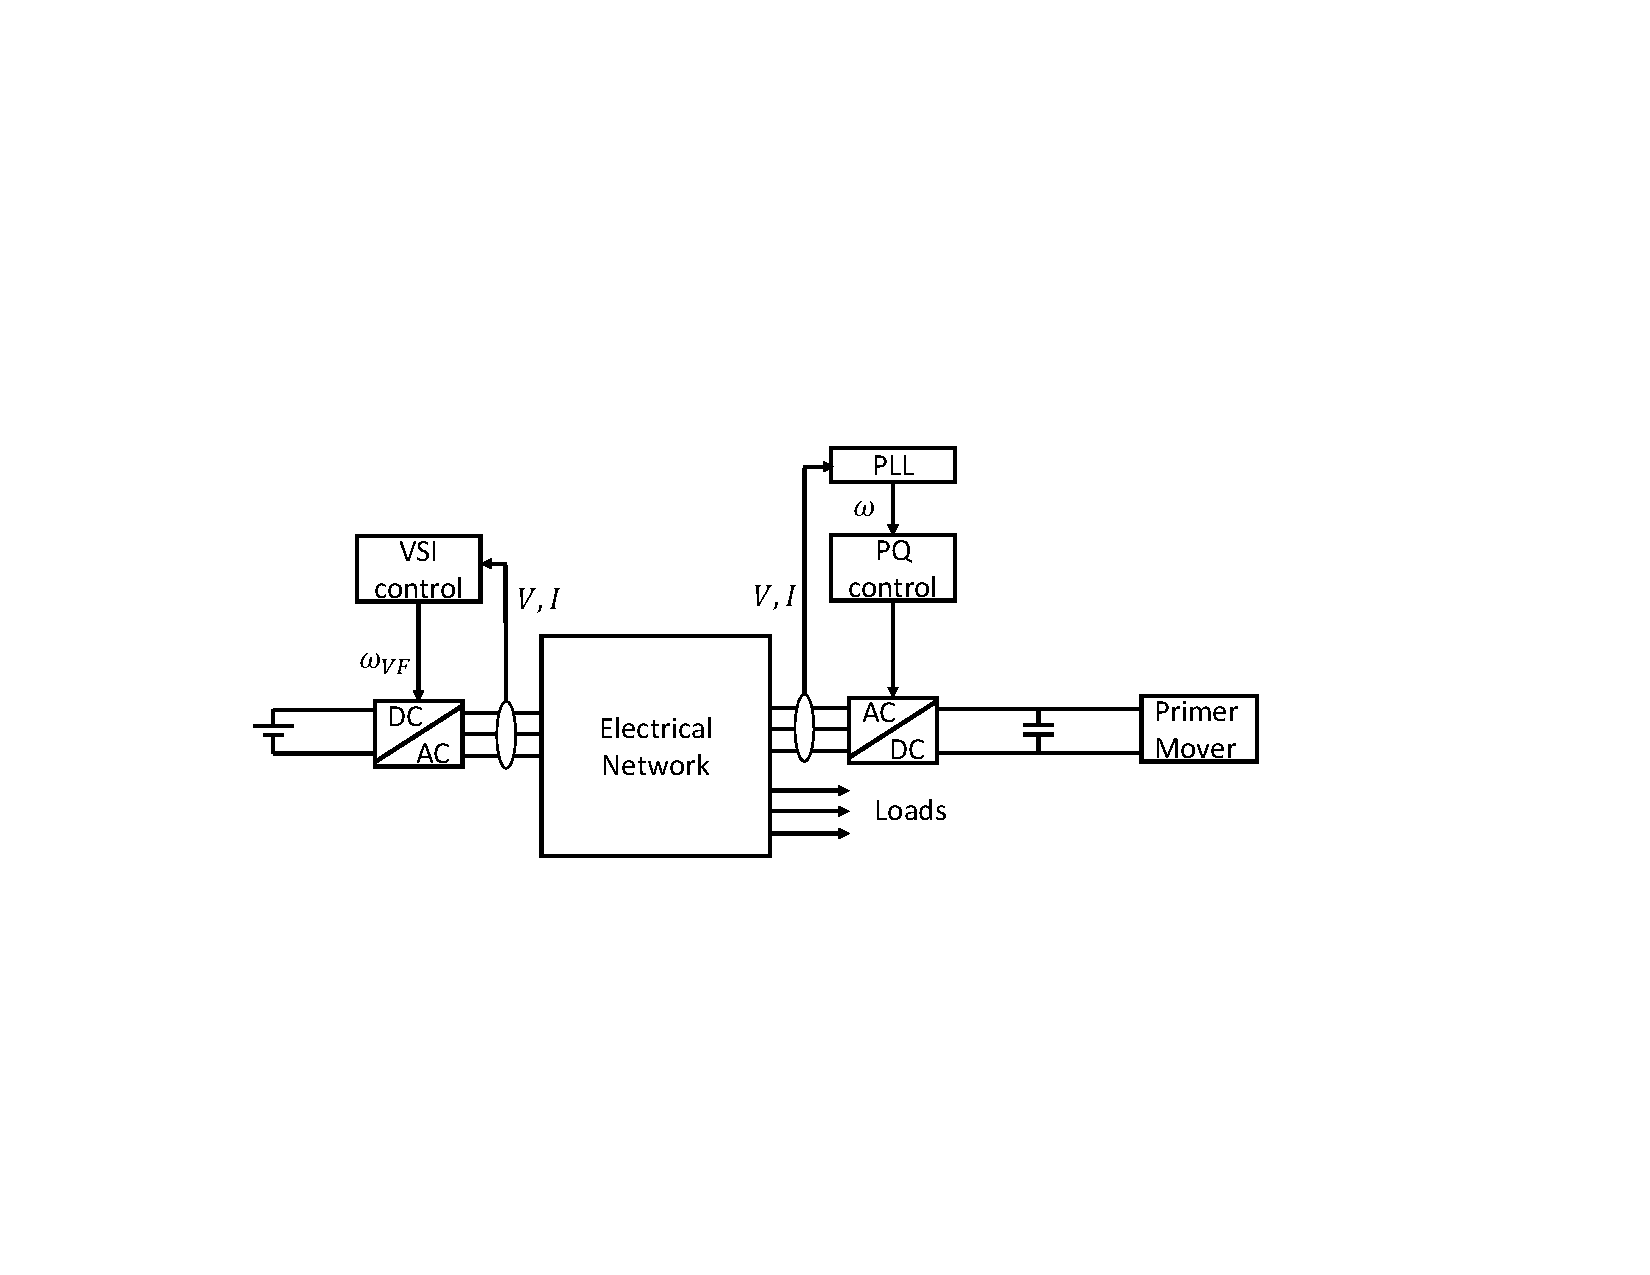
\includegraphics[width=\linewidth]{pics/vfmode.pdf}
    \caption{The reference for the islanded system operation}
    \label{fig:frq_sg}
\end{figure}

In islanded mode of microgrids, the output power of VF inverter (e.g. the energy storage systems) will balance out the load changes. The VF-mode inverter control deisgn can be categorized into three types \cite{Kroposki2017achieve}: (1) droop control, (2) virtual synchronous machine (VSM) and (3) nonlinear oscillator synchronization. Take VSM method for example, the bus angle, $\delta_{ref}$, and frequency, $\omega_{ref}$, can be modeled by the following strategy:
\begin{equation}
\left\{\begin{split}
    &\dot \delta_{ref} = \omega_{VF} - \omega_0\\
     &M \dot \omega_{VF} =  P_{VF}- P_{VF0}+D(\omega_{VF} - \omega_0)
\end{split} \right., \label{eq:drpi}
\end{equation}
where $\omega_0$ is the nomimal value of frequency, $P_{VF}$ and $P_{0}$ are the instantaneous and nominal power of VF-mode ESS respectively, $M$ and $D$ are coefficiencies of VSM design.

The PQ-mode DGs are assumed to follow the control command. In this scenario, let's assume the droop ratio $m_i$ for each of the PQ inverters,
then the power desired in the system (which is the output power of the VF inverters) can be distributed among all PQ inverters by the following droop strategy (as shown in Figure \ref{fig:fdroop}):
\begin{equation}
    P_{VF}- P_{VF0} =  \sum m_i(\omega_0-\omega_i), \label{eq:drpi}
\end{equation}
where $\omega_i$ is the instantaneous frequency measured by PLL (phasor lock loop) at the connection bus, which is generated by VF inverters ($\omega_{VF}$) and spread though the electrical network. Hence we have
\begin{equation}
    \omega_i = \omega_{VF},
\end{equation}
given the dynamic of PLL is neglected.
\begin{figure}[ht]
    \centering
    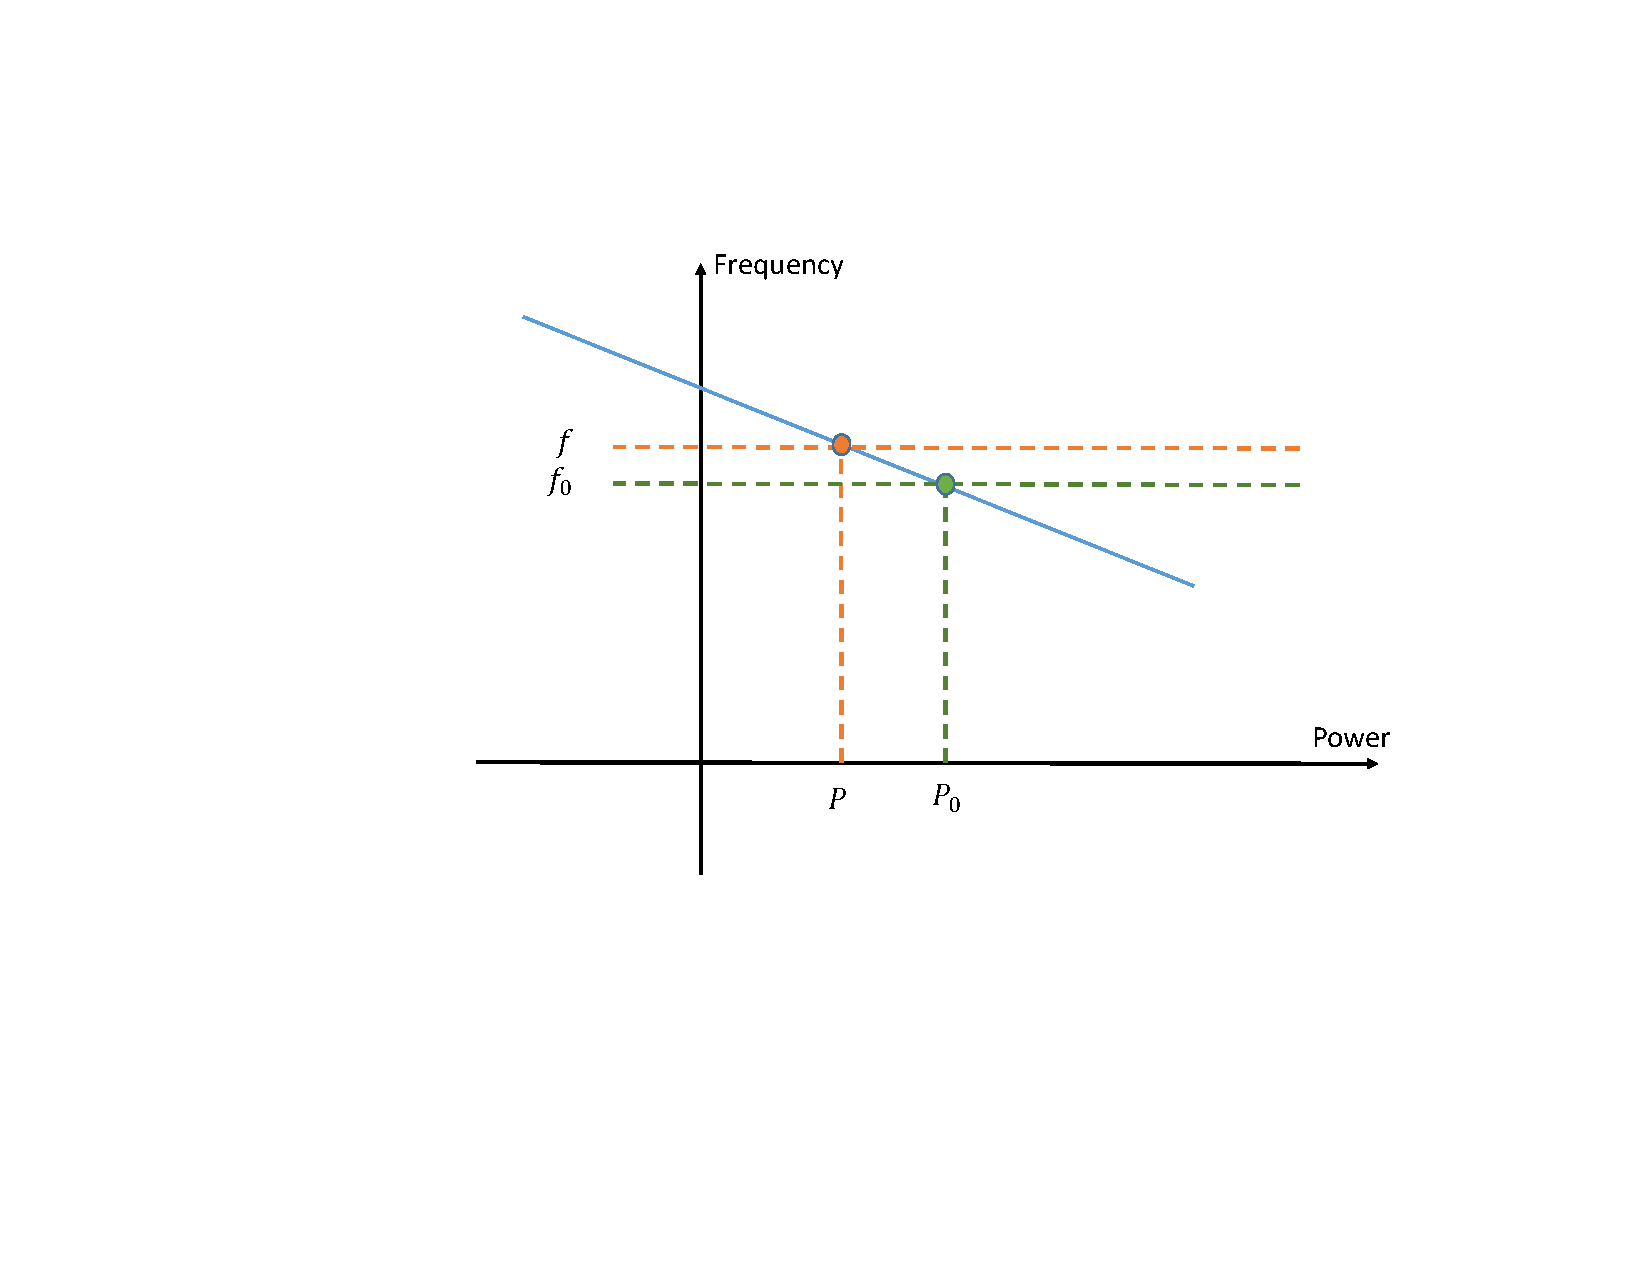
\includegraphics[width=\linewidth]{pics/fdroop.pdf}
    \caption{The droop strategy for PQ inverters}
\label{fig:fdroop}
\end{figure}

It is clear that the VF inverters in the islanded mode work the same as the slack bus. So in the islanded mode, we can split all VF inverters as the slack bus and apply the same control strategy \eqref{eq:cclz} to the rest DGs.  
The power dispatch in \eqref{eq:fif} is equivalent to the output of VF inverters, i.e.
\begin{equation}
    P^*_{f}- P_f = P_{VF}- P_{VF0},
\end{equation}
then we have, 
\begin{equation}
    P^*_{f}- P_f = \sum m_i(\omega_0-\omega_{VF}).
\end{equation}
Hence, similar to \eqref{eq:fif}, the control objective for the real power control in islanded mode can be written as follows 
\begin{equation}
    f_i =\frac{\lambda^{f}_i}{2}(\omega_0-\omega_{VF})^2+
    \frac{\lambda^{v}_i}{2}(V_{i}^{*}-V_{i})^2+\frac{\lambda^p_i}{2}(P^{ref}_{g_i}-P_{g_i})^2 \label{eq:fisld}
\end{equation}
where $\lambda_i^{f}\geq 0$, $\lambda^{v}_i\geq 0$ and $\lambda^{p}_i\geq 0$ are the coordinate coefficients at the $i^{th}$ agent; $P_{g_i}$ stands for the power injection of the $i^{th}$ agent; $V_{i}$ is the representative voltage of the $i^{th}$ agent, particularly, the worst measured voltage at that agent. We use $\lambda^{f}_i$ to include the information of the droop gains ($m_i$s) for the simplicity of expression.

The distributed subgradient algorithm \eqref{eq:ccl} is used again to control the real power in order to pursue the above goal. The subgradient of objective function defined by \eqref{eq:fisld} can be calculated in the same way as in section \ref{sec:syslvl}: the subgradients of $\frac{\lambda^{v}_i}{2}(V_{i}^{*}-V_{i})^2$ and $\frac{\lambda^p_i}{2}(P^{ref}_{g_i}-P_{g_i})^2$ are the same as in \eqref{eq:gik}. The derivative of $\frac{\lambda^{f}_i}{2}(\omega_0-\omega_{VF})^2$ with respect to $P_{g_k}$ can be calculated as follows:
\begin{equation}
    \frac{\partial \frac{\lambda^{f}_i}{2}(\omega_0-\omega_{VF})^2 }{ \partial P_{g_k}} =\lambda^{f}_i m_k (\omega_0-\omega_{VF}).\label{eq:domg}
\end{equation}

Using \eqref{eq:domg} and \eqref{eq:dvpl}, the subgradient of \eqref{eq:fisld} can be obtained and hence the real power control for islanded mode is complete. It is necessary to emphasize in the islanded mode the frequency and power balance is of much more importance than other objectives. This will be
reflected in the design of coordinate coefficients, and an extreme case is to set $\lambda^{v}_i$ and $\lambda^{p}_i$ to zero and the objective becomes
\begin{equation}
    f_i =\frac{1}{2}(\omega_0-\omega_{i})^2.   
\end{equation}
In this case, the algorithm regress to droop control. The fair utilization ratio method \eqref{eq:dalfap} is also applicable:
\begin{equation}
    \dot \alpha_{p_i} = \sum_{j \in N_i^c}d_{ij} (\alpha_{p_j}-\alpha_{p_i}) - \beta_i g^p_{i},  \label{eq:dalfapf}
\end{equation}
where $g^p_{i}$ is the subgradient of $f_i$ which can be calculated from the above procedure. For reactive power control in the islanded microgrid, the same control \eqref{eq:dalfaq} is applied according to the above local voltage control strategy (principal \ref{principal}).

Using OpenDSS, we evaluate the performance of the above control scheme by standard IEEE system: 8500-node circuit. A virtual synchronous generator model is used to generate the frequency reference in the system, as shown in Figure \ref{fig:vsm}. The stiff source bus is simulated by the classic synchronous machine model with the constant inner bus voltage behind transient admittance of the generator. Then the frequency of islanded system can be generated by the frequency of the VSM.
\begin{figure}[ht]
    \centering
    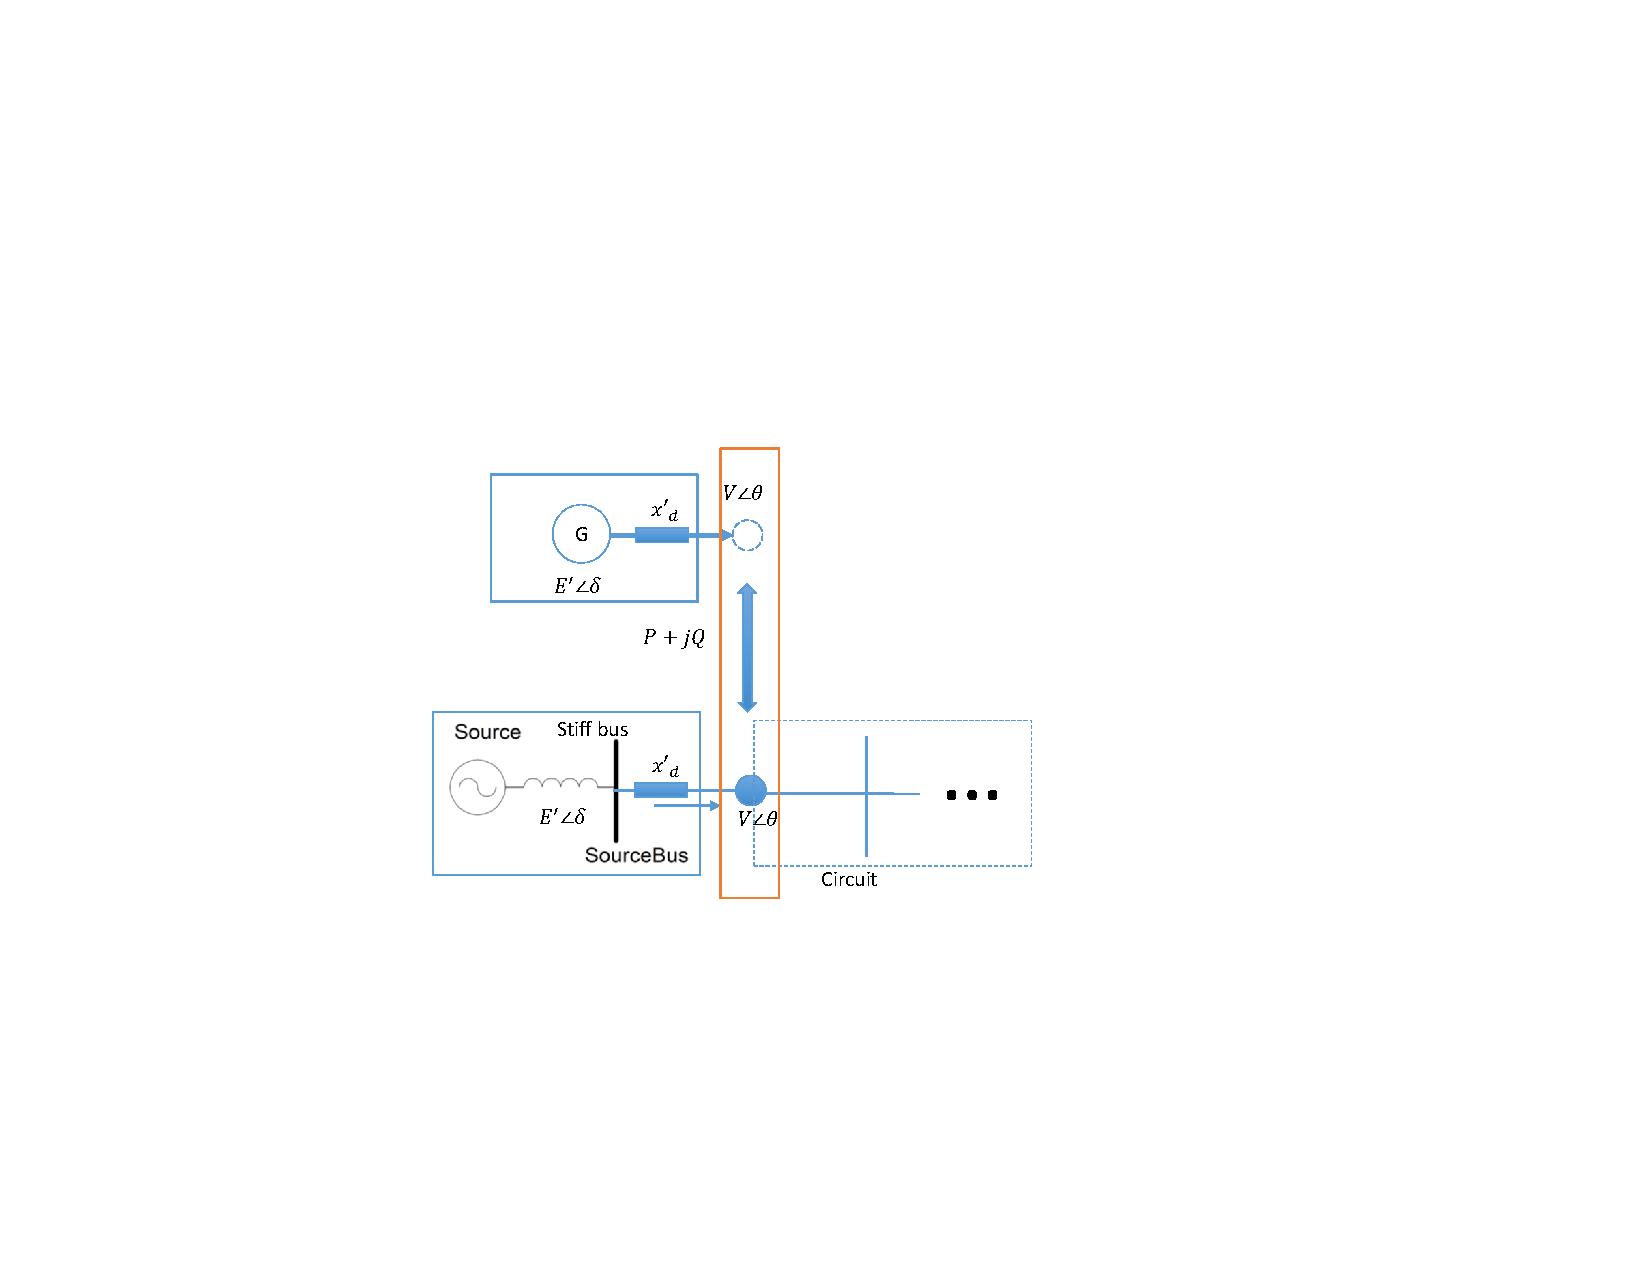
\includegraphics[width=0.9\linewidth]{pics/vsm.pdf}
    \caption{The stiff source bus is simulated as the inner bus behind transient admittance of a virtual synchronous generator}
    \label{fig:vsm}
\end{figure}
A worst scenario found by the greedy search method \cite{rathbun2018impact} of the system with 4 large-scale PV farms and 100\% penetration is shown in Figure \ref{fig:f8500}. 
\begin{figure}[h!]
    \centering
    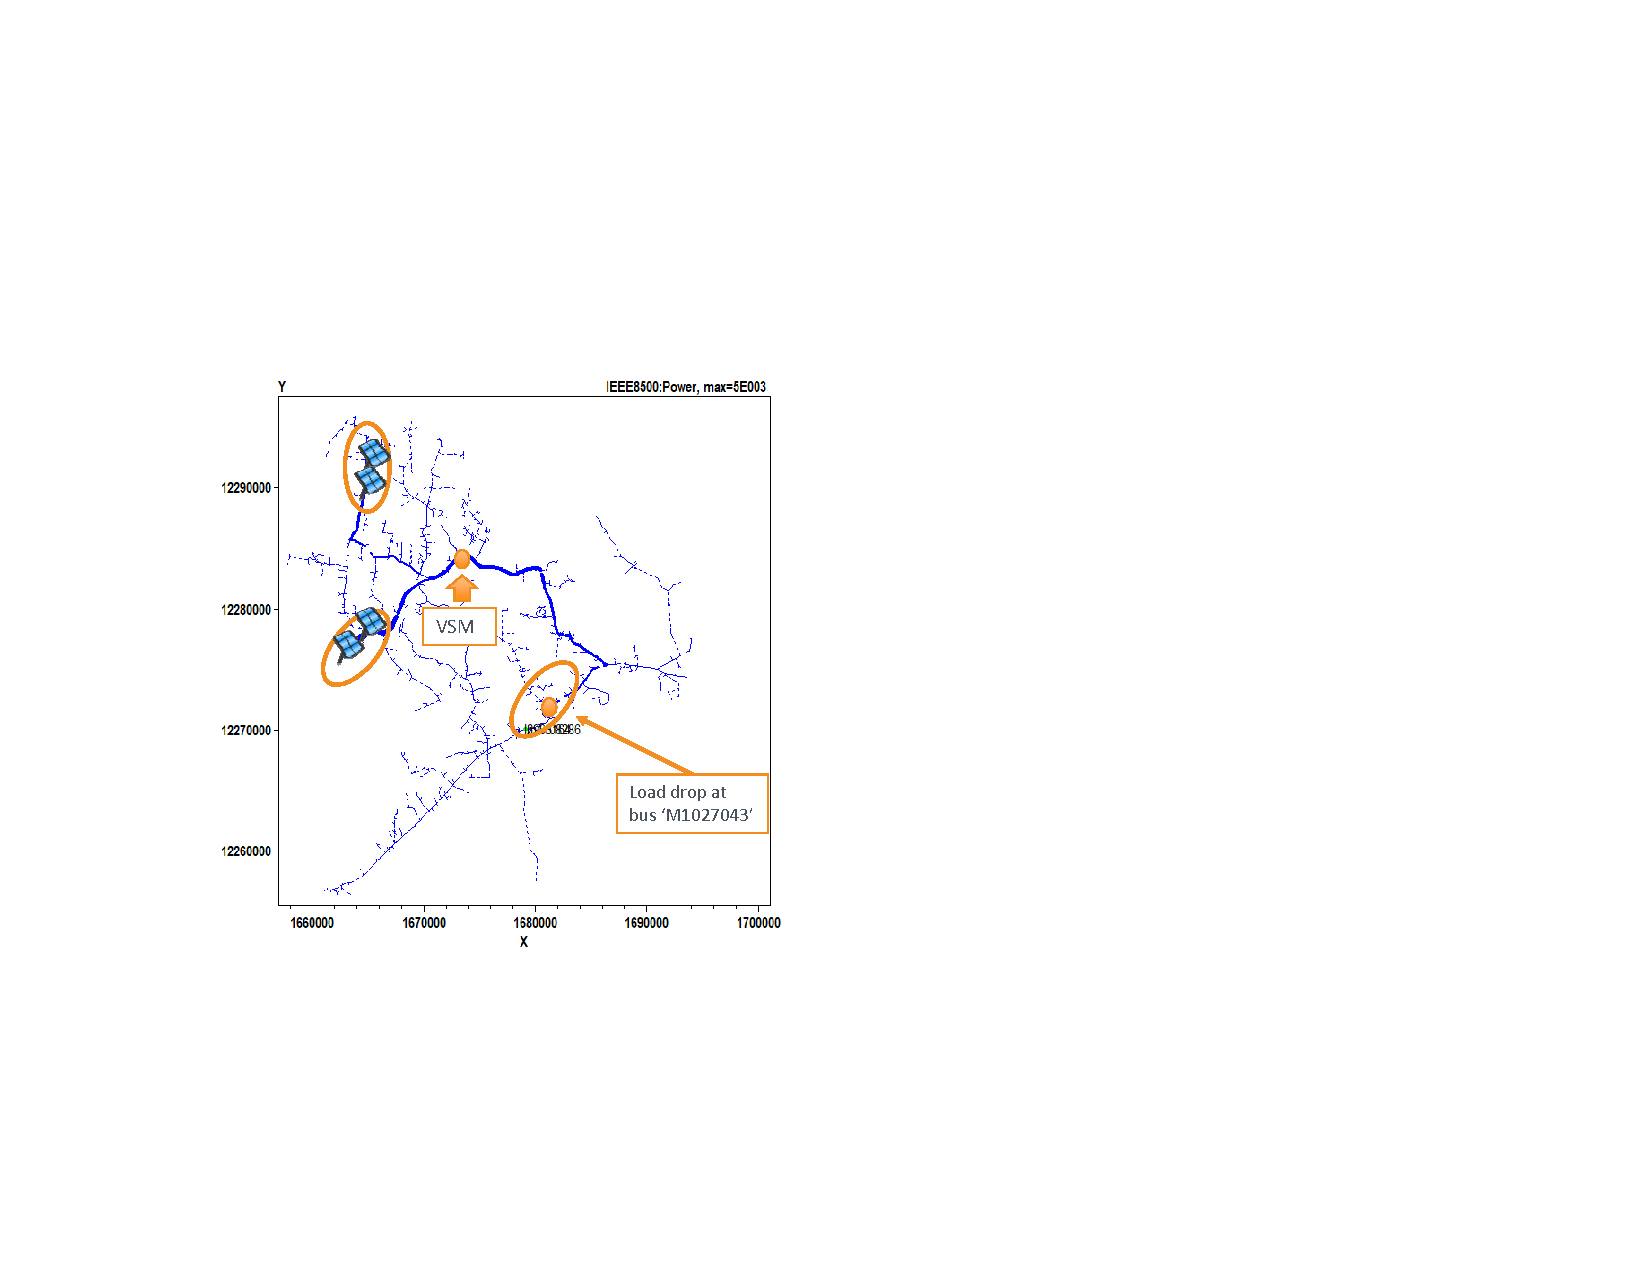
\includegraphics[width=\linewidth]{pics/f8500.pdf}
    \caption{The worst scenario of IEEE 8500 system with 4 large-scale PVs}
    \label{fig:f8500}
\end{figure}

First, we built up an islanded system by opening the breaker at the feeder of IEEE 8500-node circuit, and using VSM to supply $300kW$ at connection bus, assuming the reactive power supply is sufficient to maintain the inner bus voltage. Secondly, all regulators of the circuit are fixed at the predefined positions during the control. 
To test the active power and frequency control, we use dynamic simulation mode in OpenDSS. The simulation is set as simulation time $T=30s$ with time step $h=0.005s$. A system disturbance of $2MW$ load drop happens at $t_0=0.7s$. As shown in Figure \ref{fig:frslts}, the proposed algorithm is effective for system frequency control in case of islanded operation of distribution system. When the demand of one load decreases at $0.7s$, the system frequency starts to increase correspondingly. Then the active power control of PVs respond to the change of frequency. As a result, both the frequency is well maintained by the proposed control. At the same time, the reactive power control is also effective to maintain the system voltages.
\begin{figure}[ht]
    \centering
    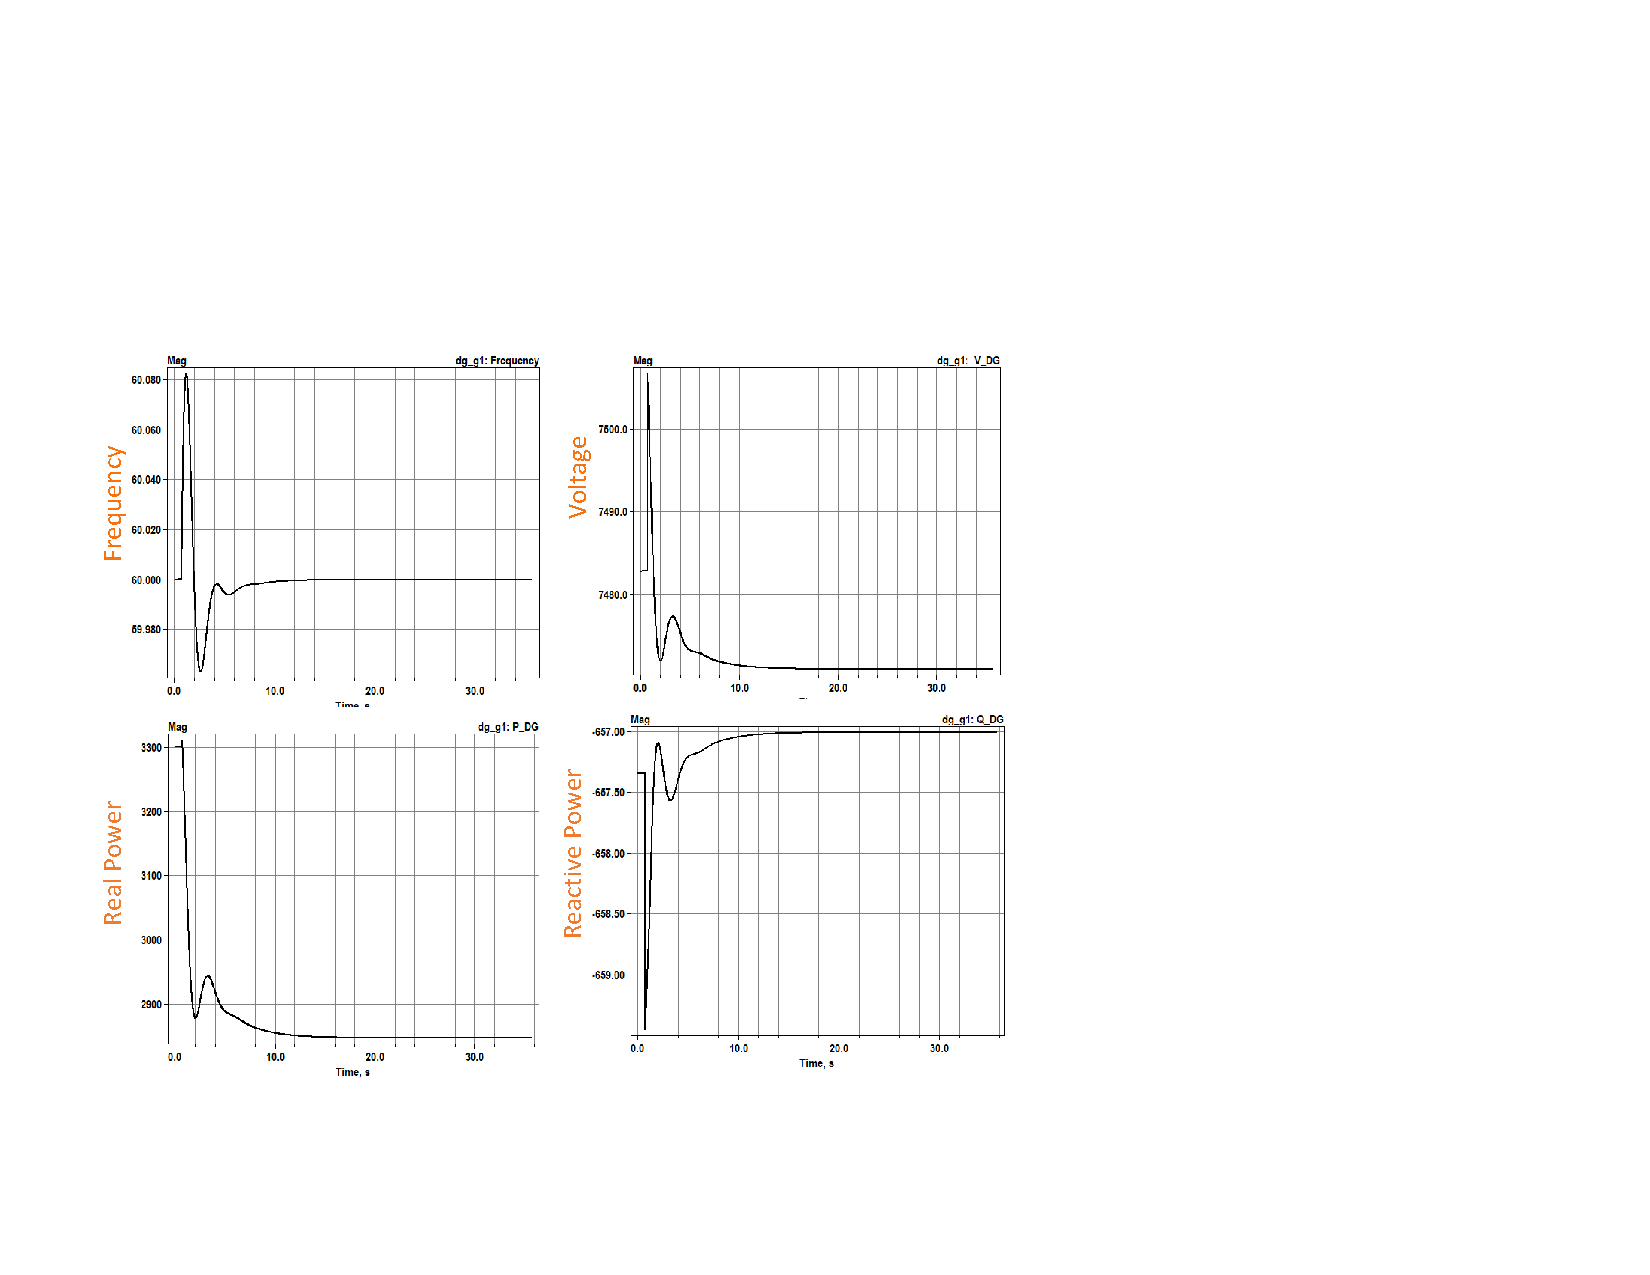
\includegraphics[width=\linewidth]{pics/frslts.pdf}
    \caption{The frequency control of IEEE 8500-node system on islanded mode }
    \label{fig:frslts}
\end{figure}

\section{Grid-edge situational awareness: enhanced observability by voltage inference}\label{sed:gridedge}
There are synchronous measurement and control units (SMUs) and asynchronous measurement units (AMUs) in distribution systems. While SMUs are probably limited, AMUs should be deployed on all the load buses. The insufficiency of SMUs is the reason of the low observability of distribution network. However, it is not difficult and less expensive to upgrade AMUs for a smaller time interval of information gathering. It is possible to infer the system situation using information from both SMUs and AMUs. To this end, we present a sensitivity-based grid-edge situational awareness method in this section.  
\subsection{Voltage inference method}
Assume some of the buses have SMUs,  while the rest buses do not. Instead, the rest buses have AMUs which can update their information for a particular period of time, $T$, which can be $5$ minutes or several hours.

We summarise two types of distribution network voltage inference scenarios in Figure \ref{fig:vgrdnt}. In this figure, there are prosumers under some of the buses $i$, $j$, $k$, $m$ and $n$. The net power injection (direction defined by arrow) of each prosumer is denoted by $P_*+jQ_*$, where the subscript $*$ represents the bus number. The blue block represents the real-time measurement and control unit while the yellow block denotes off-line measurement. The two scenarios of operational situation awareness for presumer-dominated distribution systems are (I) subtree type ( Figure \ref{fig:sub}), 
 %(ii) belly type (see Figure \ref{fig:bly}) 
 and (II) the two-end type (Figure \ref{fig:mix}). Type (I) represents a typical scenario in distribution network that, bus $i$ is a SMU, but in the subtree of bus $i$, all buses are AMUs; Type (II) is for a portion of circuit that the two ends are SMUs; and most of other cases can be considered as a kind of the mix of these two types. Hence in the following analysis, we will focus on the voltage inference of the two types of distribution network. 
\begin{figure}[t]
    \centering
    \subfloat[subtree type]{
    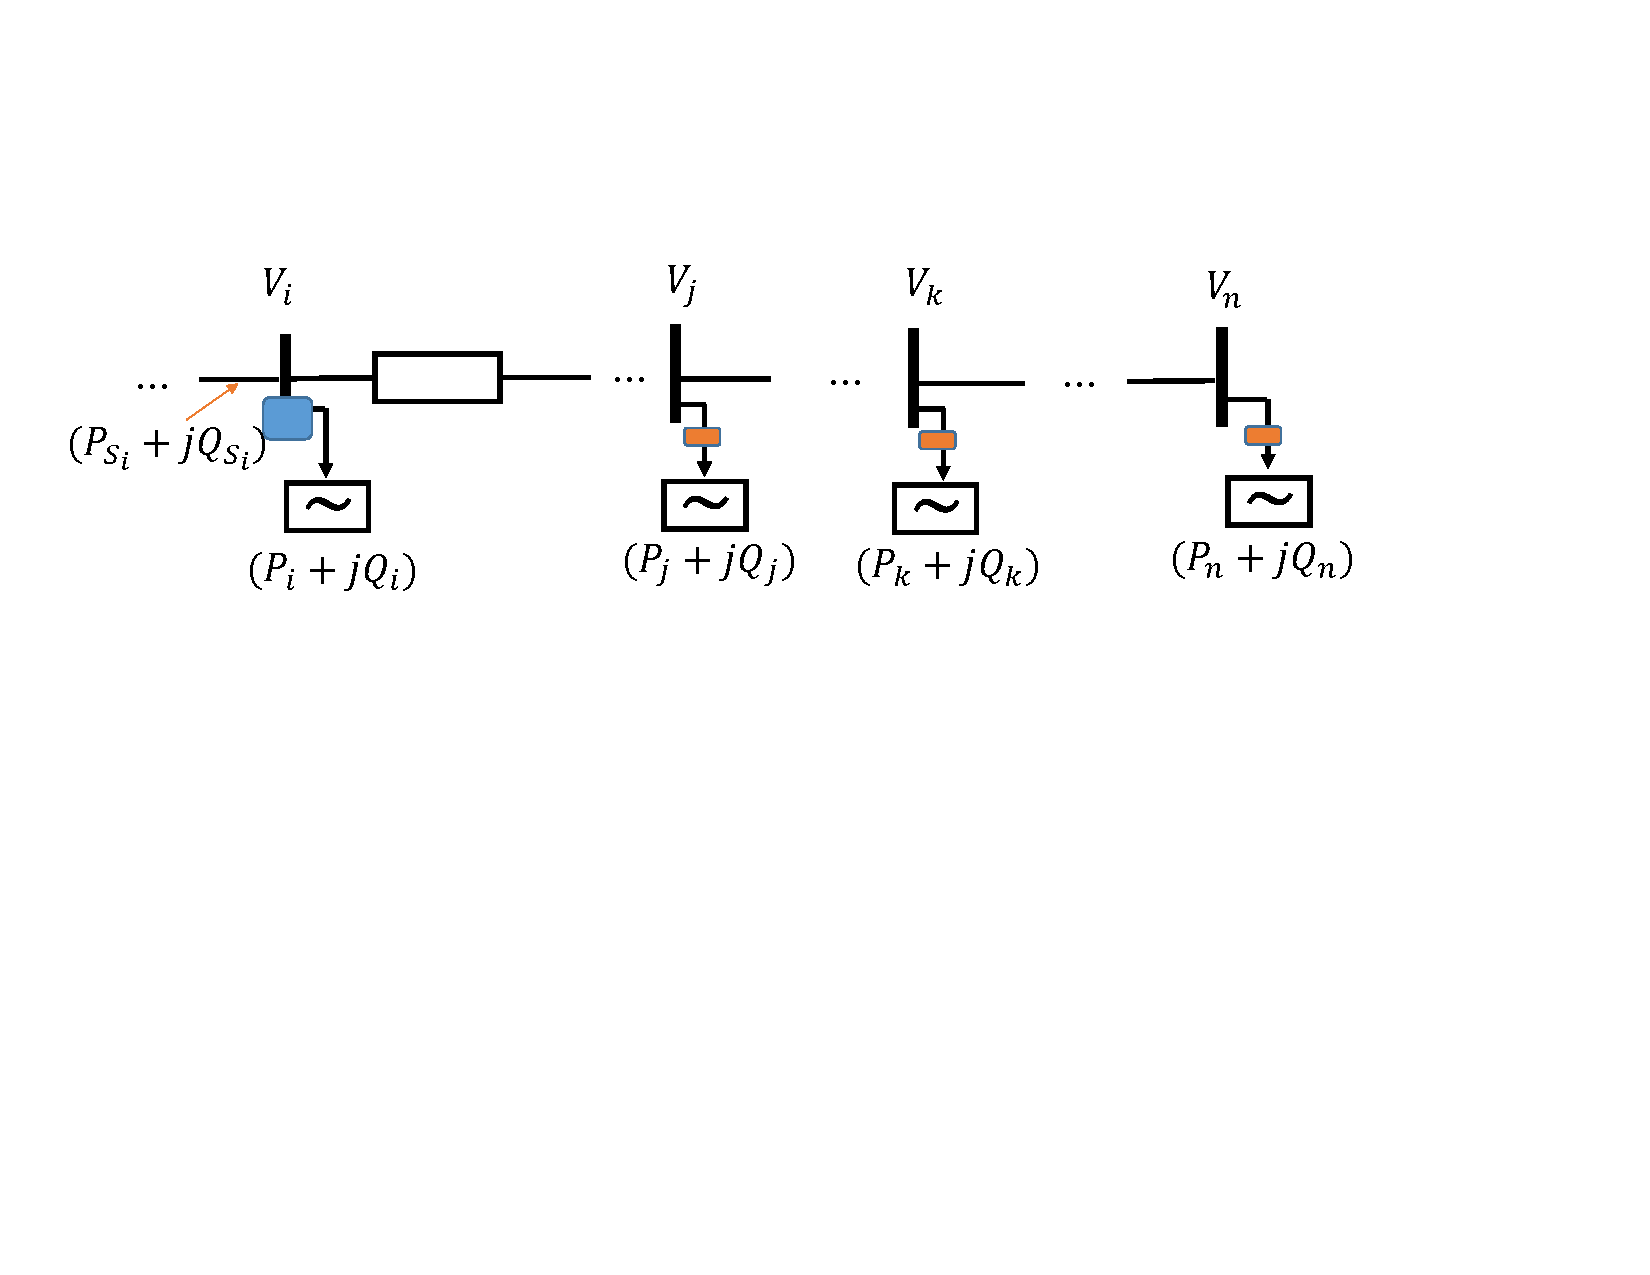
\includegraphics[width=\linewidth]{pics/vgrdnt1.pdf}
    \label{fig:sub}
    }
%    \quad
%    \subfloat[belly type]{
%    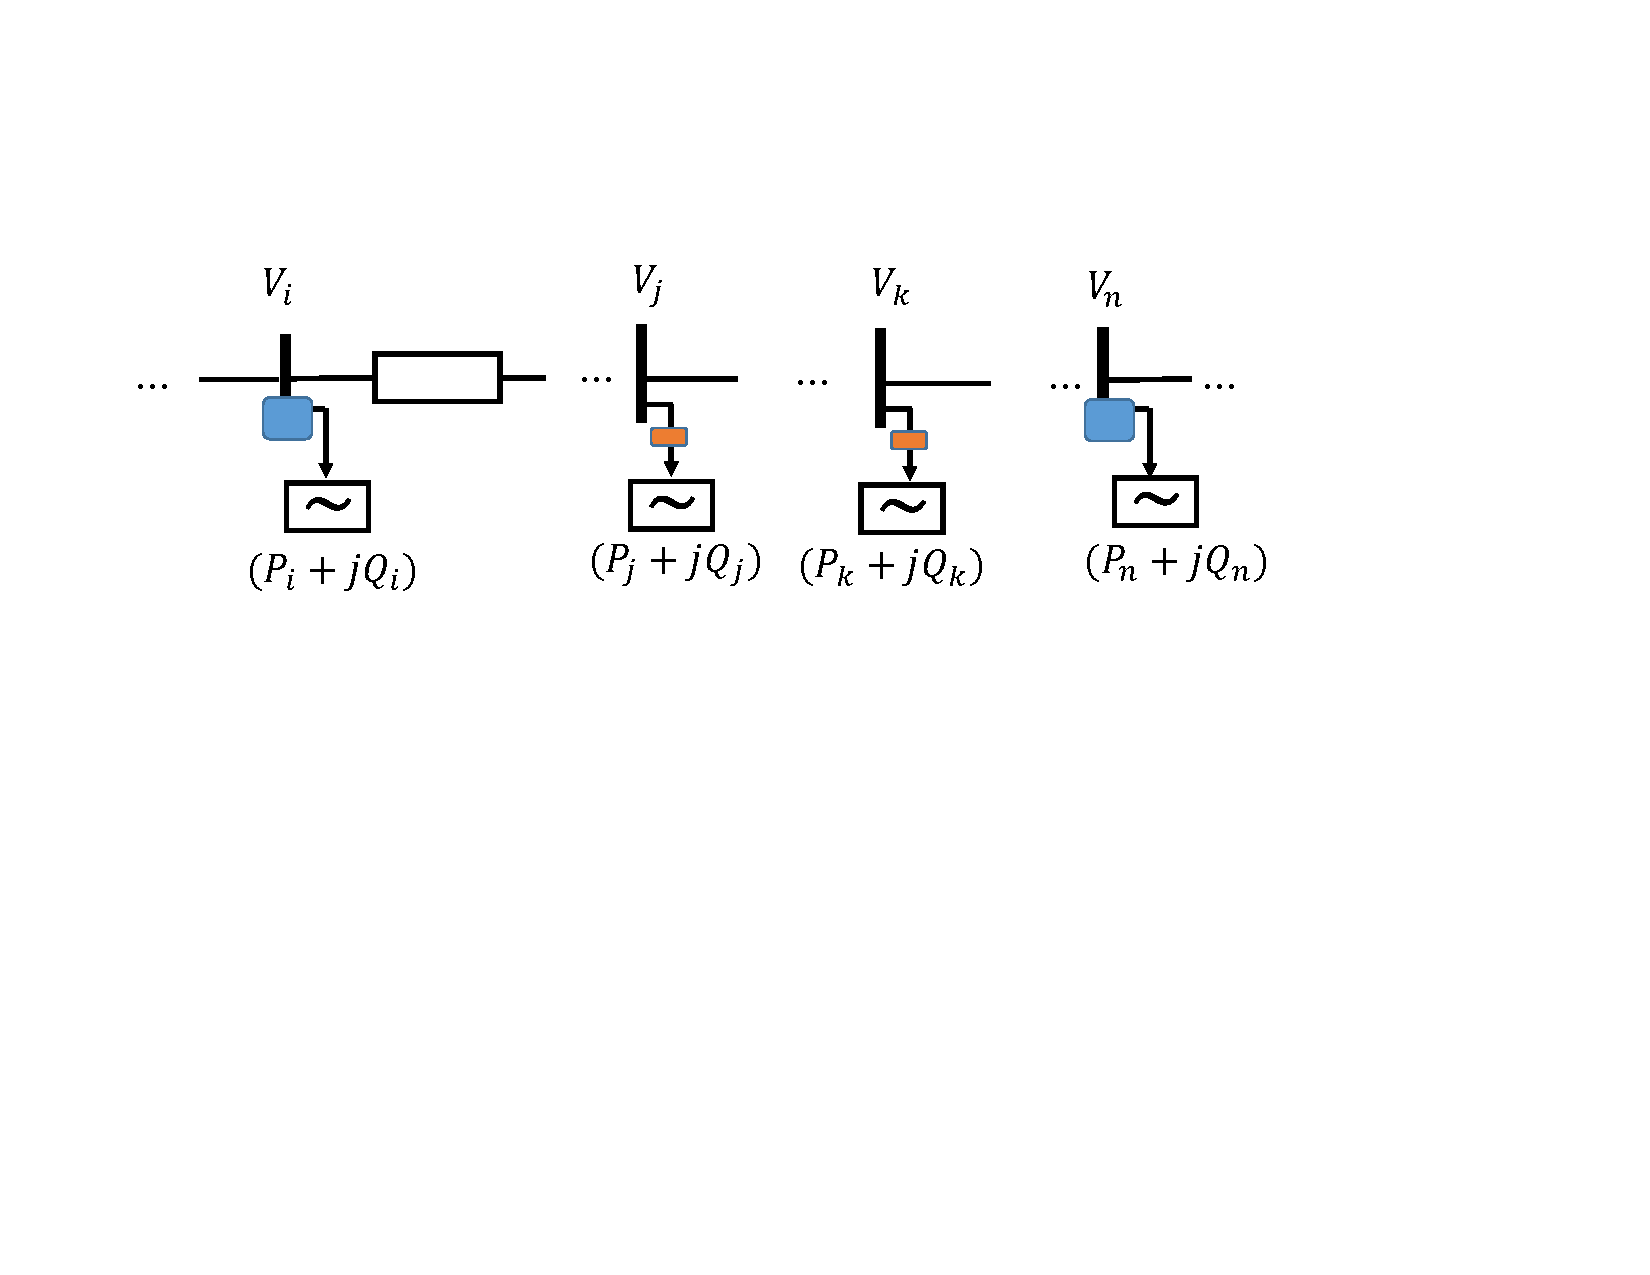
\includegraphics[width=\linewidth]{pics/vgrdnt2.pdf}
%    \label{fig:bly}
%    }
    \quad
    \subfloat[mix type]{
    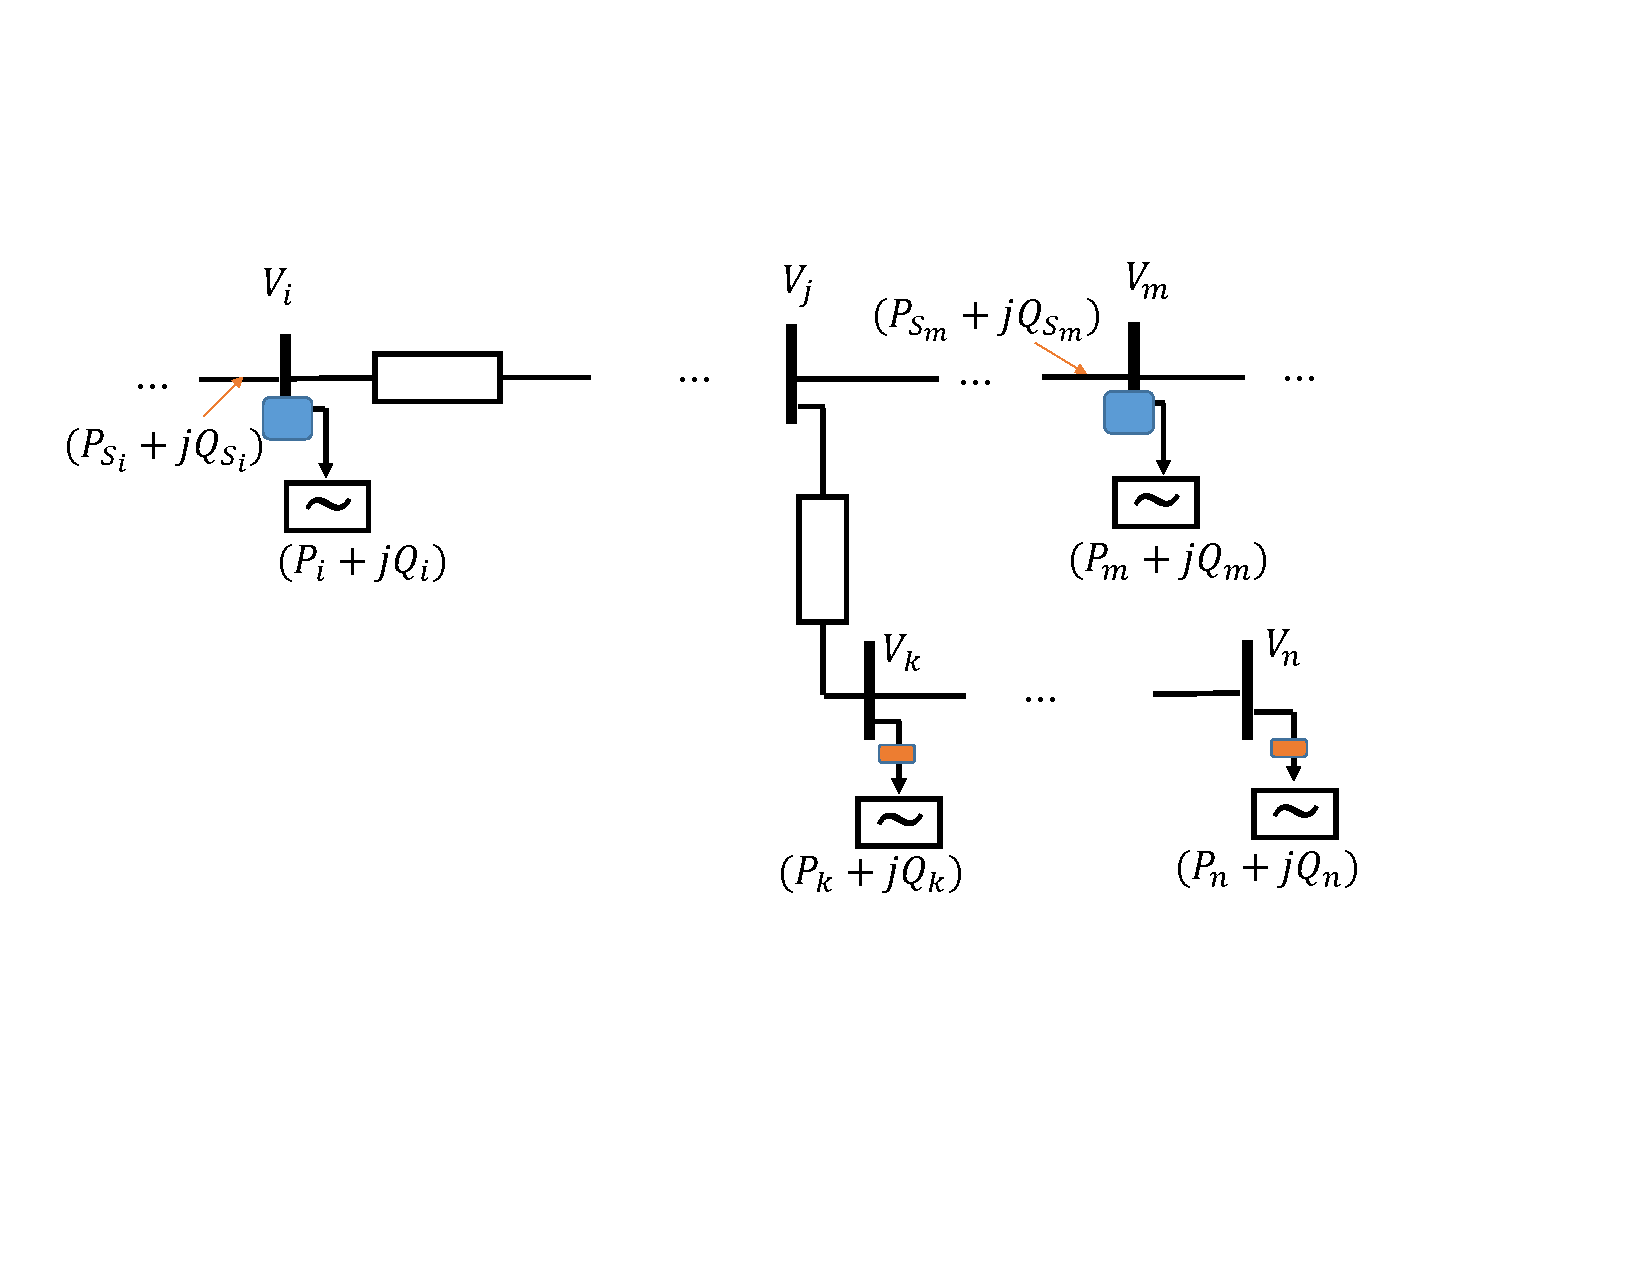
\includegraphics[width=\linewidth]{pics/vgrdnt3.pdf}
    \label{fig:mix}
    }
    \caption{Example of distribution network with measurements}
    \label{fig:vgrdnt}
\end{figure}

Let's assume bus $i$ as the relative root bus in both circuits: type (I) and (II), and also assume it is a SMU. So equation \eqref{eq:brchflowvpl} is applicable to all buses in both circuits considering bus $i$ as the slack bus: 
\begin{equation}
    V_k^2 =-\sum_{m\in\mathcal {P}_{ik}\cup \mathcal{T}_k} (2\mathcal{R}_{km}P_m+ 2\mathcal{X}_{km}Q_m+Z'_{km} P_{L_m})+V_i^2,\;\;k\in\mathcal{T}_i,\label{eq:vkr}
\end{equation}
where $V_i$ can be measured in real-time.

Define the sensitivities of voltage at bus $k$ to real and reactive power injection at bus $j$ by $ \zeta_{kj}$ and $ \xi_{kj}$ respectively:
\begin{equation}
    \zeta_{kj} \overset{\Delta}{=} \frac{\partial V_k}{\partial P_j} \text{ and } \xi_{kj} \overset{\Delta}{=} \frac{\partial V_k}{\partial Q_j}  ,
\end{equation}
then we can infer all AMU bus voltages by
\begin{equation}
V_k=    V_k^0 + \Delta V_k,
\end{equation}
where $V_k^0$ is the initial value and $\Delta V_k$ can be estimated by
\begin{equation}
    \Delta V_k  =-\sum_{ m \in\mathcal{P}_{ik}\cup \mathcal{T}_k} (\zeta_{km}\Delta P_m+ \xi_{km} \Delta Q_m).\label{eq:vklnr}
\end{equation}

Therefore, the key of voltage inference is the network sensitivity calculation, which will be discussed in the next subsection.
\subsection{Network sensitivity}
It follows \eqref{eq:vkr} that the sensitivities can be written as: 
\begin{equation}
    \zeta_{kj} \overset{\Delta}{=} -\frac{\mathcal{R}_{kj}}{V_k} -\frac{1}{2V_k}\sum_{m\in\mathcal {P}_{ik}\cup \mathcal{T}_k} Z'_{km} \frac{\partial P_{L_m}}{\partial P_j},
\end{equation}
and
\begin{equation}
    \xi_{kj} \overset{\Delta}{=} -\frac{\mathcal{X}_{kj}}{V_k} -\frac{1}{2V_k}\sum_{m\in\mathcal {P}_{ik}\cup \mathcal{T}_k} Z'_{km} \frac{\partial P_{L_m}}{\partial Q_j}.  
\end{equation} 
From the previous analysis, the system loss should always be relatively small compared to the power injection, e.g. the loss of the illustration example (Figure \ref{fig:3bussys}) are shown in Figure \ref{fig:dldpq}. As in the example, within the studied region of ($P_g$, $Q_g$), the derivatives are close to zero and monotonic along with the injection: loss is decreasing at the negative part, and increasing after certain point (zero).   
\begin{figure}[h!]
    \centering
    \subfloat[Loss to $P_g$]{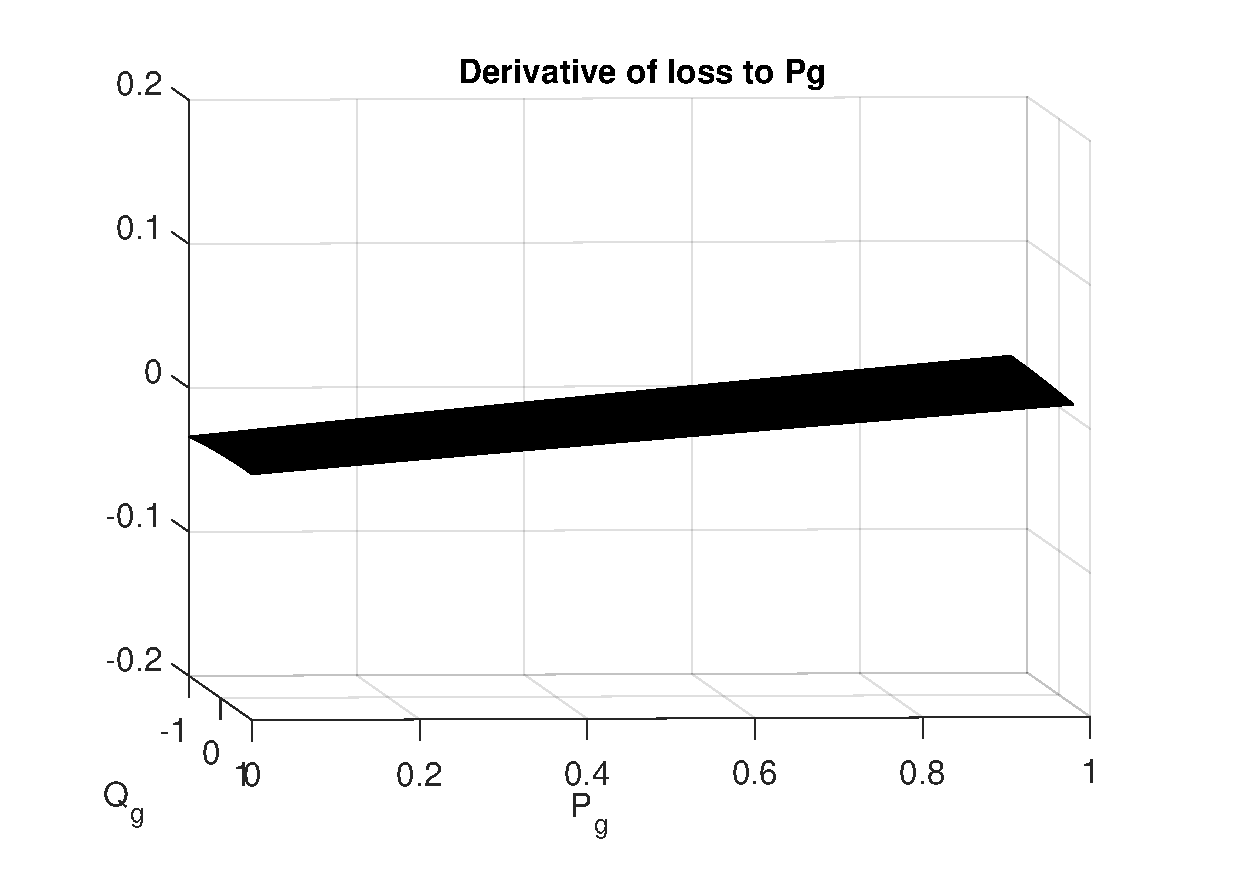
\includegraphics[width=\linewidth,height = 6cm]{pics/dldp.pdf}}
    \quad
    \subfloat[Loss to $Q_g$]{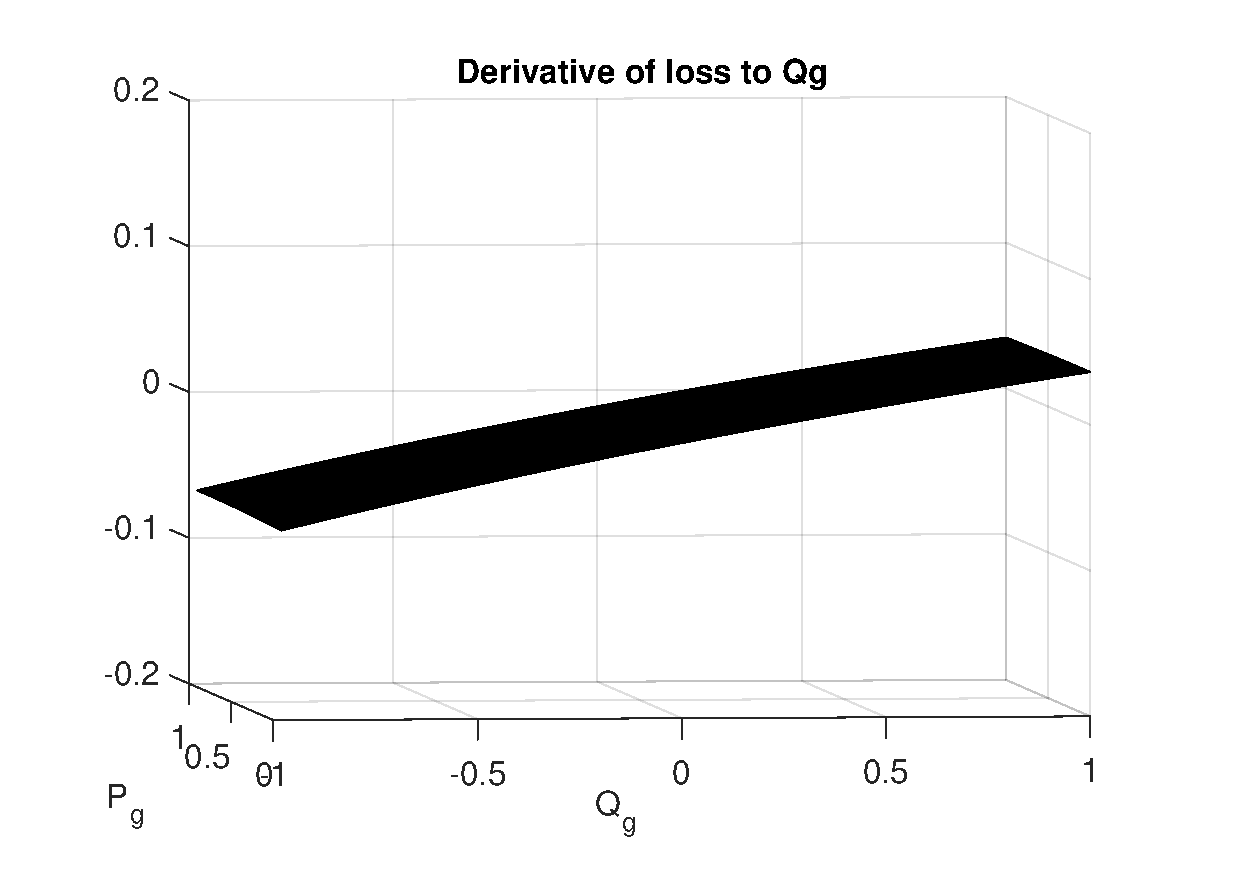
\includegraphics[width=\linewidth,height = 6cm]{pics/dldq.pdf}}
    \caption{The derivative of loss with respect to power injection}
    \label{fig:dldpq}
\end{figure}

By neglecting the system loss, the voltage sensitivities of real and reactive power can be written as follows:
\begin{equation}
    \zeta_{kj} \approx -\frac{\mathcal{R}_{kj}}{V_k} \text{ and } \xi_{kj}\approx -\frac{\mathcal{X}_{kj}}{V_k}. \label{eq:zxv}
\end{equation}
Using the illustration system, the above defined sensitivities of bus voltage with respect to real and reactive power injections are shown in Figure \ref{fig:dvdpq}. As the plots show, $V_i$ increases when the power $P_g$ and $Q_g$ increases, so that the derivatives slightly decrease. Also, it is clear that
\begin{equation}
 \zeta_{kj} \approx -\mathcal{R}_{kj} \text{ and } \xi_{kj}\approx -\mathcal{X}_{kj},   \label{eq:zetaxi}
\end{equation}
as shown in the illustration example ($\mathcal{R}_{kj}=0.025$ and $\mathcal{X}_{kj}=0.05$), and bus voltages are always close to $1\;p.u.$.
 \begin{figure}[ht]
    \centering
    \subfloat[Loss to $P_g$]{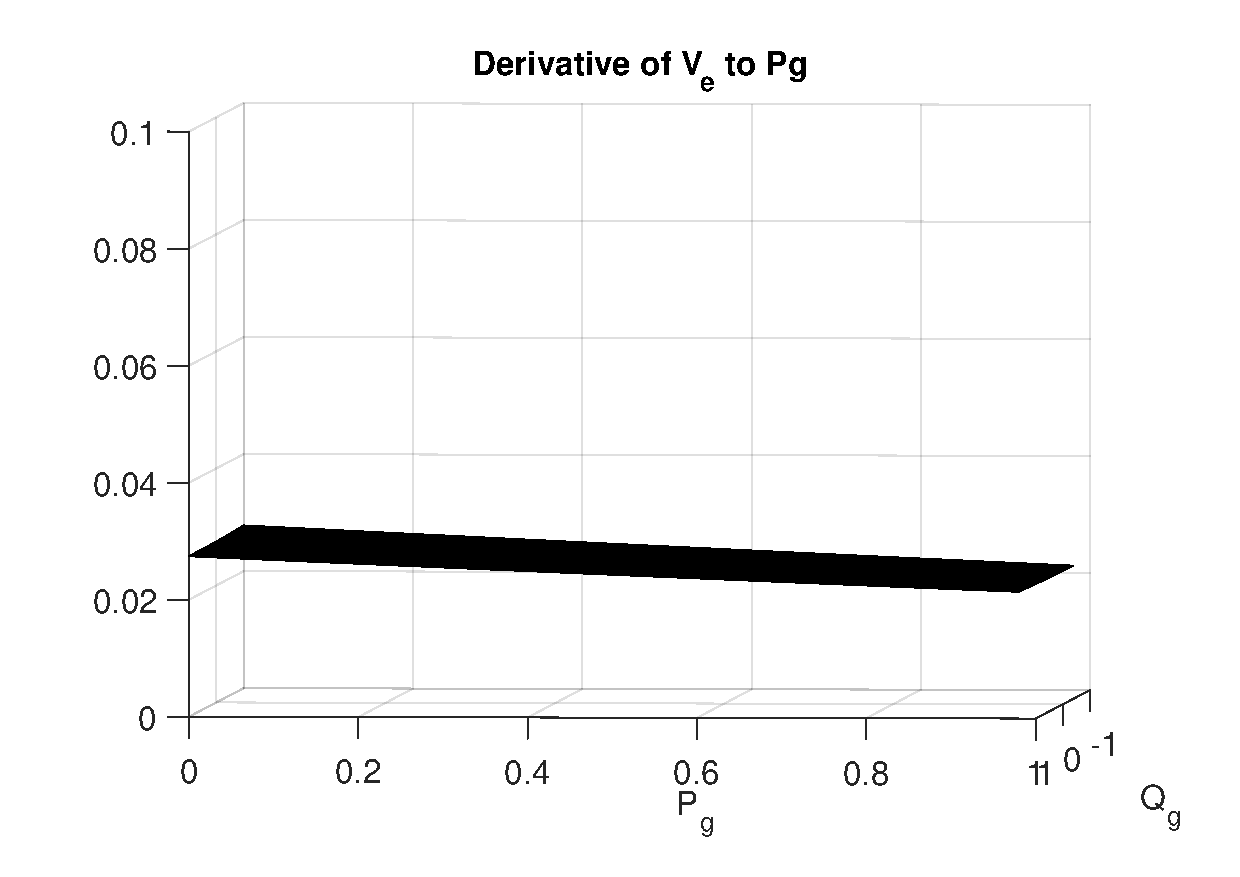
\includegraphics[width=\linewidth,height = 5cm]{pics/dvdp.pdf}}
    \quad
    \subfloat[Loss to $Q_g$]{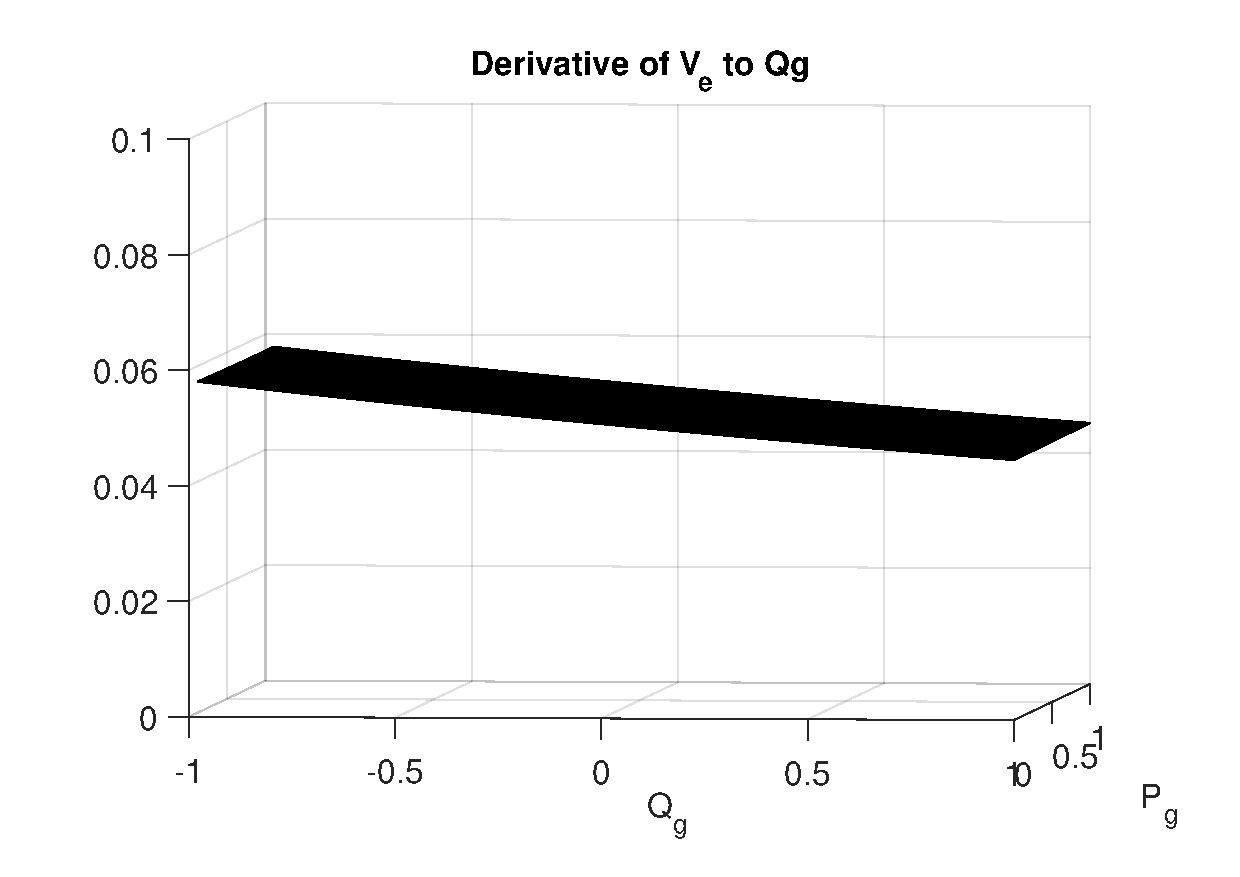
\includegraphics[width=\linewidth,height = 5cm]{pics/dvdq.pdf}}
    \caption{The derivative of loss with respect to power injection}
    \label{fig:dvdpq}
\end{figure}

Hence the voltage inference equation \eqref{eq:vklnr} is modified as the following application form:
\begin{equation}
   V_k=    V_k^0 -\sum_{ m \in\mathcal{P}_{ik}\cup \mathcal{T}_k} (\zeta_{km}\Delta P_m+ \xi_{km} \Delta Q_m),  \label{eq:vklvr-r}
\end{equation}
where $ V_k^0$ is the base value; $\Delta P_m$ and $\Delta Q_m$ represent the power fluctuation at AMU buses and will be discussed in the next subsection.

\subsection{Implementation}
From \eqref{eq:vklvr-r}, the last question for voltage inference is to determine the power injection of AMU buses. Use the proposed model \eqref{eq:vkliniear}, we use standard estimation methods to tackle this problem. Load estimation is not the focus of this paper, hence we will briefly describe the problem and will not expand the detailed process here.  
According to the setup, at time $T_t$, all the measurements from both SMUs and AMUs are known; in the time between $T_t$ and $T_{t+1}$, the information of SMUs is available while that of AMUs is not until $T_{i+1}$. Under the same assumption of neglecting system loss, the total power injection of all AMU buses (defined by $P_t+jQ_t$) can be calculated by applying Kirchhoff law in Figure \ref{fig:vgrdnt}: in type (I)
\begin{equation}
    P_t=P_{S_i}-P_i\text{ and }Q_t = Q_{S_i}-Q_i,
\end{equation}
and in type (II)
\begin{equation}
    P_t=P_{S_i}-P_i-P_{S_m}\text{ and }Q_t = Q_{S_i}-Q_i-Q_{S_m}.
\end{equation}

There are mainly four steps to implement the grid-edge situational awareness method: first, the total injection $P_t+jQ_t$ and voltage deviation $\Delta V_i$ (and/or $\Delta V_m$) can be obtained from measurement; second, using historical data and measurement at time $T_t$, we can apply one of the short-term prediction methods such as \cite{guan2013hyb,yu2012inte} to form a participation factor of each bus, then $P_t+jQ_t$ can be distributed among these buses; third, using the real time measurement at SMUs (voltage, power flow), standard estimation method, e.g. least square method, can be employed to improve the results of $\Delta P_m$ and $\Delta Q_m$; and last,
plugging them into \eqref{eq:vklvr-r} to solve $V_k$, which completes the inference process.

We use IEEE-123 system to test the performance of the proposed method. As shown in Figure \ref{fig:123-7}, 4 PVs are installed in the subtree of bus 72, two SMUs (blue stars) at bus  72 and 77, and 16 AMUs (red stars) at some other buses. Two stars are at bus 77, one for each case: case 1 with bus 77 as an AMU and case 2 with bus 77 as a SMU.
\begin{figure}[h!]
    \centering
    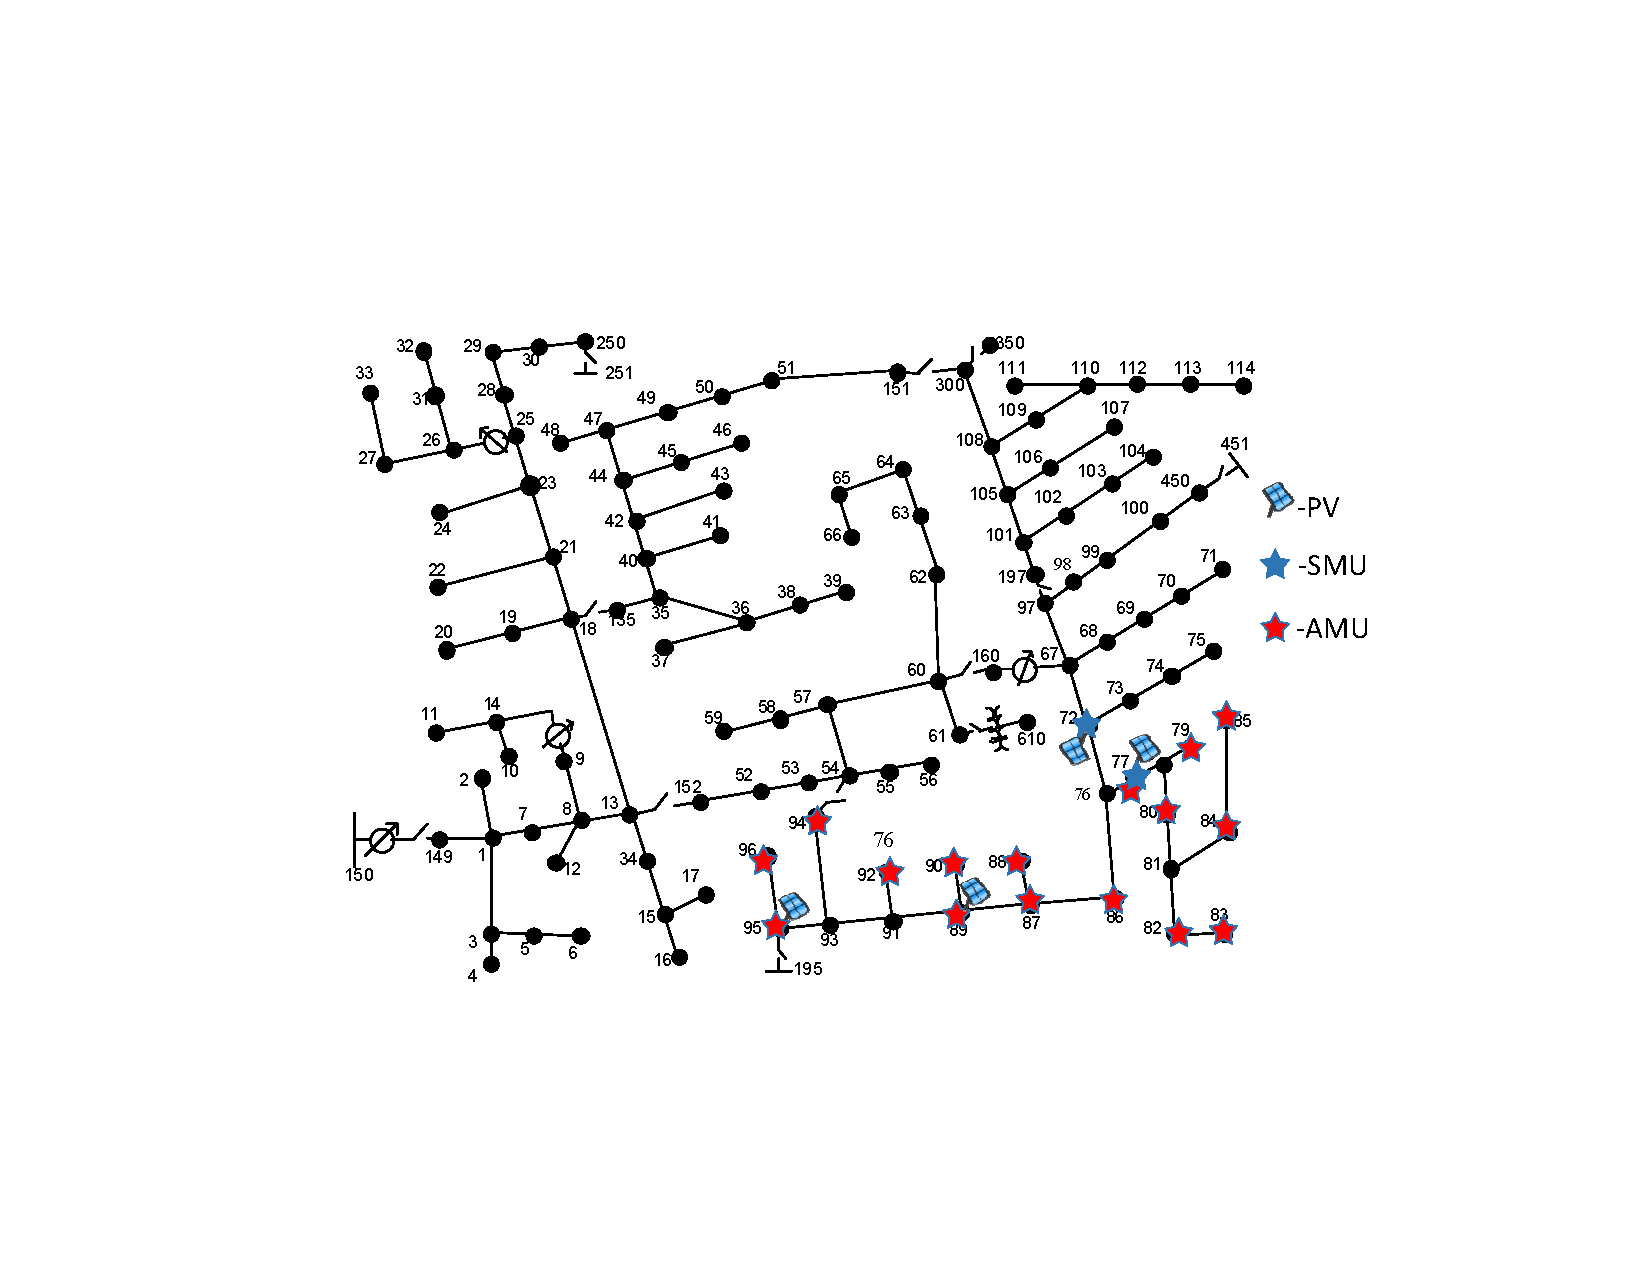
\includegraphics[width=\linewidth]{pics/123-7.pdf}
    \caption{IEEE 123 system with SMUs (blue stars), AMUs (red stars) } and PVs on bus 72, 77 and 89
    \label{fig:123-7}
\end{figure}

The sensitivities of bus voltages with respect to different real and reactvive power injections at bus 89 are shown in Figure \ref{fig:sens89}. The results are PU values with the base power as 3.6MVA and base voltage as 2.4kV. The lines are the results from simulation of changing the power injection at bus 89, while the stars are the approximated sensitivities at each bus using \eqref{eq:zetaxi} by the network parameters. It is clear that the the numerical results are close to the results approximated by system parameters. So in the case of fast calculation, network sensitivity can be roughly approximated by network parameters, i.e. $\zeta_{kj} \approx -\mathcal{R}_{kj} $ and $ \xi_{kj}\approx -\mathcal{X}_{kj}$. 
\begin{figure}[h!]
    \centering
    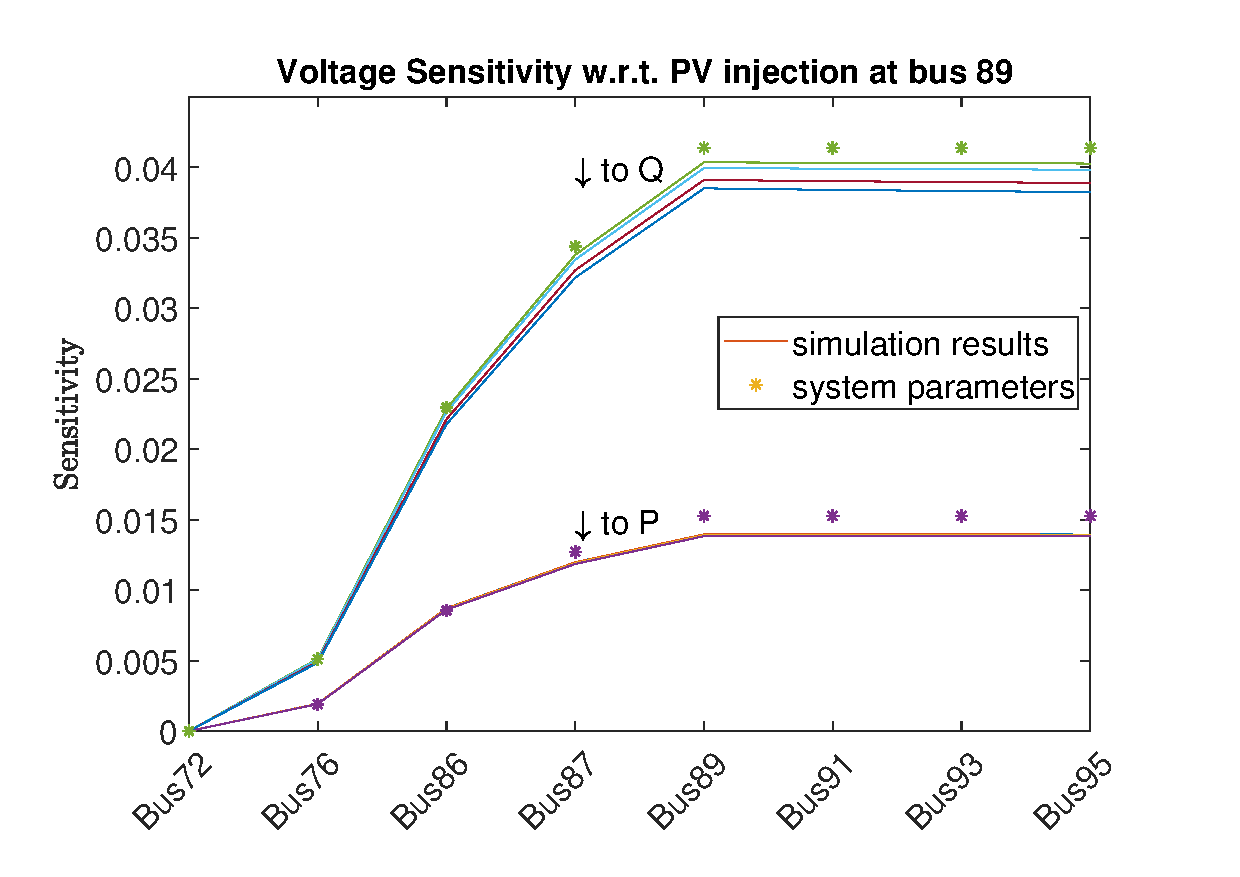
\includegraphics[width=\linewidth]{pics/sensitivity.pdf}
    \caption{Voltage sensitivity with respect to different real and reactive power injections}
    \label{fig:sens89}
\end{figure}

Case 1 is designed as type (I) voltage inference scenario, where no SMU is placed in the subtree of bus 72 (SMU). Assume that, at time $T_k$, all the measurements are available at bus 72, but all measurements from AMUs are not reachable at time $T_k+\Delta t$, $\Delta t \in (T_k ,T_{k+1})$. At time $T_k+\Delta t$, the voltage and the downstream (upstream) power at SMU can be measured; given a forecast load, the output of PVs can be estimated. Then bus voltages can be inferred by the proposed method. Simulation results in Figure \ref{fig:case1} show that the voltages can be accurately inferred. The red and blue lines are the system voltage lines of two scenarios with different PV allocations. The red one is worse because the load prediction is worse than the blue.  Case 2 is designed as type (II) voltage inference scenario, where another SMU is placed at bus 77. The extra information help improve the result, especially when the load change is larger in the subtree of bus 77. In this case, we set a load disturbance of PV 77. The results are shown in Figure \ref{fig:case2}, where the stars are results with real-time measurement at bus 77 and the diamons are without SMU there. It is obvious that the voltage inference results with real-time measurement are better than without real-time measurement. 

\begin{figure}[h!]
    \centering
\subfloat[case 1]{
    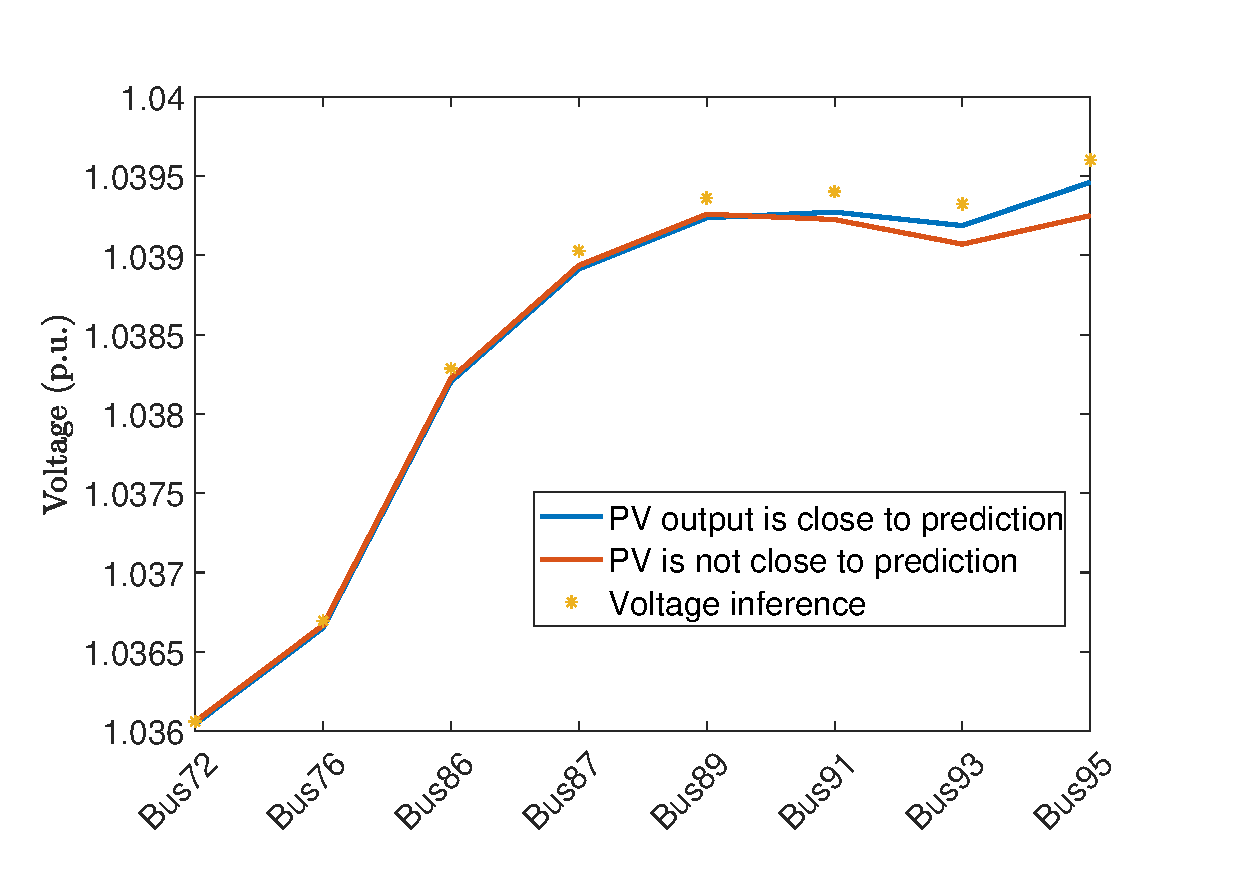
\includegraphics[width=0.85\linewidth]{pics/c7case1.pdf}
    \label{fig:case1}}
    \quad
\subfloat[case 2]{
    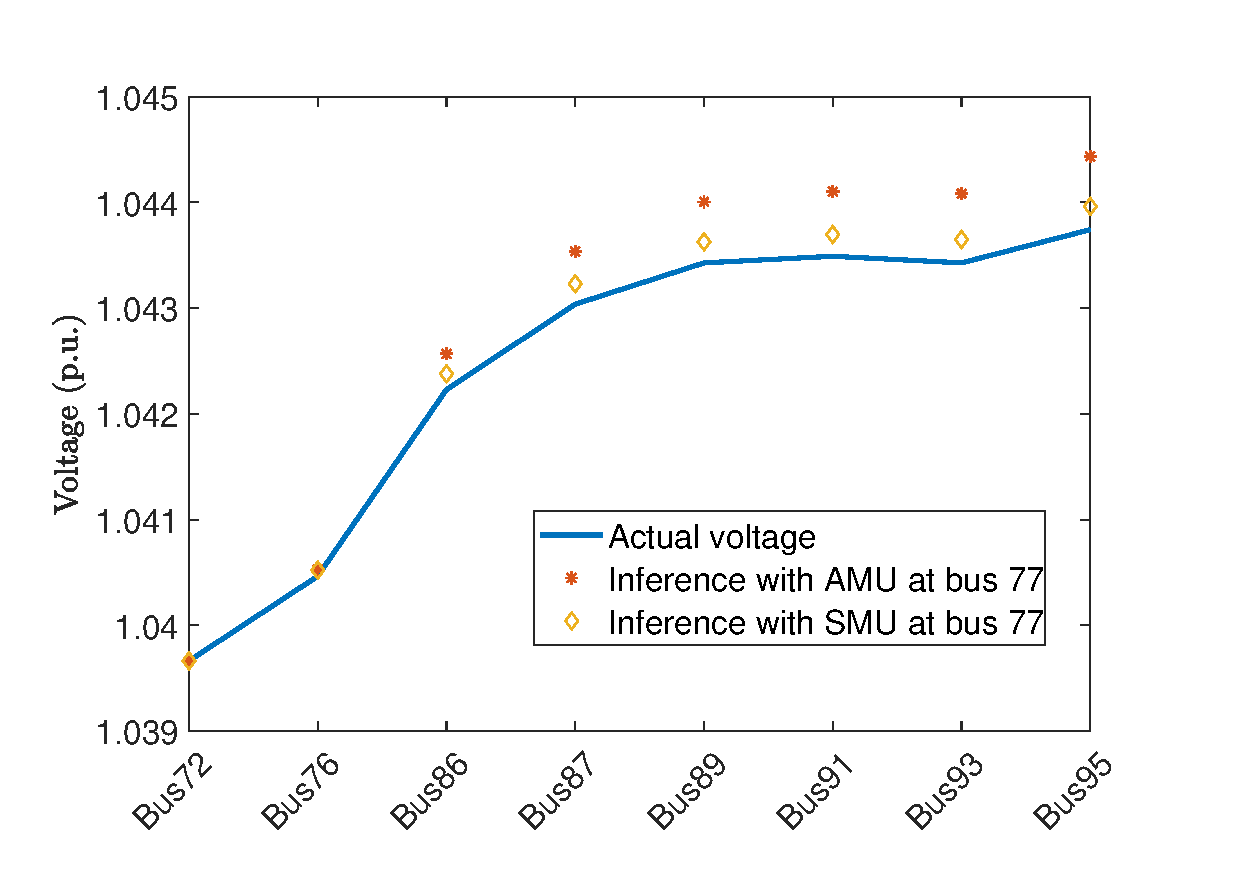
\includegraphics[width=0.85\linewidth]{pics/c7case2.pdf}
    \label{fig:case2}}
\caption{Simulation results of voltage inference on IEEE 123 system}
\end{figure}
 

\section{Control-enabled dynamic hosting allowance: P and Q control capacity and impact analysis}
\subsection{Traditional hosting analysis}
Hosting capacity (HC) is an important planning tool for both distribution system operators (DSOs) and DG investors to assess how much DG generation can be integrated into the distribution network \cite{ismael2019state}. It is a limit of the quantity of renewables allowed to be integrated without imposing any changes to the existing infrastructure and without
violating operational limits. Up until HC, DGs can be easily interconnected and could be approved through fast track process.

There are numerous unspecified factors for HC calculation, such as DER locations and capacities, control settings of feeder equipment such as voltage regulators, and the changing operational conditions (load level). The exhaustive detailed HC calculation is usually not preferred in practice, so instead the stochastic methods are widely used. Based on the trends observed from many detailed study cases, EPRI presented a streamline method to speed up HC calculation \cite{rylander2015streamlined}. However, all existing hosting analysis are generally conservative and require further development in the following aspects: 
\begin{enumerate}[label=$-$]
    \item To incorporate time-serious analysis using prediction and trend data other than worst-case snapshot data
    \item To involve advanced inverter control and complimentary DER technologies
    \item To explore rapid approaches for HC calculation and scanning
    \item To further study the inter-activities between DERs and the impact on HC
\end{enumerate}

It is very possible and feasible, along with the development of renewable technologies, to install more DER than HC either by upgrading or installing additional
equipment, or developing advanced operational and control strategies. 
Furthermore, HC is a system-oriented terminology and specific for planning. 
To the extent of system operation, it is required to go beyond the hosting capacity which needs more extensive and much faster
analysis and control strategy.
To this end, a network sensitivity -based dynamic hosting allowance (DHA) method is presented in this section, which includes both the operating condition and the control impact of DER inverters.

\subsection{Dynamic hosting allowance analysis}
Voltage problems specially voltage rise are considered as the most significant problem for high penetration of DG integration\cite{walla2012determining}, so the system-wide max voltage is a major factor in hosting analysis. 
As shown in Figure \ref{fig:trend}, the trend of maximum feeder-wide primary voltage in a particular deployment of PV with respect to penetration level appears roughly linear\cite{rylander2015streamlined}, but the physical nature behind this observation has not been discussed yet. 
\begin{figure}[h!]
    \centering
    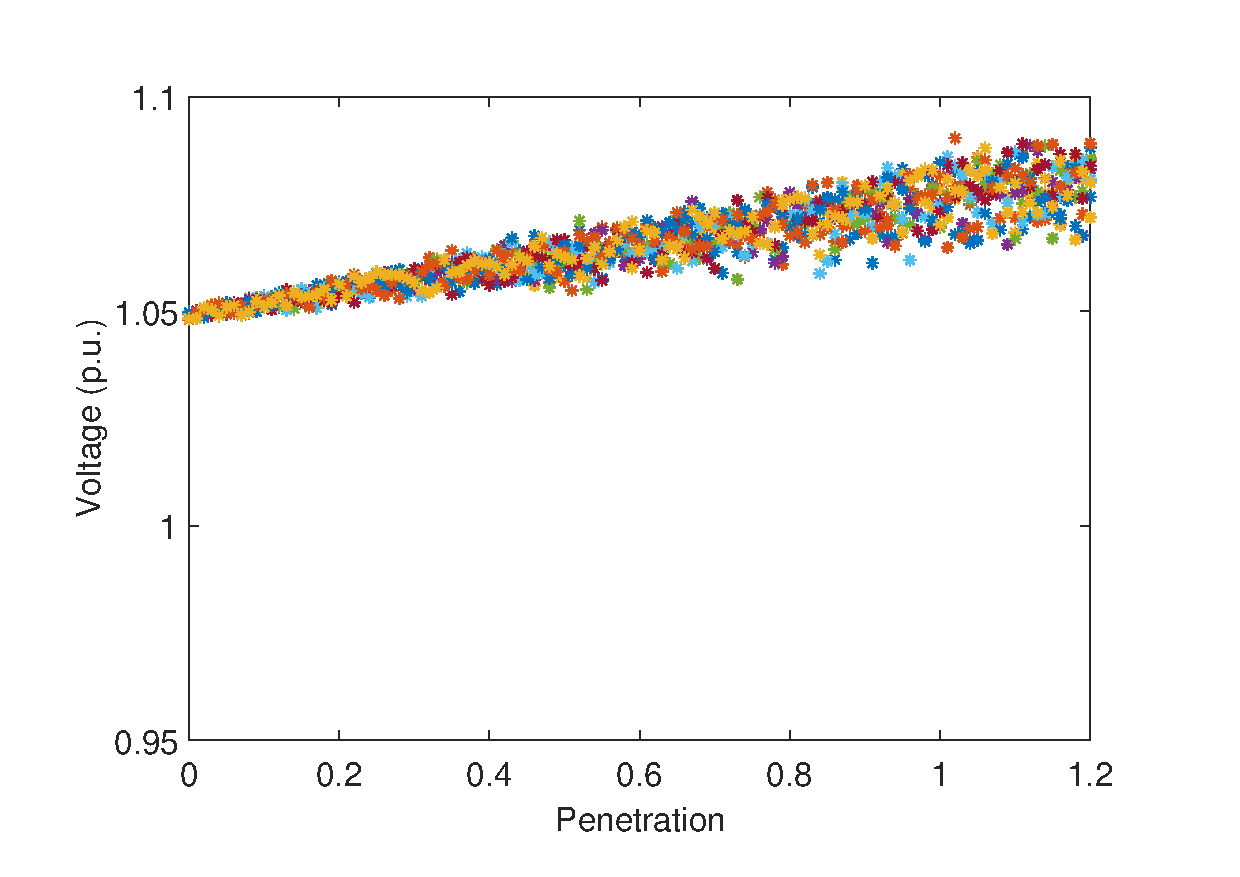
\includegraphics[width=0.9\linewidth]{pics/trend-3.pdf}
    \caption{System voltage shows a linear trend with respect to renewable penetration (IEEE 123 system)}
    \label{fig:trend}
\end{figure}
In the previous section, we built the network sensitivity, and through analysis, we found that the network sensitivity is a property of distribution network. Here we rewrite \eqref{eq:vklnr} by the following matrix form:
\begin{equation}
  \Delta V = \Pi \Delta P + \Xi \Delta Q, \label{eq:lZX}  
\end{equation}
where
\begin{equation}
  \Pi = \{\zeta_{kj}\}  \text{ and } \Xi = \{\xi_{kj}\}, \label{eq:ZX}  
\end{equation}
which can be approximated as constant (the system parameter of distribution network, $\mathcal{R}_{kj}$ and $\mathcal{X}_{kj}$). The properties of network sensitivity, i.e. $\Pi$ and $\Xi$, can explain the linear trend shown in Figure \ref{fig:trend}.

Using sensitivity matrix, we can improve the HC maps \cite{ismael2019state} by revealing the the additive effect of system-wide DERs to critical buses - dynamic hosting allowance (DHA). As shown in Figure \ref{fig:hcmap}, the traditional HC map did not answer the question of
how $P_i+jQ_i$ and $P_k+jQ_k$ contribute the critical voltage $V_n$; on the other hand, with certain head room of $V_n$ (and/or other critical bus voltages), how to strategically deploy $P_i+jQ_i$ and $P_k+jQ_k$, as well as the injection of other DERs. 
\begin{figure}[h!]
    \centering
    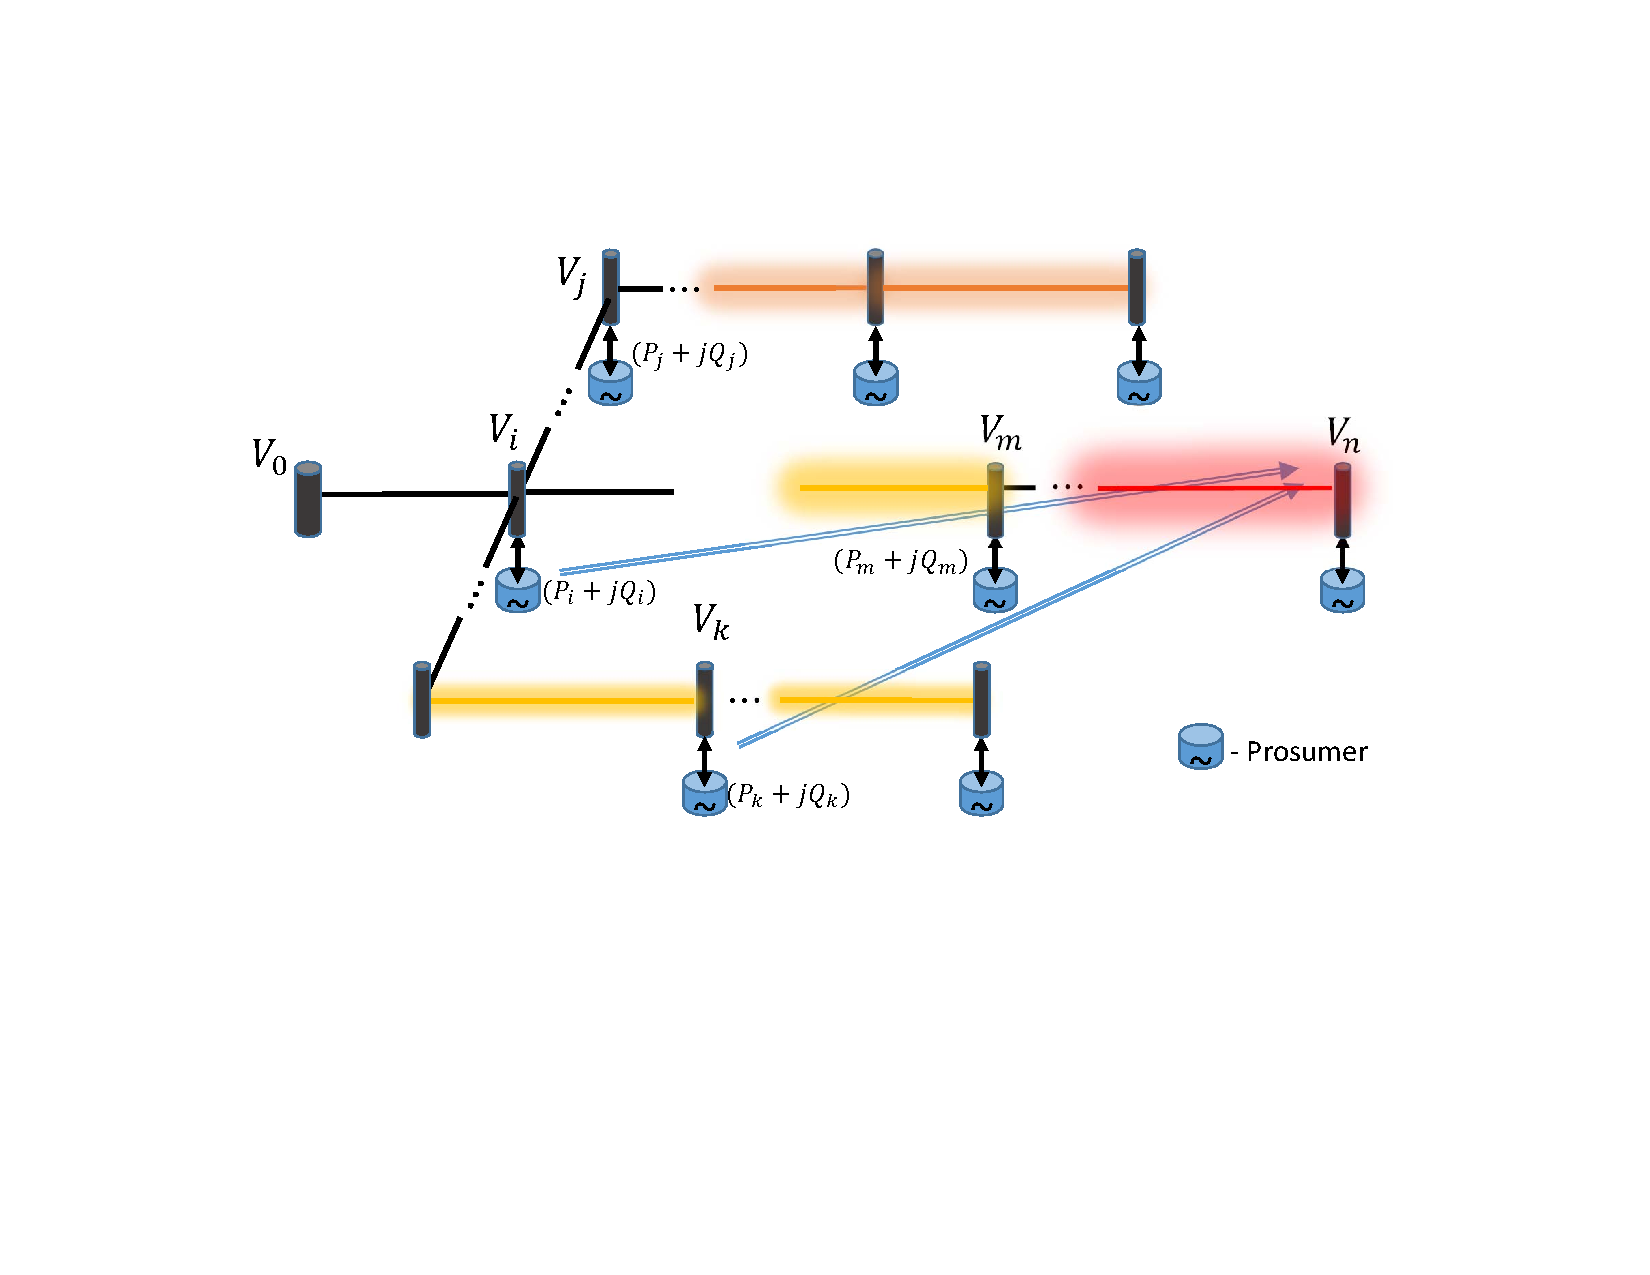
\includegraphics[width=0.75\linewidth]{pics/hcmap.pdf}
    \caption{HC map can indicate how HC varies along feeder segments using appropriate color coding in regards to the current percentage of each segment, but additive effect of different DGs to different bus voltages are not analyzed.}
    \label{fig:hcmap}
\end{figure}

As shown in Figure \ref{fig:dha}, the network sensitivity together with synchronous and asynchronous measurement can greatly improve the functionality of HC maps. This can be further extended into real-time DG operation and control (if the DG inverters are able to offer extra control ability). 
\begin{figure}[h!]
    \centering
    \subfloat[physical system]{
    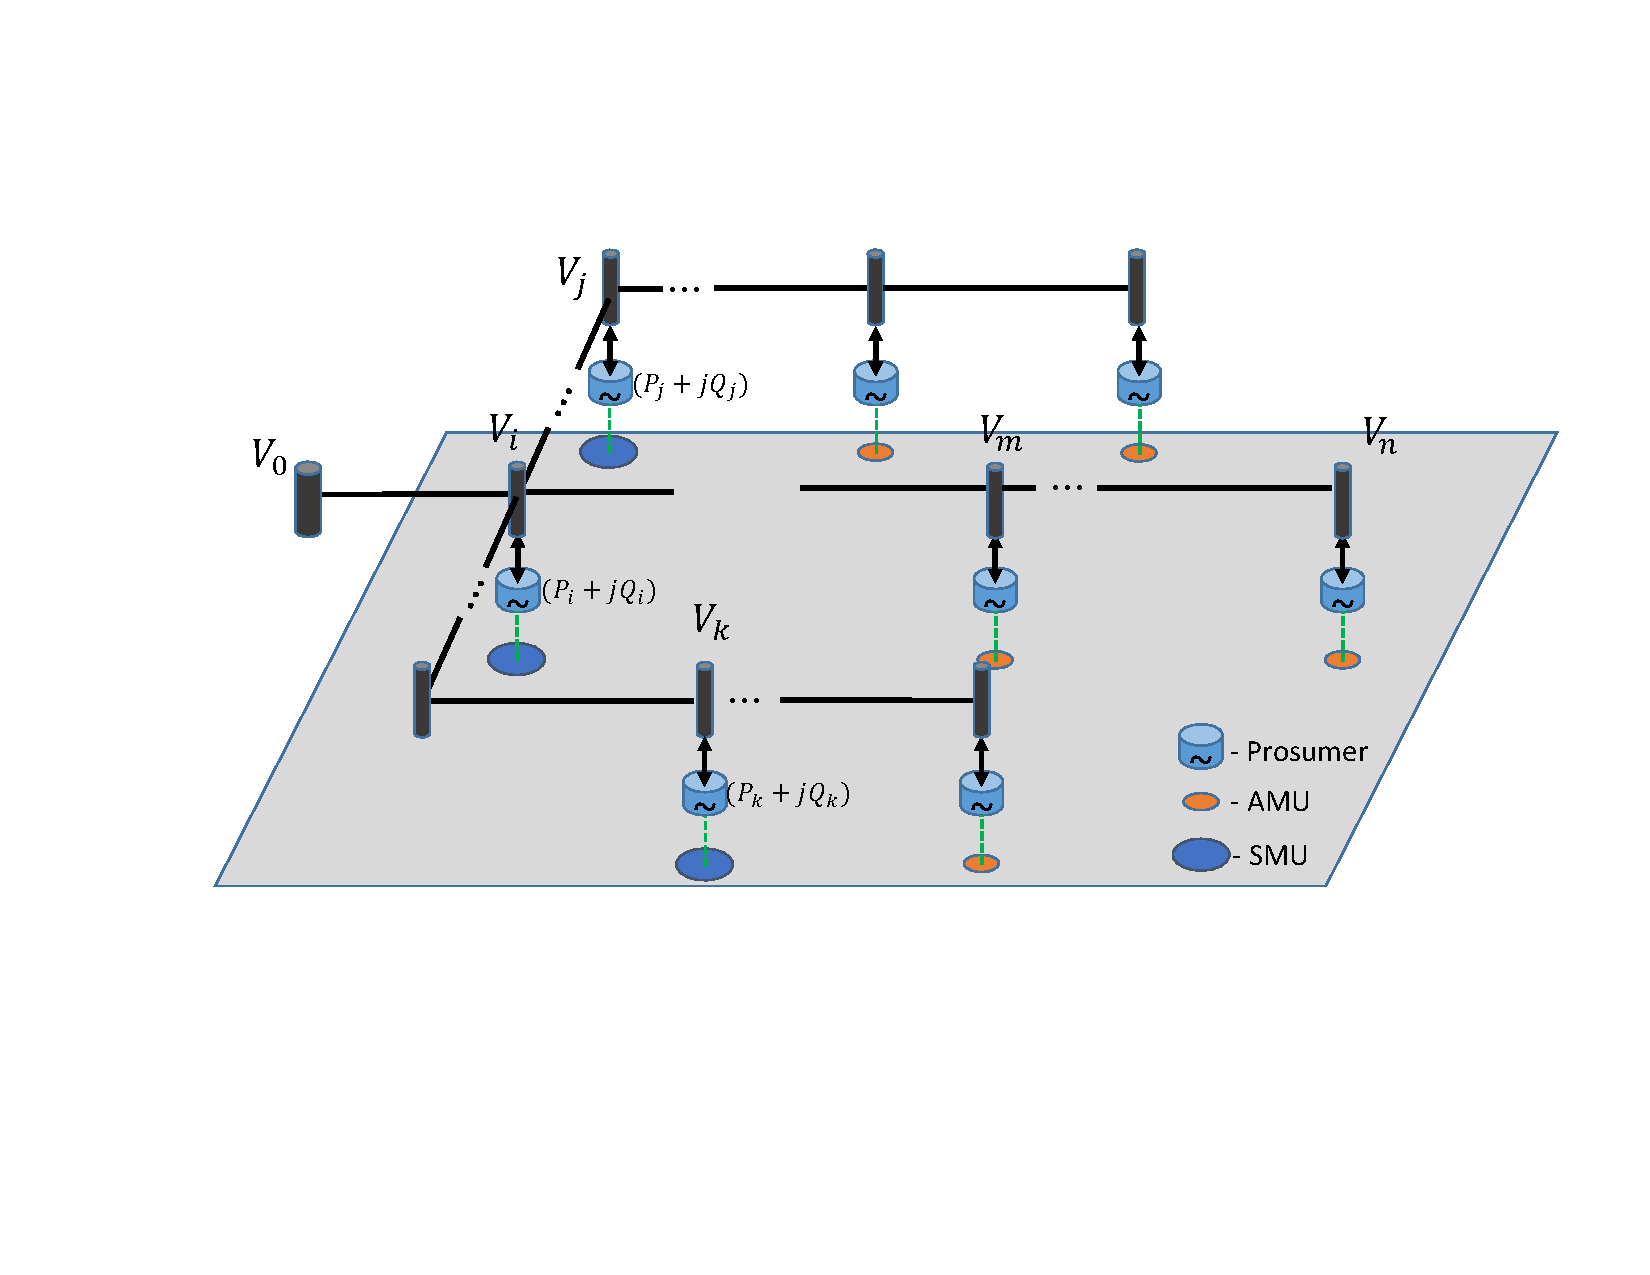
\includegraphics[width=0.75\linewidth]{pics/DHA.pdf}
    }
    \quad
    \subfloat[network sensitivity]{
    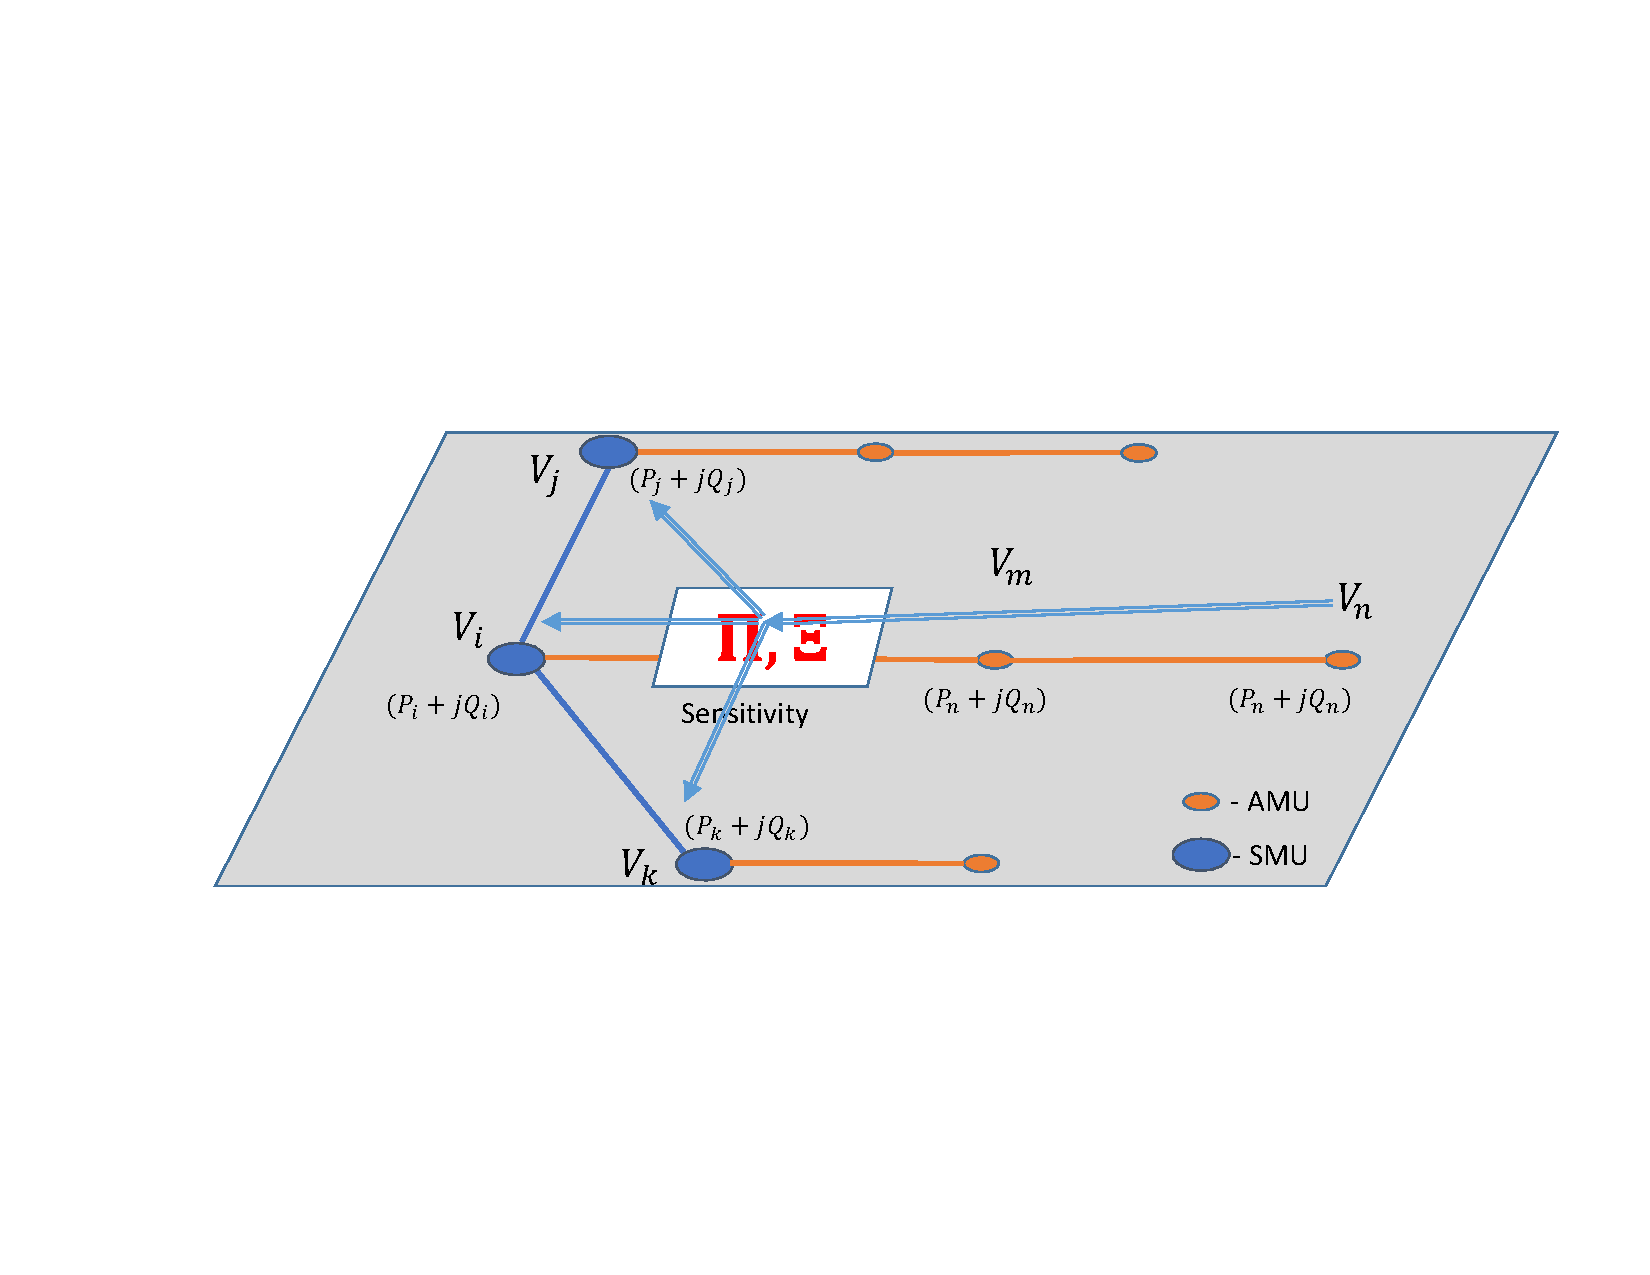
\includegraphics[width=0.75\linewidth]{pics/sens.pdf}
    }
    \caption{The sensitivity of system-wide DERs to the critical bus}
    \label{fig:dha}
\end{figure}

In the context of operation control, the critical bus voltage is the key factor of DHA. We can first identify the head room of critical voltage, which can be assessed through the grid-edge situational inference process. Assume the voltage head room of critical bus $n$ is $\Delta V_n$, then we have
\begin{equation}
    \Delta V_n = -\sum_{ m \in\mathcal{P}_{in}\cup \mathcal{T}_n} (\zeta_{nm}\Delta P_m+ \xi_{nm} \Delta Q_m).\label{eq:vnlnr}
\end{equation}
Then, with specific control strategy in the system, we can quickly calculate the DHA for system. For example, define a parameter as $\sigma$ to describe capability of inverter, that $S=(1+\sigma)\overline{P}$. we can calculate $\Delta Q_m$ by 
\begin{equation}
    \Delta Q_m = -\overline{Q}_m  = -\sqrt{\sigma^2+2\sigma} \overline{P}_m= -\sqrt{\sigma^2+2\sigma} (P_m+\Delta{P}_m), \label{eq:dltQ}
\end{equation}
and finally solve \eqref{eq:vnlnr} for $\Delta P$,
which is the result of DHA. Note that as reactive power control is enabled, the system current increase, hence the thermal limits should be checked. 

%\subsection{Simulation results}
We use IEEE 123-bus system to illustrate the DHA process. We use case 1 in previous section as the example to calculate DHA at bus 72 in IEEE 123-bus system. From the simulation results (Figure \ref{fig:sens89}) in the previous section, we know the network sensitivity has the property of monotonically increasing from root to the leaf side of the circuit. So the highest DHA of this part of the system should be DHA at bus 72 with the concern of voltage rise. From the results of case 1, we also know the voltage head room of this scenario is $\Delta V=1.05-1.0396=0.0104 pu$ (base power is 3.6 MW and base voltage is 2.4kV). Also we know that the real and reactive power sensitivities at bus 72 are $\zeta_{in} = 0.048701pu$ and $\xi_{in}=0.0936pu$. If reactive power control is not considered, the DHA at bus 72 can be directly calculated:
\begin{equation}
    \Delta P = \frac{\Delta V}{\zeta_{in}} = 0.2135pu.
\end{equation}
When reactive power control is enabled, we assume $\sigma=0.02$, then we can plug \eqref{eq:dltQ} into \eqref{eq:vnlnr} and solve $\Delta P$ as
\begin{equation}
    \Delta P = \frac{\Delta V+\sqrt{\sigma^2+2\sigma}\xi_{in}P}{\zeta_{in}-\sqrt{\sigma^2+2\sigma}\xi_{in}} = 0.52pu.
\end{equation}


\section{Co-simulation of integrated transmission and distribution systems}
\subsection{The framework of co-simulation}
\subsubsection{Integrated T\&D system simulation}
The co-simulation architecture of integrated T\&D system is developed as follows. The snapshot of transmission system power flow is first solved, and the voltage at each bus connected with the distribution systems are saved. Each distribution system is assigned a process with parameters of voltage levels, circuit name and process number. Once each process is established, they start and execute simultaneously. The various sizes and complexity of distribution systems cause the power flow to solve in different time duration. Thus, the algorithm waits for the convergence of all distribution systems before sending the real and reactive power values at the substation back to the transmission bus. A text file is generated containing the real and reactive power at the substation after each power flow solution with respect to the transmission voltage. The transmission system power flow is then solved again with the updated parameters. The algorithm iterates through this process until the $\Delta V \leq 0.0001$. In summary, the co-simulation architecture follows the following steps:\par

\begin{enumerate}[label=S-$\arabic*$.]
    \item Load and solve transmission system
    \item Assign a distribution system to 10 of the load buses
    \item Extract $V_{pu}$ at each load bus
    \item Define a process for each distribution system with its corresponding voltage value
    \item Solve each distribution system in parallel
    \item Send P and Q from substation node to the transmission system
    \item Update transmission load bus with P and Q obtained from distribution
    \item Repeat steps 1-7 until $\Delta V_{pu}$ (of each load bus) $\leq 0.001$\par
\end{enumerate}

The integrated T\&D system co-simulation architecture was modeled and simulated using co-simulation of Python and MA-OpenDSS. Loads in the buses of transmission system were analyzed to determine real and reactive power values which resembled the total real and reactive power of various distribution systems. Once the buses were identified, the distribution systems are allocated to each individually. Python was used to interface with MA-OpenDSS and facilitate the usage of parallel processing when solving the power flow of each of the distribution systems. \par

\subsubsection{Parallel co-simulation of integrated T\&D systems}
The parallel simulation was performed on the distribution systems while the transmission system waited to receive the real and reactive power values. The same type of simulation was performed but in a sequential manner. The distribution systems ran one at a time while the transmission system waited for the results. This was done to compare and verify the results. When running the distribution systems in sequence, the simulation time was increased, but real and reactive power values remained the same. Simulation results show that even though the sequential simulation of each distribution system tends to be slightly faster than parallel simulation (less processing power required to run one distribution system at a time), it takes longer to complete the overall simulation. While the parallel simulation is bottlenecked by the simulation of largest distribution system, the sequential simulation waits for one distribution circuit to converge before running the next, thus taking much longer time to perform the integrated T\&D simulation.\par

The simulation framework has been implemented on the latest version of MA-OPenDSS with the parallel capability, which allows different distribution networks to be simulated in parallel by assigning them to different cores in a multi-core computer. This makes it scalable to handle multiple large-scale distribution networks in integrated T/D studies.\par

\subsection{Simulation Results}
\subsubsection{Power flow of integrated T\&D systems}
The topology of T\&D co-simulation is shown in Fig. \ref{fig:tdsimulation}. The T\&D test system consists of an IEEE 14-bus transmission system with three detailed distribution networks: IEEE 8,500-node system, 11,000-node (IEEE8,500 + EPRI Circuit 7) system, and 100,000-node (12 of 8,500-node circuits) system. The system can easily be expanded by replacing lumped transmission-level loads with distribution networks.\par

\begin{figure}[h]
    \centering
    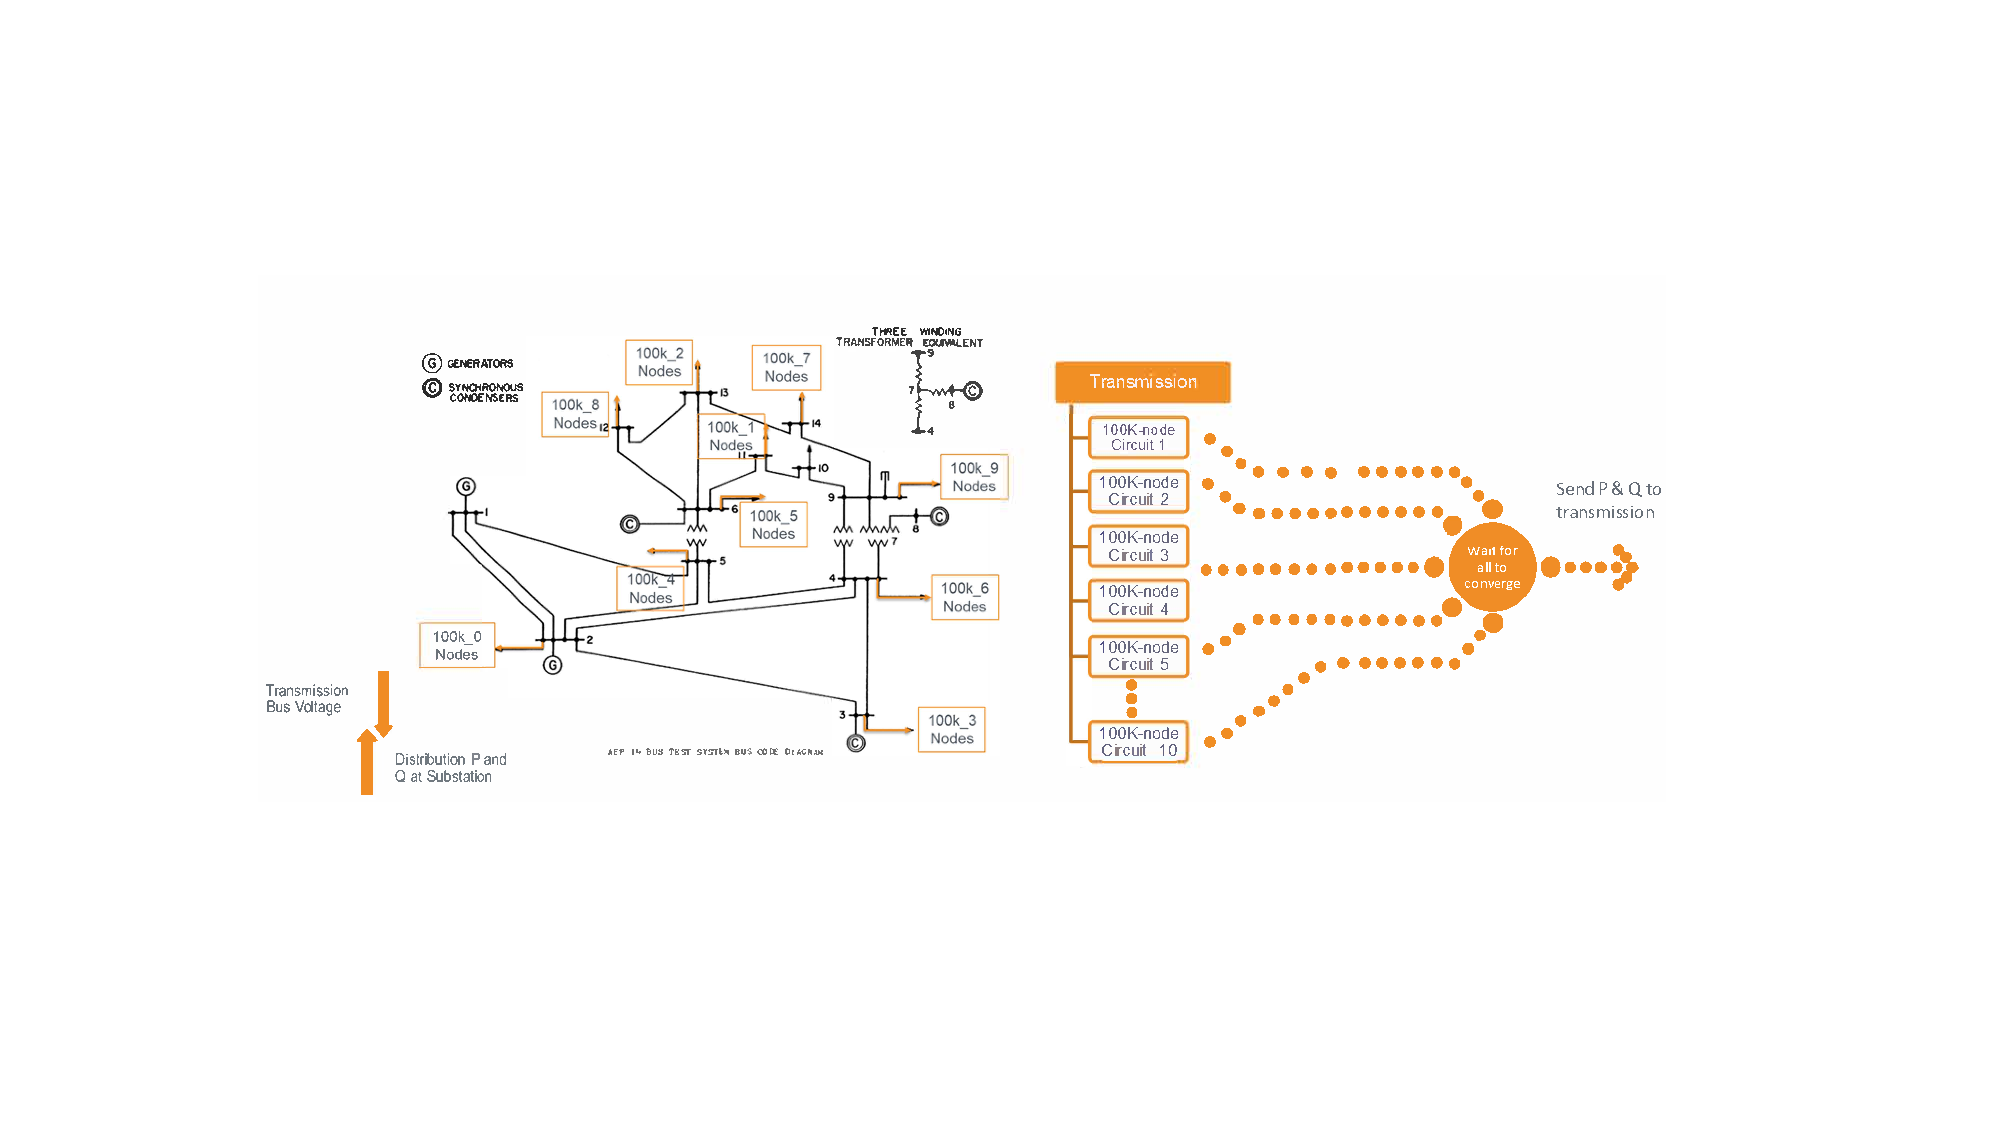
\includegraphics[width=1.0\linewidth]{pics/tdsimulation.pdf}
    \caption{Integrated T\&D simulation topology}
    \label{fig:tdsimulation}
\end{figure}

Table \ref{tab:tdsimulation1} shows the simulation results of 4 iterations with total 27 seconds of simulation time. One can observe the response of distribution systems to various voltage changes in each iteration. \par

\begin{table}[h]
\centering
\caption{Simulation results of integrated T\&D study}
\resizebox{\textwidth}{!}{
\begin{tabular}{|l|l|l|l|l|l|l|l|l|l|}
\hline
   & \multicolumn{3}{c|}{8.5k Nodes}  & \multicolumn{3}{c|}{11k Nodes}   & \multicolumn{3}{c|}{100k Nodes}     \\
\hline
Ite & V Bus 13 & P         & Q        & V Bus 11 & P         & Q         & V Bus 14 & P          & Q          \\
\hline
1   & 0.9495   & 10092.358 & 2707.363 & 0.9495   & 77552.727 & 35871.226 & 0.9493   & 144610.512 & 21991.715  \\
\hline
2   & 0.9666   & 10422.447 & 2760.587 & 0.9665   & 79997.143 & 36923.693 & 0.9664   & 144026.118 & 18664.282  \\
\hline
3   & 0.9660   & 10410.870 & 2758.983 & 0.9659   & 79907.645 & 36887.208 & 0.9658   & 144055.285 & 18825.498  \\
\hline
4   & 0.9659   & 10409.064 & 2758.731 & 0.9658   & 79894.028 & 36881.875 & 0.9657   & 144059.901 & 18850.989 \\
\hline
\end{tabular}}
\label{tab:tdsimulation1}
\end{table}

The 14-bus transmission system can be scaled up to accommodate for ten 100K-node distribution circuits located at each of its load buses. Preliminary simulation of ten 100K-node distribution circuits was executed in both parallel and sequential manners without any transmission connection, in order to compare the computation time. For sequential simulation, each of the ten circuits took approximately 4.7 seconds to solve, and the overall simulation time was about 53 seconds (exporting results, setting up the systems counts are part of the total simulation time). On the other hand, the parallel simulation of ten circuits resulted in a total of 35 seconds, which counts for one iteration of the integrated T\&D without the transmission power flow simulation time. Thus, it can be projected that there will be a tremendous benefit in reducing computation time. Furthermore, a faster machine with more processing power and core availability can improve the parallel processing computation time.\par

\subsubsection{Integrated T\&D systems with PVs and control}
PVs and control are added to the integrated T\&D systems. A synthetic 100,000-node NREL System with 100$\%$ penetration of small-scale PVs and distributed control was selected as the distribution system. Table \ref{tab:tdsimulation2} displays the real and reactive power for the base case, the case adding PVs without control, and the case adding PVs with control.\par

\begin{table}[h]
\caption{T\&D co-simulation cases}
\centering
\begin{tabular}{|l|l|l|}
\hline
Simulation Type      & P (kW)    & Q (kW)   \\ \hline
1) Base Case         & 123,992.6 & 48,282.3 \\ \hline
2) PVs, No Control   & -870.58   & 38,468.4 \\ \hline
3) PVs, With Control & -1,052.5  & 66,138.5 \\ \hline
\end{tabular}
\label{tab:tdsimulation2}
\end{table}\par

When PVs are present, the reactive power demand increases significantly (approximately 1.4 times the base case) in order to address over-voltage problems. On the other hand, the distribution system is supplying the transmission with about 1.05MW. In order to address high reactive power demand, capacitor banks are placed on the secondary side (12.47kV) of 14 feeders of NREL-100k system. Two T\&D co-simulations were carried out with an aggregated capacitance of 110.8Mvar and 153.5Mvar, as shown in Table \ref{tab:tdsimulation3}. Two capacitor banks were used in order to address the fluctuations of the substation voltage.\par

\begin{table}[h]
\caption{T\&D co-simulation cases with capacitor banks}
\centering
\resizebox{\textwidth}{!}{
\begin{tabular}{|l|l|l|l|}
\hline
Simulation Type     & Aggregated Capacitance (Mvar) & P (kW)    & Q (kvar)  \\ \hline
4) DG, With Control & 110.80 (12.47kV)              & -1,147.8  & -390.2    \\ \hline
5) DG, With Control & 153.50 (12.47kV)              & -1,192.26 & -34,922.2 \\ \hline
\end{tabular}}
\label{tab:tdsimulation3}
\end{table}\par

Table \ref{tab:tdsimulation4} displays T\&D co-simulation results of three different simulation scenarios: 3), 4), and 5). The distribution system was connected to bus 11 of the IEEE 14-bus system, considering the smaller load at this bus (3.5MW, 1.8Mvar). It can be observed that it takes 9 iterations to converge without the capacitor banks. On the order hand, it takes 5 and 4 iterations to converge with aggregated capacitor banks of 110.8Mvar and 153.50Mvar, respectively.\par

Another observation can be made with respect to the difference in total reactive power supplied by the capacitors. Although the power factor at the substation when solving distribution system power flow is much better with the total Q of 110.80Mvar provided by capacitor banks, this is not the case when the voltage changes at the transmission side. The reactive power shifts from supplying 390.2kvar to transmission to demanding 8,370.72kvar from transmission. Meanwhile, the feeder supplies reactive power when there is approximately 43Mvar increase in the total capacitor banks. Further studies can be performed in order to find the optimal capacitor placement and capacity in order to maintain a relatively reasonable power factor. \par

\begin{table}[h]
\caption{Comparison of T\&D co-simulation cases with capacitor banks}
\centering
\resizebox{\textwidth}{!}{
\begin{tabular}{|l|l|l|l|l|l|l|l|l|}
\hline
\multicolumn{3}{|l|}{3) No Qbank} & \multicolumn{3}{l|}{4) Qbank = 110.80Mvar} & \multicolumn{3}{l|}{5) Qbank=153.50Mvar} \\ \hline
V(pu)     & P(kW)    & Q(kvar)    & Voltage      & P(kW)         & Q(kvar)     & V(pu)        & P(kW)      & Q(kvar)      \\ \hline
1.0179    & -1038    & 62519      & 1.04536      & -1070.58      & 8527.31     & 1.0179       & -1022      & -35725       \\ \hline
0.9341    & -2824    & 21250      & 1.04418      & -1101.21      & 8354.14     & 1.06945      & -1009      & -30867       \\ \hline
1.0154    & -1167    & 60371      & 1.04439      & -1084.81      & 8364.2      & 1.06955      & -1070      & -30698       \\ \hline
0.9398    & -2847    & 26773      & 1.04446      & -1079.17      & 8366.38     & 1.06956      & -1069      & -30699       \\ \hline
1.0068    & -1566    & 51582      & 1.04453      & -1074.32      & 8370.72     &              &            &              \\ \hline
0.9602    & -2458    & 45637      &              &               &             &              &            &              \\ \hline
0.9736    & -2344    & 47560      &              &               &             &              &            &              \\ \hline
0.9697    & -2396    & 47585      &              &               &             &              &            &              \\ \hline
0.9698    & -2363    & 47592      &              &               &             &              &            &              \\ \hline
\end{tabular}}
\label{tab:tdsimulation4}
\end{table}

\newpage
\section{Conclusion}
This chapter presented a hierarchical distributed control framework to model, analyze, optimize and control large-scale distribution system with extremely high penetration of renewables. Following the layered and divisional principle for large-scale power system planning, the Voltage/VAR control is mainly treated as a local control ; while the real power control is a system-level control (frequency) and a supplementary control for local voltage, which will respond only when reactive power control is insufficient. 
For electrical circuit, both nodal injection and branch power flow models are used to model distribution network; and a simplified power control model of DG is used, which is simple but good enough to illustrate the design of system operation and control. A detailed analysis of the system-level effect of local autonomous controls is presented in this chapter. Also, how the presented control runs in islanded mode of the distribution system is provided.
To tackle the problem of low observability in distribution network, a sensitivity-based grid-edge situational awareness method is presented for distribution system state estimation, control and optimization. Following that, a network sensitivity -based dynamic hosting allowance (DHA) method is presented for system operation, as an extensive and much faster analysis compared to the traditional hosting capacity. At last, to validate the feasibility and demonstrate the scalability of developed models and algorithms, a co-simulation architecture of integrated T\&D system is developed.


\bibliographystyle{unsrtnat}
\bibliography{references}
\end{document}